% Options for packages loaded elsewhere
\PassOptionsToPackage{unicode}{hyperref}
\PassOptionsToPackage{hyphens}{url}
%
\documentclass[
]{book}
\usepackage{lmodern}
\usepackage{amssymb,amsmath}
\usepackage{ifxetex,ifluatex}
\ifnum 0\ifxetex 1\fi\ifluatex 1\fi=0 % if pdftex
  \usepackage[T1]{fontenc}
  \usepackage[utf8]{inputenc}
  \usepackage{textcomp} % provide euro and other symbols
\else % if luatex or xetex
  \usepackage{unicode-math}
  \defaultfontfeatures{Scale=MatchLowercase}
  \defaultfontfeatures[\rmfamily]{Ligatures=TeX,Scale=1}
\fi
% Use upquote if available, for straight quotes in verbatim environments
\IfFileExists{upquote.sty}{\usepackage{upquote}}{}
\IfFileExists{microtype.sty}{% use microtype if available
  \usepackage[]{microtype}
  \UseMicrotypeSet[protrusion]{basicmath} % disable protrusion for tt fonts
}{}
\makeatletter
\@ifundefined{KOMAClassName}{% if non-KOMA class
  \IfFileExists{parskip.sty}{%
    \usepackage{parskip}
  }{% else
    \setlength{\parindent}{0pt}
    \setlength{\parskip}{6pt plus 2pt minus 1pt}}
}{% if KOMA class
  \KOMAoptions{parskip=half}}
\makeatother
\usepackage{xcolor}
\IfFileExists{xurl.sty}{\usepackage{xurl}}{} % add URL line breaks if available
\IfFileExists{bookmark.sty}{\usepackage{bookmark}}{\usepackage{hyperref}}
\hypersetup{
  pdftitle={O czym śpiewają Holendrzy?},
  pdfauthor={Jacek Pardyak},
  hidelinks,
  pdfcreator={LaTeX via pandoc}}
\urlstyle{same} % disable monospaced font for URLs
\usepackage{longtable,booktabs}
% Correct order of tables after \paragraph or \subparagraph
\usepackage{etoolbox}
\makeatletter
\patchcmd\longtable{\par}{\if@noskipsec\mbox{}\fi\par}{}{}
\makeatother
% Allow footnotes in longtable head/foot
\IfFileExists{footnotehyper.sty}{\usepackage{footnotehyper}}{\usepackage{footnote}}
\makesavenoteenv{longtable}
\usepackage{graphicx}
\makeatletter
\def\maxwidth{\ifdim\Gin@nat@width>\linewidth\linewidth\else\Gin@nat@width\fi}
\def\maxheight{\ifdim\Gin@nat@height>\textheight\textheight\else\Gin@nat@height\fi}
\makeatother
% Scale images if necessary, so that they will not overflow the page
% margins by default, and it is still possible to overwrite the defaults
% using explicit options in \includegraphics[width, height, ...]{}
\setkeys{Gin}{width=\maxwidth,height=\maxheight,keepaspectratio}
% Set default figure placement to htbp
\makeatletter
\def\fps@figure{htbp}
\makeatother
\setlength{\emergencystretch}{3em} % prevent overfull lines
\providecommand{\tightlist}{%
  \setlength{\itemsep}{0pt}\setlength{\parskip}{0pt}}
\setcounter{secnumdepth}{5}
% new for polish
\usepackage{polski}
\usepackage[polish]{babel}
%\usepackage[utf8]{inputenc}

% ------------
\usepackage{booktabs}
\usepackage{amsthm}
\makeatletter
\def\thm@space@setup{%
  \thm@preskip=8pt plus 2pt minus 4pt
  \thm@postskip=\thm@preskip
}
% ------------
% new for columns
\newenvironment{columns}[1][]{}{}

\newenvironment{column}[1]{\begin{minipage}{#1}\ignorespaces}{%
\end{minipage}
\ifhmode\unskip\fi
\aftergroup\useignorespacesandallpars}

\def\useignorespacesandallpars#1\ignorespaces\fi{%
#1\fi\ignorespacesandallpars}

\makeatletter
\def\ignorespacesandallpars{%
  \@ifnextchar\par
    {\expandafter\ignorespacesandallpars\@gobble}%
    {}%
}
\makeatother
\usepackage[]{natbib}
\bibliographystyle{apalike}

\title{O czym śpiewają Holendrzy?}
\author{Jacek Pardyak}
\date{2020-05-20}

\begin{document}
\maketitle

{
\setcounter{tocdepth}{1}
\tableofcontents
}
\hypertarget{wstux119p}{%
\chapter*{Wstęp}\label{wstux119p}}
\addcontentsline{toc}{chapter}{Wstęp}

\begin{column}{0.10\textwidth}

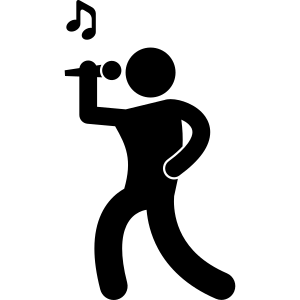
\includegraphics{./images/Wstep}

\end{column}

\begin{column}{0.04\textwidth}

~

\end{column}

\begin{column}{0.86\textwidth}

O czym śpiewają Holendrzy? O życiu i o umieraniu, o miłości i o rozstaniu, o kraju i o dupie. Książkę napisałem w języku R\footnote{GNU R -- interpretowany język programowania oraz środowisko do obliczeń statystycznych i wizualizacji wyników.}, źródła są dostępne w repozytorium GITHUB\footnote{\url{https://github.com/JacekPardyak/Liedboek}}. Nie mogę wskazać źródeł niderlandzkich tekstów, gdyż te wszędzie zawierają jakieś błędy. Jednakże wszelkie prawa do tekstów piosenek umieszczonych w tej książce przysługują ich właścicielom i nie mam zamiaru tego zmieniać. Teksty piosenek po wielu przeróbkach znajdują się tutaj wyłącznie w celach informacyjnych i edukacyjnych oraz służą do użytku prywatnego. Autorem tłumaczeń jestem ja. Tłumacząc starałem się utrzymać funkcjonalność oryginalnego tekstu. Jeżeli w przekazie są emocje, to chciałem je również czuć w tłumaczeniu. Chciałem przy tym zachować oryginalne słownictwo, a idiomy zastępować ich polskimi odpowiednikami. W żadnym przypadku nie było moją intencją dokonywać adaptacji piosenek ani tworzyć własnych odpowiadających melodii. Każda piosenka wzbogacona jest zbiorem wyrażeń żywego języka używających słów, wyrażeń bądź konstrukcji gramatycznych z piosenki. Są tam również wyjaśnienia nazw własnych, wszystko po to, by móc zrozumieć tekst jeszcze lepiej. Wszystkie grafiki stworzyłem sam bądź użyłem udostępnionych na licencji CCBY. Książka jest dostępna w formatach HTML, PDF i EPUB na stronie książki\footnote{\url{https://jacekpardyak.github.io/Liedboek/}}. Z radością przyjmę wszelką konstruktywna krytykę za pośrednictwem forum książki\footnote{\url{http://pub31.bravenet.com/forum/2597320020/}}.

\end{column}

\vfill

\hypertarget{Do-tanca}{%
\chapter{Do tańca}\label{Do-tanca}}

\begin{column}{0.10\textwidth}

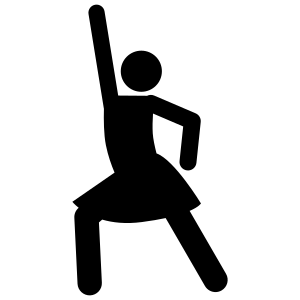
\includegraphics{./images/Do-tanca}

\end{column}

\begin{column}{0.04\textwidth}

~

\end{column}

\begin{column}{0.86\textwidth}

To są pisoenki do tańca

\end{column}

\vfill

\hypertarget{Hij-is-van-mij}{%
\section{\texorpdfstring{Hij is van mij, \emph{Kris Kross Amsterdam \& Maan \& Tabitha ft. Bizzey }}{Hij is van mij, Kris Kross Amsterdam \& Maan \& Tabitha ft. Bizzey }}\label{Hij-is-van-mij}}

\begin{column}{0.10\textwidth}

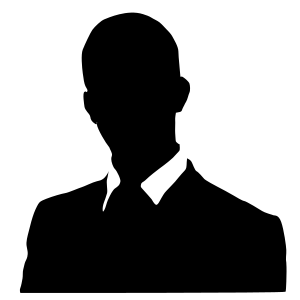
\includegraphics{./images/Hij-is-van-mij}

\end{column}

\begin{column}{0.04\textwidth}

~

\end{column}

\begin{column}{0.86\textwidth}

\textbf{Hij is van mij} \citep{Hij-is-van-mij} \href{https://youtu.be/EYhLEHE1vfQ}{\includegraphics{./images/youtube/_Youtube}} \emph{On jest mój} to luźny cover `The Boy Is Mine' amerykańskiego duetu Brenda i Monica. W 2019 roku był najlepiej sprzedającym się singlem w Holandii.

\end{column}

\vfill

\begin{column}{0.48\textwidth}

Voor het eerst in m'n leven\\
Kan ik iemand alles geven\\
Ik voel me veiliger bij je\\
Ja, hij heeft alles wat ik zoek\\
Ik hou `m extra dicht bij me\\
Want al die meiden die kijken\\
Maar hij geeft me geen twijfel

\end{column}

\begin{column}{0.04\textwidth}

~

\end{column}

\begin{column}{0.48\textwidth}

Po raz pierwszy w moim życiu\\
Mogę komuś oddać wszystko\\
Przy tobie czuję się bezpieczniej\\
Tak, on ma wszystko, czego szukam\\
Trzymam go bardzo blisko przy sobie\\
Przez te wszystkie dziewczyny, które się patrzą\\
Ale on nie pozwala mi wątpić

\end{column}

\vfill

\begin{column}{0.48\textwidth}

\emph{- Wat ik met hem wil begrijp jij niet}\\
\emph{- Verspil je tijd niet langer, alsjeblieft}\\
\emph{- Jij bent in de war, hij hoort bij mij}\\
\emph{- Dat is niet wat hij zei tegen mij}

\end{column}

\begin{column}{0.04\textwidth}

~

\end{column}

\begin{column}{0.48\textwidth}

\emph{- Nie rozumiesz, czego chcę z nim}\\
\emph{- Nie marnuj więcej czasu, proszę cię}\\
\emph{- Gubisz się, on należy do mnie}\\
\emph{- To nie jest to, co on mi powiedział}

\end{column}

\vfill

\begin{column}{0.48\textwidth}

\emph{Hij is van mij}\\
\emph{Hij zegt dat ik alles voor hem ben}\\
\emph{Dat ik hem het allerbeste ken}\\
\emph{Dat hij aan mij denkt op elk moment}\\
\emph{Hij is van mij}\\
\emph{Het maakt niet uit wat je van mij dacht}\\
\emph{Meisje, weet je niet dat `ie op mij wacht?}\\
\emph{Ik doe hem het beste elke nacht}\\
\emph{Hij is van mij}

\end{column}

\begin{column}{0.04\textwidth}

~

\end{column}

\begin{column}{0.48\textwidth}

\emph{On jest mój}\\
\emph{On mówi, że jestem dla niego wszystkim}\\
\emph{Że znam go najlepiej}\\
\emph{Że myśli o mnie w każdej chwili}\\
\emph{On jest mój}\\
\emph{To nie ma znaczenia, co o mnie myślisz}\\
\emph{Dziewczyno, czy nie wiesz że on na mnie czeka?}\\
\emph{Robię mu to najlepiej każdej nocy}\\
\emph{On jest mój}

\end{column}

\vfill

\begin{column}{0.48\textwidth}

Hij is het voor mij, geen andere heeft het\\
Hoe hij mij voelt kan niemand beter\\
Hij neemt me voorbij, beter weten\\
Hij heeft m'n naakt, ik zeg het elke dag\\
Ik zeg het elke dag

\end{column}

\begin{column}{0.04\textwidth}

~

\end{column}

\begin{column}{0.48\textwidth}

On jest dla mnie tym kimś, żadna inna tego nie ma\\
Jak on mnie wyczuwa nie potrafi nikt więcej\\
On bierze mnie do końca, lepiej wiedzieć\\
On ma moje nagie, mówię że codziennie\\
Mówię że codziennie

\end{column}

\vfill

\begin{column}{0.48\textwidth}

Ey, je zeurt aan m'n hoofd, mama\\
Kijk me in m'n ogen aan\\
Als je mij niet gelooft, mama (Ey, ey, ey)\\
Wat betekent dit dan allemaal?\\
Ik vind het moeilijk om te zeggen hoe het voelt\\
Dat er niks anders is wat ik mis, nee

\end{column}

\begin{column}{0.04\textwidth}

~

\end{column}

\begin{column}{0.48\textwidth}

Hej, marudzisz mi nad głową, mała\\
Spójrz mi w oczy\\
Skoro mi nie wierzysz, mała (Hej, hej, hej)\\
Co zatem znaczy to wszystko?\\
Trudno mi powiedzieć, jak to jest\\
Że nie brakuje mi niczego więcej, nie

\end{column}

\vfill

\begin{column}{0.48\textwidth}

Jou beschermen, dat is mijn doel\\
Courtois op die bitch, ik mis niks\\
Ik hou van make-up seks, maar dit gaat te ver, uh\\
We don't need to go there (Ooh)\\
You don't wanna go there

\end{column}

\begin{column}{0.04\textwidth}

~

\end{column}

\begin{column}{0.48\textwidth}

Bronić ją, to jest mój cel\\
Courtois na tę sukę, nic nie przepuszczę\\
Kocham uprawiać seks, ale to idzie za daleko, uch\\
Nie musimy tam iść (Ooch)\\
Nie chcesz tam iść

\end{column}

\vfill

\begin{column}{0.48\textwidth}

\emph{- Maan, hij is van mij, niet van jou maar van mij, oh}\\
\emph{- Tabitha hij is van mij, alleen van mij}

\end{column}

\begin{column}{0.04\textwidth}

~

\end{column}

\begin{column}{0.48\textwidth}

\emph{- Maan, on jest mój, nie twój, ale mój, och}\\
\emph{- Tabitha, on jest mój, tylko mój}

\end{column}

\vfill

\begin{column}{0.10\textwidth}

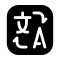
\includegraphics{./images/youtube/_Notes}

\end{column}

\begin{column}{0.001\textwidth}

~

\end{column}

\begin{column}{0.899\textwidth}

\begin{itemize}
\tightlist
\item
  \textbf{Je zou beter moeten weten.} Powinieneś wiedzieć lepiej.\\
\item
  \textbf{Neem vrij tot dit voorbij is.} Weź wolne dopóki to się nie skończy.\\
\item
  \textbf{Kan ik je wat water geven?} Czy mogę ci podać trochę wody?\\
\item
  \textbf{Ik voel me gevleid.} Schlebiasz mi.\\
\item
  \textbf{Ik voel me moe.} Czuję się zmęczony.\\
\item
  \textbf{Ik wil met je meegaan.} Chcę iść z tobą.\\
\item
  \textbf{Ik ben in de war.} Gubię się.\\
\item
  \textbf{Thibaut Nicolas Marc Courtois is een Belgische voetballer die dienstdoet als doelman.} Thibaut Nicolas Marc Courtois to belgijski piłkarz grający w drużynie jako bramkarz.
\end{itemize}

\end{column}

\vfill

\hypertarget{Links-en-rechts}{%
\section{\texorpdfstring{Links en rechts, \emph{Nick \& Simon}}{Links en rechts, Nick \& Simon}}\label{Links-en-rechts}}

\begin{column}{0.10\textwidth}

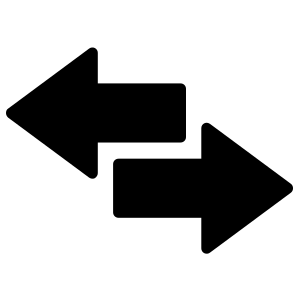
\includegraphics{./images/Links-en-rechts}

\end{column}

\begin{column}{0.04\textwidth}

~

\end{column}

\begin{column}{0.86\textwidth}

\textbf{Links en rechts} \citep{Links-en-rechts} \href{https://youtu.be/miac8oRrEcI}{\includegraphics{./images/youtube/_Youtube}} \emph{W lewo i w prawo} NOTE.

\end{column}

\vfill

\begin{column}{0.48\textwidth}

\emph{Ik wil naar links, jij gaat naar rechts}\\
\emph{Dus loop ik jou weer achterna}\\
\emph{Ik wil vooruit, jij achteruit}\\
\emph{Maar we komen toch weer bij elkaar}

\end{column}

\begin{column}{0.04\textwidth}

~

\end{column}

\begin{column}{0.48\textwidth}

\emph{Ja chcę w lewo, ty idziesz w prawo}\\
\emph{Dlatego znów chodzę za tobą}\\
\emph{Ja chcę do przodu, ty z powrotem}\\
\emph{Mimo to znów tak się spotykamy}

\end{column}

\vfill

\begin{column}{0.48\textwidth}

Met jou weet ik nooit waar ik aan toe ben\\
Met jou weet ik nooit precies wat jij bedoelt\\
Maar wat ik zeker weet en wat ik niet meer vergeet\\
Dat is dat jij hetzelfde voor mij voelt

\end{column}

\begin{column}{0.04\textwidth}

~

\end{column}

\begin{column}{0.48\textwidth}

Z tobą nigdy nie wiem, na czym stoję\\
Z tobą nigdy nie wiem dokładnie, co masz na myśli\\
Ale to, co wiem na pewno i czego nigdy nie zapomnę\\
Jest to, że ty wobec mnie czujesz to samo

\end{column}

\vfill

\begin{column}{0.48\textwidth}

Ik wordt een beetje moe van al dat wachten\\
Ik wordt een beetje moe van, we zien wel hoe het gaat\\
Wanneer hebben wij een keer alles uitgepraat\\
Dat jouw neus dezelfde kant op staat

\end{column}

\begin{column}{0.04\textwidth}

~

\end{column}

\begin{column}{0.48\textwidth}

Zaczynam być trochę zmęczony całym tym czekaniem\\
Zaczynam być tym trochę zmęczony, zobaczymy co z tego wyjdzie\\
Kiedy wszystko wyjaśnimy raz na dobre\\
Twoja głowa obróci się w tą samą stronę

\end{column}

\vfill

\begin{column}{0.48\textwidth}

Ik zeg ja en jij zegt nee\\
Jij gaat altijd je eigen weg\\
Maar op die weg is plaats voor twee\\
Onthoudt dus goed wat ik je zeg

\end{column}

\begin{column}{0.04\textwidth}

~

\end{column}

\begin{column}{0.48\textwidth}

Ja mówię tak, ty mówisz nie\\
Zawsze idziesz własną drogą\\
Ale na tej drodze jest miejsce dla dwojga\\
Zapamiętaj dobrze, co do ciebie mówię

\end{column}

\vfill

\begin{column}{0.10\textwidth}

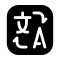
\includegraphics{./images/youtube/_Notes}

\end{column}

\begin{column}{0.001\textwidth}

~

\end{column}

\begin{column}{0.899\textwidth}

\begin{itemize}
\tightlist
\item
  \textbf{Ze zullen je als 'n hond achterna zitten.} Będą cię ścigać jak psa.\\
\item
  \textbf{We kennen elkaar niet.} My się nie znamy.\\
\item
  \textbf{Weet je, we zien wel.} Wiesz co, zobaczymy.\\
\item
  \textbf{Ik wil nog één keer alles nakijken.} Chcę wszystko jeszcze raz sprawdzić.\\
\item
  \textbf{Welke kant is het strand op?} W którą stronę jest plaża?\\
\item
  \textbf{Oké, goed dat we dit uitgepraat hebben.} Okej, dobrze że mamy to wyjaśnione.\\
\item
  \textbf{Met een bijdrage van 3 euro per neus kan iedereen overigens de actie steunen.} Każdy może wesprzeć akcję wkładem w wysokości 3 euro na głowę.\\
\item
  \textbf{Wanneer wij alles hebben gedaan, dan gaan wij een biertje drinken.} Kiedy wszystko zrobimy, napijemy się piwa.
\end{itemize}

\end{column}

\vfill

\hypertarget{Suzanne}{%
\section{\texorpdfstring{Suzanne, \emph{VOF de Kunst}}{Suzanne, VOF de Kunst}}\label{Suzanne}}

\begin{column}{0.10\textwidth}

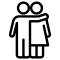
\includegraphics{./images/Suzanne}

\end{column}

\begin{column}{0.04\textwidth}

~

\end{column}

\begin{column}{0.86\textwidth}

\textbf{Suzanne} \citep{Suzanne} \href{https://youtu.be/jgiPEsgkhKk}{\includegraphics{./images/youtube/_Youtube}} \emph{Suzanne} to piosenka z największą liczbą coverów wykonanych w innych językach. Michał Wiśniewski napisał polskie słowa do jego piosenki Zuzanna, dość odległe od oryginału.

\end{column}

\vfill

\begin{column}{0.48\textwidth}

We zitten samen in de kamer\\
En de stereo staat zacht\\
En ik denk nu gaat 't gebeuren\\
Hierop heb ik zo lang gewacht\\
Niemand in huis de deur op slot\\
Mijn avond kan niet meer kapot

\end{column}

\begin{column}{0.04\textwidth}

~

\end{column}

\begin{column}{0.48\textwidth}

Siedzimy sobie w pokoju\\
A stereo cicho gra\\
I myślę sobie, teraz będzie się działo\\
Czekałem na to tak długo\\
Nikogo nie ma w domu, drzwi są zamknięte\\
Tego wieczoru już nic mi nie zepsuje

\end{column}

\vfill

\begin{column}{0.48\textwidth}

\emph{Suzanne, Suzanne}\\
\emph{Suzanne, ik ben stapelgek op jou}

\end{column}

\begin{column}{0.04\textwidth}

~

\end{column}

\begin{column}{0.48\textwidth}

\emph{Suzanne, Suzanne}\\
\emph{Suzanne, szaleję za tobą}

\end{column}

\vfill

\begin{column}{0.48\textwidth}

Ik leg mijn arm om haar schouders\\
Streel haar zachtjes door haar haar\\
Ik kan het bijna niet geloven\\
Voorzichtig kussen wij elkaar\\
En opeens gaat de telefoon\\
En een vriendelijke stem

\end{column}

\begin{column}{0.04\textwidth}

~

\end{column}

\begin{column}{0.48\textwidth}

Kładę rękę na jej ramionach\\
Łagodnie głaszczę ją po włosach\\
Prawie nie mogę w to uwierzyć\\
Całujemy się ostrożnie\\
I nagle dzwoni telefon\\
A przyjacielski głos

\end{column}

\vfill

\begin{column}{0.48\textwidth}

Aan de andere kant van de lijn\\
Verontschuldigt zich voor\\
't Verkeerd verbonden zijn\\
En ik denk bij mezelf:\\
Waarom nu, waarom ik\\
Waarom

\end{column}

\begin{column}{0.04\textwidth}

~

\end{column}

\begin{column}{0.48\textwidth}

Po drugiej stronie linii\\
Tłumaczy, że\\
Się źle połączył\\
I myślę sobie:\\
Dlaczego teraz, dlaczego ja\\
Dlaczego

\end{column}

\vfill

\begin{column}{0.48\textwidth}

'k Ga maar weer opnieuw beginnen\\
Zoen haar teder in haar nek\\
Maar de hartstocht is verdwenen\\
En ze reageert zo gek\\
Ze vraagt of er nog cola is\\
En ik denk: nu is het mis

\end{column}

\begin{column}{0.04\textwidth}

~

\end{column}

\begin{column}{0.48\textwidth}

Zaczynam od początku jeszcze raz\\
Całuję ją czule w kark\\
Lecz namiętność już prysła\\
A ona reaguje tak szalona\\
Pyta, czy nadal jest cola\\
A ja myślę: teraz jest źle

\end{column}

\vfill

\begin{column}{0.48\textwidth}

We zitten nog steeds in de kamer\\
Met de stereo op tien\\
't Zal nu wel niet meer gebeuren\\
Dus ik hou het voor gezien\\
Ze zegt: ik denk dat ik maar ga\\
Ze zegt: tot ziens en ik zeg: ja

\end{column}

\begin{column}{0.04\textwidth}

~

\end{column}

\begin{column}{0.48\textwidth}

Nadal siedzimy sobie w pokoju\\
Ze stereo na dziesięć\\
Teraz już pewnie nic nie będzie się działo\\
Więc się poddaję\\
Ona mówi: myślę, że już pójdę\\
Ona mówi: no to na razie, a ja mówię: no tak

\end{column}

\vfill

\begin{column}{0.10\textwidth}

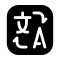
\includegraphics{./images/youtube/_Notes}

\end{column}

\begin{column}{0.001\textwidth}

~

\end{column}

\begin{column}{0.899\textwidth}

\begin{itemize}
\tightlist
\item
  \textbf{Wij zitten in hetzelfde schuitje.} Jedziemy na tym samych wózku. (dosł. Siedzimy w tej samej łódce.)\\
\item
  \textbf{De wasmachine is kapot.} Pralka jest zepsuta.\\
\item
  \textbf{Je verontschuldigt je nu bij je moeder.} Teraz tłumacz się swojej matce.\\
\item
  \textbf{Marek, begrijp me niet verkeerd.} Marek, nie zrozum mnie źle\\
\item
  \textbf{Dat soort religieuze hartstocht is niets voor mij.} Ten rodzaj religijnej pasji jest nie dla mnie.\\
\item
  \textbf{Gewoon verdwijnen, jij en ik.} Po prostu znikajmy, ty i ja.\\
\item
  \textbf{Oké\ldots{} ik hou het voor me.} Okej, zatrzymam to dla siebie.
\end{itemize}

\end{column}

\vfill

\hypertarget{T-smidje}{%
\section{\texorpdfstring{'t Smidje, \emph{Laïs}}{'t Smidje, Laïs}}\label{T-smidje}}

\begin{column}{0.10\textwidth}

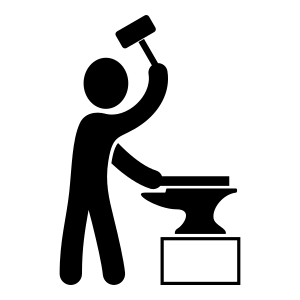
\includegraphics{./images/T-smidje}

\end{column}

\begin{column}{0.04\textwidth}

~

\end{column}

\begin{column}{0.86\textwidth}

\textbf{'t Smidje} \citep{T-smidje} \href{https://youtu.be/mJ6vmtFBlWY}{\includegraphics{./images/youtube/_Youtube}} \emph{Młody kowal} to stara flamandzka piosenka, która stała się popularna w 1998 roku w Hiszpanii i Polsce dzięki grupie Laïs. Stara pisownia z 1848 roku.

\end{column}

\vfill

\begin{column}{0.48\textwidth}

Wie wilt hooren een historie\\
Al van eenen jongen smid\\
Die verbrand had zijn memorie\\
Daeglijks by het vuer verhit\\
Kloppende, kloppende met zijnen hamer\\
Kloppende, kloppende met geweld op zijn aembeld

\end{column}

\begin{column}{0.04\textwidth}

~

\end{column}

\begin{column}{0.48\textwidth}

Kto posłuchać chce historii\\
O pewnym młodym kowalu\\
Który wypalił swoją pamięć\\
Codziennie rozgrzewaną przez ogień\\
Walił, walił swoim młotem\\
Walił z całej siły w swoje kowadło

\end{column}

\vfill\vfill

\begin{column}{0.48\textwidth}

'k Geef den bras van alle het smeden\\
Ik ga naer den franschen zwier\\
'k Wil my tot de trouw begeven\\
'g Hebt nooit schooner vrouw gezien\\
Nimmer meer, nimmer meer met mijnen hamer\\
Nimmer meer, nimmer meer met geweld op mijn aembeld

\end{column}

\begin{column}{0.04\textwidth}

~

\end{column}

\begin{column}{0.48\textwidth}

Rzucam całe to kowalstwo\\
Jadę na francuskie ?salony?\\
Chcę ?udać się? przed ślubem\\
Nikt nie widział piękniejszej kobiety\\
Nigdy więcej, nigdy więcej moim młotem\\
Nigdy więcej z całej siły w moje kowadło

\end{column}

\vfill

\begin{column}{0.48\textwidth}

't Is de schoonste van de vrouwen\\
Maer nooit was er zoo 'n serpent\\
Nooit kan zy heur bakkes houên\\
Nooit is zy eens wel content\\
Was ik nog, was ik nog met mijnen hamer,\\
Was ik nog, was ik nog met geweld op mijn aembeld

\end{column}

\begin{column}{0.04\textwidth}

~

\end{column}

\begin{column}{0.48\textwidth}

Jest najpiękniejsza z wszystkich kobiet\\
Ale nigdy nie było takiej żmii\\
Nigdy nie może się przymknąć\\
Nigdy nie jest zadowolona\\
Czyżbym znowu, czyżbym znowu moim młotem\\
Czyżbym znowu z całej siły w moje kowadło

\end{column}

\vfill

\begin{column}{0.48\textwidth}

Nooit mag ik een pintje drinken\\
Nooit mag ik eens vrolijk zijn\\
Nooit kan ik iemand beschinken\\
Met een glaesje bier of wijn\\
Was ik nog, enz.

\end{column}

\begin{column}{0.04\textwidth}

~

\end{column}

\begin{column}{0.48\textwidth}

Nigdy nie mogę ćwiartki się napić\\
Nigdy nie mogę się trochę zabawić\\
Nigdy nie mogę kogoś poczęstować\\
Szklanką piwa lub wina\\
Czyżbym znowu, itd.

\end{column}

\vfill

\begin{column}{0.48\textwidth}

Wordt er somtijds eens gewasschen\\
Dan moet ik het kind gaê slaen\\
Dan moet ik op 't eten passen\\
Zeep en styfsel halen aen\\
Was ik nog, enz.

\end{column}

\begin{column}{0.04\textwidth}

~

\end{column}

\begin{column}{0.48\textwidth}

Jak jest czasem coś do prania\\
To muszę usypiać dziecko\\
Potem muszę zająć się jedzeniem\\
Mydło i krochmal przyciągnąć\\
Czyżbym znowu, itd.

\end{column}

\vfill

\begin{column}{0.48\textwidth}

Aen de wieg moet zijn gezongen\\
Alles dient tot mijn verdriet\\
Anders greist de kleine jongen\\
Of ik moet zingen een lied\\
Was ik nog, enz.

\end{column}

\begin{column}{0.04\textwidth}

~

\end{column}

\begin{column}{0.48\textwidth}

Nad kołyską musi być zaśpiewane\\
Wszystko w służbie mojemu smutkowi\\
Inaczej ?greist? ten mały chłopiec\\
Albo muszę śpiewać piosenkę\\
Czyżbym znowu, itd.

\end{column}

\vfill

\begin{column}{0.48\textwidth}

'k Geef den bras van al het trouwen\\
Wierd ik maer eens weeuwenaer\\
'k Zou my in een hoeksken houên\\
En my stellen uit gevaer\\
Was ik nog, enz.

\end{column}

\begin{column}{0.04\textwidth}

~

\end{column}

\begin{column}{0.48\textwidth}

Rzucam całe to małżeństwo\\
Gdybym tak kiedyś został wdowcem\\
Skryłbym się w jakimś kąciku\\
I ?wydostałbym? z zagrożenia\\
Czyżbym znowu, itd.

\end{column}

\vfill

\begin{column}{0.10\textwidth}

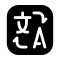
\includegraphics{./images/youtube/_Notes}

\end{column}

\begin{column}{0.001\textwidth}

~

\end{column}

\begin{column}{0.899\textwidth}

\begin{itemize}
\tightlist
\item
  \textbf{Als het monster verhit wordt, stijgt de dampspanning.} Po podgrzaniu próbki wzrasta ciśnienie pary.\\
\item
  \textbf{Adam zat ook voor huiselijk geweld.} Adam siedział też za przemoc domową.\\
\item
  \textbf{Ergens de brui aan geven.} Porzucić coś.\\
\item
  \textbf{Hij gaat aan de zwier met Tomek.} Idzie z Tomkiem włóczyć się po knajpach.\\
\item
  \textbf{Ik moet zich naar huis ter rusten begeven.} Muszę udać się do domu na odpoczynek.\\
\item
  \textbf{Werd ik maar zo gekust.} Gdybym tylko był tak pocałowany. (Gdyby tylko ktoś mnie tak pocałował.)\\
\item
  \textbf{In het Vlaams betekent ``schoon'' mooi.} Po flamandzku „schoon'' znaczy piękny.\\
\item
  \textbf{Misschien niet nu, maar eens wel.} Może nie teraz, ale kiedyś chętnie.\\
\item
  \textbf{Zijn bakkes vangt vliegen.} Dostaje strzała w ryj.\\
\item
  \textbf{Hou je bakkes.} Zamknij się.\\
\item
  \textbf{Jongeren bevrijden zich uit allerlei keurslijven.} Młodzi ludzie uwalniają się od wszelkiego rodzaju kaftanów bezpieczeństwa.
\end{itemize}

\end{column}

\vfill

\hypertarget{Do-rozanca}{%
\chapter{Do różańca}\label{Do-rozanca}}

\begin{column}{0.10\textwidth}

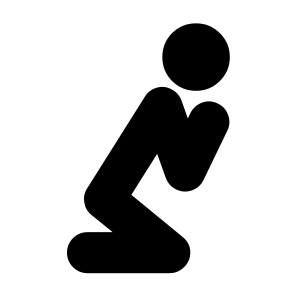
\includegraphics{./images/Do-rozanca}

\end{column}

\begin{column}{0.04\textwidth}

~

\end{column}

\begin{column}{0.86\textwidth}

To są pisoenki do różańca

\end{column}

\vfill

\hypertarget{Afscheid-nemen-bestaat-niet}{%
\section{\texorpdfstring{Afscheid nemen bestaat niet, \emph{Marco Borsato}}{Afscheid nemen bestaat niet, Marco Borsato}}\label{Afscheid-nemen-bestaat-niet}}

\begin{column}{0.10\textwidth}

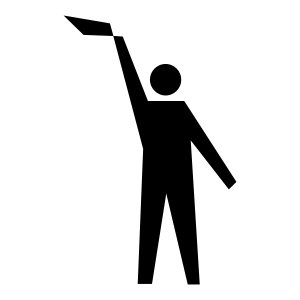
\includegraphics{./images/Afscheid-nemen-bestaat-niet}

\end{column}

\begin{column}{0.04\textwidth}

~

\end{column}

\begin{column}{0.86\textwidth}

\textbf{Afscheid nemen bestaat niet} \citep{Afscheid-nemen-bestaat-niet} \href{https://youtu.be/lSo6LyEA1ks}{\includegraphics{./images/youtube/_Youtube}} \emph{Żegnamy się, nie istnieje} to najpopularniejsza niderlandzkojęzyczna piosenka na pogrzebach.

\end{column}

\vfill

\begin{column}{0.48\textwidth}

Afscheid nemen bestaat niet\\
Ik ga wel weg maar verlaat je niet\\
Mijn lief, je moet me geloven\\
Al doet het pijn

\end{column}

\begin{column}{0.04\textwidth}

~

\end{column}

\begin{column}{0.48\textwidth}

Żegnamy się, nie istnieje\\
Tak, odchodzę, ale cię nie opuszczam\\
Kochanie moje, musisz mi uwierzyć\\
Chociaż to boli

\end{column}

\vfill

\begin{column}{0.48\textwidth}

Ik wil dat je me los laat\\
En dat je morgen weer verder gaat\\
Maar als je eenzaam of bang bent\\
Zal ik er zijn

\end{column}

\begin{column}{0.04\textwidth}

~

\end{column}

\begin{column}{0.48\textwidth}

Chcę, byś pozwoliła mi odejść\\
I byś jutro dalej poszła sama\\
Ale, gdy będziesz samotna lub przestraszona\\
Ja tam będę

\end{column}

\vfill

\begin{column}{0.48\textwidth}

\emph{'k Kom als de wind die je voelt en de regen}\\
\emph{Volg wat je doet als het licht van de maan}\\
\emph{Zoek me in alles dan kom je me tegen}\\
\emph{Fluister mijn naam en ik kom eraan}

\end{column}

\begin{column}{0.04\textwidth}

~

\end{column}

\begin{column}{0.48\textwidth}

\emph{Przychodzę jak wiatr, który czujesz i deszcz}\\
\emph{Podążaj za tym, co robisz jak światło księżyca}\\
\emph{Poszukuj mnie we wszystkim, wtedy mnie spotkasz}\\
\emph{Wyszepcz moje imię, a zaraz tam będę}

\end{column}

\vfill

\begin{column}{0.48\textwidth}

Zie wat onzichtbaar is, wat je gelooft is waar\\
Open je ogen maar en dan zal ik bij je zijn\\
Alles wat jij moet doen is mij op m'n woord geloven\\
Afscheid nemen bestaat niet

\end{column}

\begin{column}{0.04\textwidth}

~

\end{column}

\begin{column}{0.48\textwidth}

Zobacz co niewidzialne, co uważasz za prawdę\\
Otwórz tylko oczy, a ja będę przy tobie\\
Wszystko, co musisz zrobić to uwierzyć mi na słowo\\
Żegnamy się, nie istnieje

\end{column}

\vfill

\begin{column}{0.48\textwidth}

Kijk in de lucht, kijk naar de zee\\
Waar je ook zult lopen, ja, ik loop met je mee\\
Iedere stap en ieder moment\\
waar je dan ook bent

\end{column}

\begin{column}{0.04\textwidth}

~

\end{column}

\begin{column}{0.48\textwidth}

Spójrz w niebo, spójrz na morze\\
Gdziekolwiek pójdziesz, tak, ja pójdę z tobą\\
Z każdym krokiem i w każdej chwili\\
Gdziekolwiek wtedy będziesz

\end{column}

\vfill

\begin{column}{0.48\textwidth}

Wat je ook doet, waar je ook gaat\\
Wanneer je me nodig hebt\\
Fluister gewoon mijn naam en ik kom eraan\\
Afscheid nemen bestaat niet

\end{column}

\begin{column}{0.04\textwidth}

~

\end{column}

\begin{column}{0.48\textwidth}

Cokolwiek będziesz robić, gdziekolwiek pójdziesz\\
Gdy mnie potrzebujesz\\
Po prostu wyszepcz me imię, a zaraz tam będę\\
Żegnamy się, nie istnieje

\end{column}

\vfill

\begin{column}{0.10\textwidth}

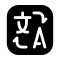
\includegraphics{./images/youtube/_Notes}

\end{column}

\begin{column}{0.001\textwidth}

~

\end{column}

\begin{column}{0.899\textwidth}

\begin{itemize}
\tightlist
\item
  \textbf{En daarom moet ik nu afscheid nemen.} I dlatego muszę się teraz pożegnać.\\
\item
  \textbf{Er bestaat niet één veilige plek meer in Japan.} W Japonii nie ma już bezpiecznego miejsca.\\
\item
  \textbf{Zulke aardige mensen als jou kom je maar zelden tegen.} Rzadko spotykasz tak miłych ludzi jak ty.\\
\item
  \textbf{Ik kan er naartoe, waar je ook wil.} Mogę iść gdziekolwiek chcesz.
\end{itemize}

\end{column}

\vfill

\hypertarget{Klasyka}{%
\chapter{Klasyka}\label{Klasyka}}

\begin{column}{0.10\textwidth}

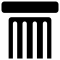
\includegraphics{./images/Klasyka}

\end{column}

\begin{column}{0.04\textwidth}

~

\end{column}

\begin{column}{0.86\textwidth}

Piosenki z list przbojóW

\end{column}

\vfill

\hypertarget{Avond}{%
\section{\texorpdfstring{Avond, \emph{Boudewijn de Groot}}{Avond, Boudewijn de Groot}}\label{Avond}}

\begin{column}{0.10\textwidth}

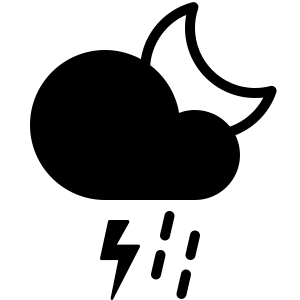
\includegraphics{./images/Avond}

\end{column}

\begin{column}{0.04\textwidth}

~

\end{column}

\begin{column}{0.86\textwidth}

\textbf{Avond} \citep{Avond} \href{https://youtu.be/ptGJ8wzeGDE}{\includegraphics{./images/youtube/_Youtube}} \emph{Wieczór} to piosenka uznawana przez Holendrów za najlepszą niderlandzkojęzyczną piosenkę wszechczasóW.

\end{column}

\vfill

\begin{column}{0.48\textwidth}

Nu hoef je nooit je jas meer aan te trekken\\
En te hopen dat je licht het doet\\
Laat buiten de stormwind nu maar razen in het donker\\
Want binnen is het warm en licht en goed\\
Hand in hand naar buiten kijkend waar de regen valt\\
Ik zie het vuur van hoop en twijfel in je ogen\\
En ik ken je diepste angst

\end{column}

\begin{column}{0.04\textwidth}

~

\end{column}

\begin{column}{0.48\textwidth}

Już nie musisz więcej zakładać kurtki\\
I się martwić, czy zapalą światła\\
Niech na dworze w ciemności szaleje wiatr\\
Bo w środku jest ciepło i widno i dobrze\\
Patrząc na dwór, gdzie pada deszcz trzymam cię za rękę\\
W twoich oczach widzę ogień nadziei i zwątpień\\
I znam twój najgłębszy lęk

\end{column}

\vfill

\begin{column}{0.48\textwidth}

\emph{Want je kunt niets zeker weten en alles gaat voorbij}\\
\emph{Maar ik geloof, ik geloof, ik geloof, ik geloof, ik geloof in jou en mij}

\end{column}

\begin{column}{0.04\textwidth}

~

\end{column}

\begin{column}{0.48\textwidth}

\emph{Bo niczego nie możesz być pewna, a wszystko przemija}\\
\emph{Ale wierzę, wierzę, wierzę, wierzę, wierzę w ciebie i we mnie}

\end{column}

\vfill

\begin{column}{0.48\textwidth}

En als je 's morgens opstaat ben ik bij je\\
En misschien heb ik al thee gezet\\
En als de zon schijnt buiten gaan we lopen door de duinen\\
En als het regent gaan we t'rug in bed\\
Uren langzaam wakker worden, zwevend door de tijd\\
Ik zie het licht door de gordijnen\\
En ik weet, t'verleden geeft geen zekerheid

\end{column}

\begin{column}{0.04\textwidth}

~

\end{column}

\begin{column}{0.48\textwidth}

A kiedy wstaniesz rano, to ja będę przy tobie\\
I może herbata już będzie zrobiona\\
I jeśli na dworze będzie słonecznie, to pójdziemy na wydmy\\
A gdyby padało, to wrócimy do łóżka\\
Godziny powoli się budzą unosząc się w czasie\\
Widzę światło przez zasłony\\
I wiem, że przeszłość nie daje pewności

\end{column}

\vfill

\begin{column}{0.48\textwidth}

Ik doe de lichten uit en de kamer wordt nu donker\\
Een straatlantaarn buiten geeft wat licht\\
En de dingen in de kamer worden vrienden die gaan slapen\\
De stoelen staan te wachten op 't ontbijt\\
En morgen wordt ik wakker met de geur van brood en honing\\
De glans van gouden zonlicht in je haar\\
En de dingen in de kamer, ik zeg ze welterusten\\
Vanavond gaan we slapen en morgen zien we wel\\
Maar de dingen in de kamer zouden levenloze dingen zijn\\
Zonder jou

\end{column}

\begin{column}{0.04\textwidth}

~

\end{column}

\begin{column}{0.48\textwidth}

Gaszę światło i teraz w pokoju robi się ciemniej\\
Latarnia na ulicy daje nieco światła\\
A rzeczy w pokoju stają się przyjaciółmi, którzy idą spać\\
Krzesła oczekują na śniadanie\\
A jutro obudzę się z zapachem chleba i miodu\\
Błysk złotych promieni słońca w twoich włosach\\
A rzeczą w pokoju, mówię dobranoc\\
Dzisiaj pójdziemy spać i zobaczymy się znowu jutro\\
Ale rzeczy w pokoju byłyby martwe\\
Bez ciebie

\end{column}

\vfill

\begin{column}{0.10\textwidth}

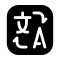
\includegraphics{./images/youtube/_Notes}

\end{column}

\begin{column}{0.001\textwidth}

~

\end{column}

\begin{column}{0.899\textwidth}

\begin{itemize}
\tightlist
\item
  \textbf{Doe het licht maar uit.} Po prostu wyłącz światło.\\
\item
  \textbf{Ik wil je nooit meer zien.} Nie chcę cię nigdy więcej widzieć.\\
\item
  \textbf{Ze liepen hand in hand.} Szli trzymając się za ręce.\\
\item
  \textbf{Die jongen toonde geen angst.} Ten chłopiec nie okazywał strachu.\\
\item
  \textbf{Het is te hopen dat \ldots{}} Należy mieć nadzieją, że \ldots{}\\
\item
  \textbf{De vlam zweeft vaak net boven het hout.} Płomień unosi się często tuż nad drewnem.\\
\item
  \textbf{Ga Maria wakker maken.} Idź obudź Marię\\
\item
  \textbf{Ik sta op het punt uit te gaan.} Zaraz wychodzę.\\
\item
  \textbf{De geur van lelies vulde de kamer.} Zapach lilii wypełnił pokój.\\
\item
  \textbf{De glans wordt gemeten volgens ISO 2813.} Połysk mierzy się zgodnie z ISO 2813.\\
\item
  \textbf{Ik zie je wel bij de auto.} Do zobaczenia w aucie.
\end{itemize}

\end{column}

\vfill

\hypertarget{Blauwe-dag}{%
\section{\texorpdfstring{Blauwe Dag, \emph{Suzan \& Freek}}{Blauwe Dag, Suzan \& Freek}}\label{Blauwe-dag}}

\begin{column}{0.10\textwidth}

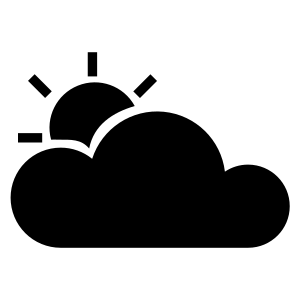
\includegraphics{./images/Blauwe-dag}

\end{column}

\begin{column}{0.04\textwidth}

~

\end{column}

\begin{column}{0.86\textwidth}

\textbf{Blauwe Dag} \citep{Blauwe-dag} \href{https://youtu.be/keYF1D0LVQk}{\includegraphics{./images/youtube/_Youtube}} \emph{Gorszy Dzień} \ldots\ldots.. .

\end{column}

\vfill

\begin{column}{0.48\textwidth}

Weet je nog dat jij me zei dat wij nooit zouden vluchten als een van ons\\
Loopt door de regen en nooit meer kijkt naar hoe het leven is in de zon\\
Weet je nog dat jij me zei dat jij d'r altijd bent als ik je nodig heb\\
Nee, ik ben het niet vergeten, nee\\
Wat jij me ooit hebt gezegd

\end{column}

\begin{column}{0.04\textwidth}

~

\end{column}

\begin{column}{0.48\textwidth}

Czy pamiętasz, jak mi powiedziałaś, że nie ucieklibyśmy nigdy, gdyby któreś z nas\\
Szło przez deszcz i już nigdy więcej nie oglądało tego, jak wygląda życie w słońcu\\
Czy pamiętasz, jak mi powiedziałaś, że jesteś zawsze przy mnie, gdy cię potrzebuję\\
Nie, ja tego nie zapomniałam, nie\\
Co mi kiedyś powiedziałeś

\end{column}

\vfill

\begin{column}{0.48\textwidth}

Want ik zie dat jij het moeilijk hebt en niet meer lachen kan zoals je vroeger deed\\
En nauwelijks in de gaten hebt dat je anders loopt dan dat je deed voorheen\\
Weet je nog dat jij me zei dat jij d'r altijd bent als ik je nodig heb\\
Nee, ik ben het niet vergeten, nee\\
Wat jij me ooit hebt gezegd

\end{column}

\begin{column}{0.04\textwidth}

~

\end{column}

\begin{column}{0.48\textwidth}

Bo widzę, że masz trudności i nie możesz się już śmiać, tak jak kiedyś\\
I ledwo zauważasz, że chodzisz inaczej niż to kiedyś robiłeś\\
Czy pamiętasz, jak mi powiedziałaś, że jesteś zawsze przy mnie, gdy cię potrzebuję\\
Nie, ja tego nie zapomniałam, nie\\
Co mi kiedyś powiedziałeś

\end{column}

\vfill

\begin{column}{0.48\textwidth}

\emph{Blauwe dag, als het dondert}\\
\emph{En valt de hemel naar beneden, ben ik hier bij jou alleen}\\
\emph{Blauwe dag, een seconde}\\
\emph{Laten we dansen tot de morgen en de lucht weer opengaat}

\end{column}

\begin{column}{0.04\textwidth}

~

\end{column}

\begin{column}{0.48\textwidth}

\emph{Gorszy dzień, kiedy grzmi}\\
\emph{I niebo spada w dół, jestem tu z tobą sam na sam}\\
\emph{Gorszy dzień, jedna sekunda}\\
\emph{Tańczmy do rana, a niebo znów się przejaśni}

\end{column}

\vfill

\begin{column}{0.48\textwidth}

\emph{Fiets met jou mee door heel de stad}\\
\emph{Als jij dat wil, nou, dan doe ik dat. Ik ben hier op je blauwe dag}\\
\emph{Blauwe dag, een seconde}\\
\emph{Laten we dansen tot de morgen en de lucht weer opengaat}

\end{column}

\begin{column}{0.04\textwidth}

~

\end{column}

\begin{column}{0.48\textwidth}

\emph{Pojechać z tobą na rowerze przez całe miasto}\\
\emph{Jeśli tego chcesz, teraz, to to zrobię. Jestem tu w twój gorszy dzień}\\
\emph{Gorszy dzień, jedna sekunda}\\
\emph{Tańczmy do rana, a niebo znów się przejaśni}

\end{column}

\vfill

\begin{column}{0.48\textwidth}

Weet je nog dat jij me zei dat jij d'r altijd bent wanneer ik ergens val\\
Nu lig ik zelf op de grond en ben ik diegene zonder licht in een donker dal\\
Ik ging van de top van de wereld naar de plek waar ik niemand ken\\
Nee, ik ben het niet vergeten, nee\\
Wat jij me ooit hebt gezegd

\end{column}

\begin{column}{0.04\textwidth}

~

\end{column}

\begin{column}{0.48\textwidth}

Czy pamiętasz, jak mi powiedziałaś, że jesteś zawsze przy mnie, gdy upadam\\
Teraz leżę na ziemi i jestem tu bez światła w jakiejś ciemnej dolinie\\
Zszedłem ze szczytu świata do miejsca, w którym nikogo nie znam\\
Nie, ja tego nie zapomniałam, nie\\
Co mi kiedyś powiedziałeś

\end{column}

\vfill

\begin{column}{0.10\textwidth}

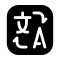
\includegraphics{./images/youtube/_Notes}

\end{column}

\begin{column}{0.001\textwidth}

~

\end{column}

\begin{column}{0.899\textwidth}

\begin{itemize}
\tightlist
\item
  \textbf{De lucht wordt donker.} Niebo robi się ciemne.\\
\item
  \textbf{De lucht klaarde op.} Niebo się przejaśniło.\\
\item
  \textbf{De hemel is blauw} Niebo jest niebieskie.\\
\item
  \textbf{Zijn ziel was in het hemel} Jego dusza była w niebie.\\
\item
  \textbf{Ik voel me blauw.} Jestem przygnębiony.\\
\item
  \textbf{Weet je nog?} Czy pamiętasz?\\
\item
  \textbf{Laten we haar alleen laten.} Zostawmy ją w spokoju.\\
\item
  \textbf{Ik denk dat wij goede vrienden zouden kunnen zijn.} Myślę, że moglibyśmy być dobrymi przyjaciółmi.\\
\item
  \textbf{Hij kan nauwelijks lezen.} On ledwo umie czytać.\\
\item
  \textbf{Houd deze koffer in de gaten.} Obserwuj tę walizkę.
\end{itemize}

\end{column}

\vfill

\hypertarget{Brabant}{%
\section{\texorpdfstring{Brabant, \emph{Guus Meeuwis}}{Brabant, Guus Meeuwis}}\label{Brabant}}

\begin{column}{0.10\textwidth}

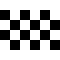
\includegraphics{./images/Brabant}

\end{column}

\begin{column}{0.04\textwidth}

~

\end{column}

\begin{column}{0.86\textwidth}

\textbf{Brabant} \citep{Brabant} \href{https://youtu.be/YaIzl1Tz-so}{\includegraphics{./images/youtube/_Youtube}} \emph{Brabancja} to nieoficjalny hymn Brabancji Północnej, który powstał w Moskwie.

\end{column}

\vfill

\begin{column}{0.48\textwidth}

Een muts op mijn hoofd, mijn kraag staat omhoog\\
Het is hier ijskoud, maar gelukkig wel droog

\end{column}

\begin{column}{0.04\textwidth}

~

\end{column}

\begin{column}{0.48\textwidth}

Czapka na mojej głowie, mój kołnierz stoi do góry\\
Jest mroźno ale na szczęście sucho

\end{column}

\vfill

\begin{column}{0.48\textwidth}

De dagen zijn kort hier, de nacht begint vroeg\\
De mensen zijn stug, en er is maar één kroeg

\end{column}

\begin{column}{0.04\textwidth}

~

\end{column}

\begin{column}{0.48\textwidth}

Dni są tutaj krótkie, noc zaczyna się wcześnie\\
Ludzie są sztywni i jest tylko jeden pub

\end{column}

\vfill

\begin{column}{0.48\textwidth}

Als ik naar mijn hotel loop, na een donkere dag,\\
Dan voel ik mijn huissleutel diep in mijn zak

\end{column}

\begin{column}{0.04\textwidth}

~

\end{column}

\begin{column}{0.48\textwidth}

Gdy idę do mojego hotelu po ciemnym dniu\\
Głęboko w kieszeni wyczuwam klucz do domu

\end{column}

\vfill

\begin{column}{0.48\textwidth}

\emph{Ik loop hier alleen in een te stille stad}\\
\emph{Ik heb eigenlijk nooit last van heimwee gehad}\\
\emph{Maar de mensen ze slapen, de wereld gaat dicht}\\
\emph{En dan denk ik aan Brabant, want daar brandt nog licht}

\end{column}

\begin{column}{0.04\textwidth}

~

\end{column}

\begin{column}{0.48\textwidth}

\emph{Idę tu sam w zbyt cichym mieście}\\
\emph{Tak naprawdę nigdy nie tęskniłem za domem}\\
\emph{Ale ludzie, oni śpią, świat się zamyka}\\
\emph{I wtedy myślę o Brabancji bo tam wciąż pali się światło}

\end{column}

\vfill

\begin{column}{0.48\textwidth}

Ik mis hier de warmte van een dorpscafé,\\
De aanspraak van mensen met een zachte G

\end{column}

\begin{column}{0.04\textwidth}

~

\end{column}

\begin{column}{0.48\textwidth}

Tutaj tęsknię za ciepłem wiejskiej kawiarni\\
Za kontaktem z ludźmi o miękkim G

\end{column}

\vfill

\begin{column}{0.48\textwidth}

Ik mis zelfs het zeiken, op alles om niets\\
Was men maar op Brabant zo trots als een Fries

\end{column}

\begin{column}{0.04\textwidth}

~

\end{column}

\begin{column}{0.48\textwidth}

Tęsknię nawet za narzekaniem na wszystko bez powodu\\
Gdyby tylko Brabantczyk był tak dumny jak jest Fryzyjczyk

\end{column}

\vfill

\begin{column}{0.48\textwidth}

In het zuiden vol zon woon ik samen met jou\\
't Is daarom dat ik zo van Brabanders houd

\end{column}

\begin{column}{0.04\textwidth}

~

\end{column}

\begin{column}{0.48\textwidth}

Mieszkam razem z tobą na południu pełnym słońca\\
Dlatego tak bardzo kocham Brabantczyków

\end{column}

\vfill

\begin{column}{0.48\textwidth}

De Peel en de Kempen en de Meierij,\\
Maar het mooiste aan Brabant ben jij, dat ben jij

\end{column}

\begin{column}{0.04\textwidth}

~

\end{column}

\begin{column}{0.48\textwidth}

Peel i Kempen i Meierij są piękne\\
Ale najpiękniejsza w Brabancji jesteś ty, to jesteś ty

\end{column}

\vfill

\begin{column}{0.10\textwidth}

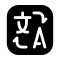
\includegraphics{./images/youtube/_Notes}

\end{column}

\begin{column}{0.001\textwidth}

~

\end{column}

\begin{column}{0.899\textwidth}

\begin{itemize}
\tightlist
\item
  \textbf{Als je niets te zeggen hebt, zeg dan niets., Jeśli nie masz nic do powiedzenia nic nie mów.}NA\\
\item
  \textbf{Ze is net zo bezig als Tomek.} Jest tak samo zajęta jak Tomek.\\
\item
  \textbf{De Peel, De Kempen en De Meierij zijn de mooiste plekken van Brabant.} Peel, Kempen i Meierij to najpiękniejsze miejsca w Brabancji.
\end{itemize}

\end{column}

\vfill

\hypertarget{Dromen-zijn-bedrog}{%
\section{\texorpdfstring{Dromen zijn bedrog, \emph{Marco Borsato}}{Dromen zijn bedrog, Marco Borsato}}\label{Dromen-zijn-bedrog}}

\begin{column}{0.10\textwidth}

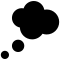
\includegraphics{./images/Dromen-zijn-bedrog}

\end{column}

\begin{column}{0.04\textwidth}

~

\end{column}

\begin{column}{0.86\textwidth}

\textbf{Dromen zijn bedrog} \citep{Dromen-zijn-bedrog} \href{https://youtu.be/CuA2U9iU6lQ}{\includegraphics{./images/youtube/_Youtube}} \emph{Sny są ulotne} jest uważana za jeden z najbardziej udanych singli w języku niderlandzkim wszech czasów.

\end{column}

\vfill

\begin{column}{0.48\textwidth}

Steeds als ik je zie lopen dan gaat de hemel een klein beetje open\\
Sterren, je laat ze verbleken met je ogen die altijd stralen\\
Jij kan de zon laten schijnen want je loopt langs en de wolken verdwijnen en als je lacht, lacht heel de wereld mee

\end{column}

\begin{column}{0.04\textwidth}

~

\end{column}

\begin{column}{0.48\textwidth}

Zawsze, kiedy widzę jak idziesz, wtedy odrobinę otwiera się niebo\\
Gwiazdy, sprawiasz że one bledną, swoimi oczami, które cały czas promienieją\\
Możesz pozwolić słońcu świecić, bo gdy przechodzisz chmury znikają a kiedy się śmiejesz, razem śmieje się cały świat

\end{column}

\vfill

\begin{column}{0.48\textwidth}

\emph{De meeste dromen zijn bedrog maar als ik wakker word naast jou dan droom ik nog}\\
\emph{Ik voel je adem en zie je gezicht je bent een droom die naast me ligt}\\
\emph{Je kijkt me aan en rekt je uit een keer in de zoveel tijd komen dromen uit!}

\end{column}

\begin{column}{0.04\textwidth}

~

\end{column}

\begin{column}{0.48\textwidth}

\emph{Najczęściej sny są ulotne, ale kiedy budzę się obok ciebie, wciąż marzę}\\
\emph{Czuję twój oddech i widzę twoją twarz, jesteś snem leżącym obok mnie}\\
\emph{Patrzysz na mnie i się wyciągasz raz na jakiś czas marzenia się spełniają!}

\end{column}

\vfill

\begin{column}{0.48\textwidth}

Jij moet me een ding beloven laat me nog lang in mijn dromen geloven\\
Zelfs als je even niet hier bent blijf in mijn slaap dan bij me\\
En als de zon weer gaat schijnen laat dan dat beeld wat ik heb niet verdwijnen. Als je zou gaan, neem je mijn dromen mee

\end{column}

\begin{column}{0.04\textwidth}

~

\end{column}

\begin{column}{0.48\textwidth}

Musisz mi obiecać jedno, pozwól mi jeszcze długo wierzyć w moje marzenia\\
Nawet jeśli cię chwilę tutaj nie ma, zostań ze mną kiedy śpię\\
A kiedy znów zaświeci słońce, nie pozwól fantazji którą mam zniknąć. Gdybyś szła, zabierz ze sobą moje marzenia

\end{column}

\vfill

\begin{column}{0.10\textwidth}

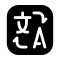
\includegraphics{./images/youtube/_Notes}

\end{column}

\begin{column}{0.001\textwidth}

~

\end{column}

\begin{column}{0.899\textwidth}

\begin{itemize}
\tightlist
\item
  \textbf{Dromen zijn bedrog.} Sen mara, Bóg wiara. {[}prov. za Czochralski{]}\\
\item
  \textbf{Met een klein beetje geluk.} Przy odrobinie szczęścia.\\
\item
  \textbf{De deur gaat niet open, hij klemt.} Drzwi się nie otwierają, są zablokowane.\\
\item
  \textbf{Kom met me mee.} Chodź razem ze mną.\\
\item
  \textbf{Als ik vragen mag.} Jeśli wolno spytać.\\
\item
  \textbf{Ik reik mijn hand naar je uit.} Wyciągam rękę do ciebie.\\
\item
  \textbf{De narcissen kwamen uit.} Wypuściły żonkile.\\
\item
  \textbf{Een keer in de zoveel tijd.} Raz na jakiś czas.\\
\item
  \textbf{Mag ik even binnenkomen?} Czy mogę na chwilę wejść?\\
\item
  \textbf{Ik blijf in slaap vallen.} Ciągle zasypiam.\\
\item
  \textbf{Wat heb je vannacht gedroomd?} Co ci się śniło dzisiaj w nocy?\\
\item
  \textbf{Waar droom je over?} O czym marzysz?
\end{itemize}

\end{column}

\vfill

\hypertarget{Duurt-te-lang}{%
\section{\texorpdfstring{Duurt Te Lang, \emph{Davina Michelle}}{Duurt Te Lang, Davina Michelle}}\label{Duurt-te-lang}}

\begin{column}{0.10\textwidth}

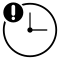
\includegraphics{./images/Duurt-te-lang}

\end{column}

\begin{column}{0.04\textwidth}

~

\end{column}

\begin{column}{0.86\textwidth}

\textbf{Duurt Te Lang} \citep{Duurt-te-lang} \href{https://youtu.be/n_j1clPqEvg}{\includegraphics{./images/youtube/_Youtube}} \emph{To trwa zbyt długo} to numer, który czekał 5 lat na nowego wykonawcę i stanie się hitem.

\end{column}

\vfill

\begin{column}{0.48\textwidth}

We konden over alles praten, alles\\
Maar alles ging over de liefde, we vergaten alles\\
In een brief, een smsje, in een liedje schreef ik\\
Ik zal alles voor je doen en voor je liefde leef ik

\end{column}

\begin{column}{0.04\textwidth}

~

\end{column}

\begin{column}{0.48\textwidth}

Mogliśmy rozmawiać o wszystkim, o wszystkim\\
Ale wszystko poszło o miłość, zapomnieliśmy wszystko\\
Napisałem w liście, SMS-ie, w piosence\\
Zrobię dla ciebie wszystko i żyję dla twojej miłości

\end{column}

\vfill

\begin{column}{0.48\textwidth}

En die liefde kreeg ik en vaak in overmaten\\
Je kon de drempels van het leven aan mij overlaten\\
Je zag die meiden haten want je had je superheld\\
Ik had m'n vrienden net te vaak over jou verteld

\end{column}

\begin{column}{0.04\textwidth}

~

\end{column}

\begin{column}{0.48\textwidth}

I dostałem tę miłość, i często z nadmiarem\\
Przeszkody życiowe mogłaś pozostawić mi\\
Widziałeś nienawidzące dziewczyny, bo ty miałaś swego superbohatera\\
Opowiadałem mojej sieci przyjaciół zbyt często o tobie

\end{column}

\vfill

\begin{column}{0.48\textwidth}

Nu staren we samen naar de tafel, met de mondjes dicht\\
Met blikken die vanzelf spreken, in ons gezicht\\
Ik heb het overgrote deel van alles aangericht\\
Maar ik rijd te lang in deze tunnel en ik zie geen licht

\end{column}

\begin{column}{0.04\textwidth}

~

\end{column}

\begin{column}{0.48\textwidth}

Teraz wpatrujemy się razem w stół z zamkniętymi ustami\\
Ze spojrzeniami, które mówią same za siebie, w nasze twarze\\
Spowodowałem zdecydowaną większość tego wszystkiego\\
Ale jadę w tym tunelu zbyt długo i nie widzę światła

\end{column}

\vfill

\begin{column}{0.48\textwidth}

Dus doe je ogen dicht voor onze laatste zet\\
En denk terug aan het kleine huisje met het kleine bed\\
Shit, maar morgen is de pijn terug\\
Staan we uren op de halte, rijdt een trein terug

\end{column}

\begin{column}{0.04\textwidth}

~

\end{column}

\begin{column}{0.48\textwidth}

Więc zamknij oczy przed naszym ostatnim posunięciem\\
I wróć myślami do małego domku z małym łóżkiem\\
Cholera, ale ból wróci jutro\\
Będziemy stać godzinami na przystanku, pociąg pojedzie z powrotem

\end{column}

\vfill

\begin{column}{0.48\textwidth}

\emph{Het duurt te lang}\\
\emph{We staan hier al een tijdje}\\
\emph{En we moeten door, dus voor de laatste keer het spijt me}\\
\emph{Het duurt te lang}

\end{column}

\begin{column}{0.04\textwidth}

~

\end{column}

\begin{column}{0.48\textwidth}

\emph{To trwa zbyt długo}\\
\emph{Stoimy tu już jakiś czas}\\
\emph{Musimy do przodu, więc po raz ostatni wybacz mi}\\
\emph{To trwa zbyt długo}

\end{column}

\vfill

\begin{column}{0.48\textwidth}

\emph{Het duurt te lang}\\
\emph{We staan stil}\\
\emph{Wat jij wil, wat ik wil}\\
\emph{Het duurt te lang}

\end{column}

\begin{column}{0.04\textwidth}

~

\end{column}

\begin{column}{0.48\textwidth}

\emph{To trwa zbyt długo}\\
\emph{Stoimy w miejscu}\\
\emph{Czego chcesz ty, czego chcę ja}\\
\emph{To trwa zbyt długo}

\end{column}

\vfill

\begin{column}{0.48\textwidth}

Twee stille mensen aan de tafel, het is geen gezicht\\
Ik kan die route niet belopen met m'n ogen dicht\\
Je weet precies wat ik ga zeggen, ik weet het ook van jou\\
En op het eind vertel ik vast hoeveel ik van je hou

\end{column}

\begin{column}{0.04\textwidth}

~

\end{column}

\begin{column}{0.48\textwidth}

Dwoje milczących ludzi przy stole bez twarzy\\
Nie mogę iść dalej tą drogą z zamkniętymi oczami\\
Wiesz dokładnie, co powiem, ja wiem co powiesz ty\\
A na koniec powiem ci na pewno, jak bardzo cię kocham

\end{column}

\vfill

\begin{column}{0.48\textwidth}

En daarna slaan de deuren weer, en breekt er weer een glas\\
Daarna valt er weer een traan, en pak ik weer m'n tas\\
En daarna hou ik je weer stevig vast\\
En leg me kleren weer terug in de kast

\end{column}

\begin{column}{0.04\textwidth}

~

\end{column}

\begin{column}{0.48\textwidth}

A potem znów trzaskają drzwi i kolejna pęka szyba\\
Potem leci kolejna łza i znów biorę torbę\\
A potem na pewno znowu bardzo mocno cię tulę\\
I znowu wkładam swoje ubrania z powrotem do szafy

\end{column}

\vfill

\begin{column}{0.48\textwidth}

Dus, ik hou je nog een poosje vast\\
Want dan vergeet je nog hoe boos je was\\
Maar de pijn blijft zitten, dus het helpt niet\\
Dus waarschijnlijk is het morgen weer hetzelfde lied

\end{column}

\begin{column}{0.04\textwidth}

~

\end{column}

\begin{column}{0.48\textwidth}

Więc zatrzymam cię jeszcze na chwilkę na pewno\\
Bo wtedy jeszcze zapomnisz jak byłaś zła\\
Ale ból pozostaje w środku, więc to nie pomaga\\
Więc pewnie jutro od nowa ta sama piosenka

\end{column}

\vfill

\begin{column}{0.48\textwidth}

De tekst komt op hetzelfde neer in dezelfde beat\\
Een soort van gouden verf op een blok verdriet\\
Conflicten zijn normaal, maar het moet ons niet verstikken\\
Me tranen vallen nu, dus ik laat het liedje snikken

\end{column}

\begin{column}{0.04\textwidth}

~

\end{column}

\begin{column}{0.48\textwidth}

Tekst chodzi tak samo w górę jak i w dół w tym samym rytmie\\
Jakiś rodzaj złotej farby na bloku smutku\\
Konflikty są normalne, ale nie powinny nas dusić\\
Moje łzy nie lecą, więc pozwalam tej piosence szlochać

\end{column}

\vfill

\begin{column}{0.10\textwidth}

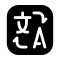
\includegraphics{./images/youtube/_Notes}

\end{column}

\begin{column}{0.001\textwidth}

~

\end{column}

\begin{column}{0.899\textwidth}

\begin{itemize}
\tightlist
\item
  \textbf{Misschien moet je de diagnose aan mij overlaten.} Być może powinieneś diagnozę pozostawić mi.\\
\item
  \textbf{Hij heeft deze schade aangericht.} On wyrządził te szkody.\\
\item
  \textbf{Onze kosten belopen circa 1 miljoen PLN.} Nasze koszty wynoszą około 1 milion złotych.\\
\item
  \textbf{Je bent al een poos binnen.} Jesteś w środku już przez jakiś czas.\\
\item
  \textbf{Beweeg je vingers langzaam op en neer.} Powoli przesuwaj palce w górę i w dół.
\end{itemize}

\end{column}

\vfill

\hypertarget{Een-beetje-verliefd}{%
\section{\texorpdfstring{Een beetje verliefd, \emph{André Hazes}}{Een beetje verliefd, André Hazes}}\label{Een-beetje-verliefd}}

\begin{column}{0.10\textwidth}

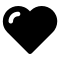
\includegraphics{./images/Een-beetje-verliefd}

\end{column}

\begin{column}{0.04\textwidth}

~

\end{column}

\begin{column}{0.86\textwidth}

\textbf{Een beetje verliefd} \citep{Een-beetje-verliefd} \href{https://youtu.be/3kufNNxyACg}{\includegraphics{./images/youtube/_Youtube}} \emph{Trochę zakochany} to piosenka o niespełnionej miłości Rozpoczyna się w scenerii podobnej do tej z piosenki \ref{Leef} wykonanej przez syna André Hazes jr.

\end{column}

\vfill

\begin{column}{0.48\textwidth}

In een discotheek, zat ik van de week\\
En ik voelde mij daar zo alleen\\
't Was er warm en druk, ik zat naast een lege kruk\\
Ik verlangde zo naar jou hier aan m'n zij

\end{column}

\begin{column}{0.04\textwidth}

~

\end{column}

\begin{column}{0.48\textwidth}

W jakiejś dyskotece byłem na tygodniu\\
I czułem się tam bardzo samotny\\
Było tam gorąco i tłoczno, siedziałem przy pustym stołku\\
Tak pragnąłem cię tutaj przy moim boku

\end{column}

\vfill

\begin{column}{0.48\textwidth}

Ja, ik denk nog steeds hoe het was geweest\\
Toen je naast me zat hier aan de bar\\
Ik vroeg: `'Drink je mee?'', dat vond jij oké\\
Toen je proostend naar me keek werd ik zo week

\end{column}

\begin{column}{0.04\textwidth}

~

\end{column}

\begin{column}{0.48\textwidth}

Tak, wciąż się zastanawiam, jak to było\\
Gdy się do mnie przysiadłaś przy barze\\
Spytałem: `'Napijesz się ze mną?'', zgodziłaś się\\
Kiedy na mnie spojrzałaś przy toaście, stałem się taki miękki

\end{column}

\vfill

\begin{column}{0.48\textwidth}

\emph{Een beetje verliefd, ik dacht een beetje verliefd}\\
\emph{Als ik wist wat jij toen dacht, had ik nooit op jou gewacht}\\
\emph{Als een kind zat ik te dromen deze nacht ben jij voor mij}\\
\emph{Maar die droom ging snel voorbij}

\end{column}

\begin{column}{0.04\textwidth}

~

\end{column}

\begin{column}{0.48\textwidth}

\emph{Trochę zakochany, myślałem trochę zakochany}\\
\emph{Gdybym wiedział, co wtedy myślisz, nigdy bym na ciebie nie czekał}\\
\emph{Jak małe dziecko ciągle marzyłem, tej nocy jesteś dla mnie}\\
\emph{Ale ten sen szybko minął}

\end{column}

\vfill

\begin{column}{0.48\textwidth}

Jij stond op en zei: `'Hou m'n plaatsje vrij\\
Ik moet even weg maar ben zo terug''\\
Ach, die kruk bleef leeg tot ik in de gaten kreeg\\
Dat je wegging zonder mij, ik was nu alleen

\end{column}

\begin{column}{0.04\textwidth}

~

\end{column}

\begin{column}{0.48\textwidth}

Wstałaś i powiedziałaś: `'Zajmij mi miejsce\\
Muszę na chwilę wyjść, ale zaraz wrócę''\\
Ach, ten stołek stał pusty, dopóki nie zauważyłem\\
Że odeszłaś beze mnie, teraz byłem sam

\end{column}

\vfill

\begin{column}{0.10\textwidth}

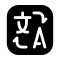
\includegraphics{./images/youtube/_Notes}

\end{column}

\begin{column}{0.001\textwidth}

~

\end{column}

\begin{column}{0.899\textwidth}

\begin{itemize}
\tightlist
\item
  \textbf{Weet je wat, ik ben er zat van.} Wiesz co, mam tego dosyć.\\
\item
  \textbf{Ik verlang ernaar met je alleen te zijn.} Pragnę być z tobą sam.\\
\item
  \textbf{Ik heb de wet aan m'n zij(-de).} Prawo mam po swojej stronie.\\
\item
  \textbf{Dat vind ik erg leuk.} To mi się bardzo podoba.\\
\item
  \textbf{We zitten te praten.} Gadamy sobie.\\
\item
  \textbf{Ik krijg dit in de gaten.} Zdaję sobie sprawę z tego
\end{itemize}

\end{column}

\vfill

\hypertarget{Het-dorp}{%
\section{\texorpdfstring{Het dorp, \emph{Wim Sonneveld}}{Het dorp, Wim Sonneveld}}\label{Het-dorp}}

\begin{column}{0.10\textwidth}

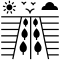
\includegraphics{./images/Het-dorp}

\end{column}

\begin{column}{0.04\textwidth}

~

\end{column}

\begin{column}{0.86\textwidth}

\textbf{Het dorp} \citep{Het-dorp} \href{https://youtu.be/C8Ff5OEUzd8}{\includegraphics{./images/youtube/_Youtube}} \emph{Wieś} to wspomnienia autora tekstu o utraconym dzieciństwie. Hugo Verhage to naprawdę Friso Wiegersma. Z wykonawcą piosenki Wimem Sonneveld byli w związku. .

\end{column}

\vfill

\begin{column}{0.48\textwidth}

Thuis heb ik nog een ansichtkaart\\
Waarop een kerk een kar met paard\\
Een slagerij J. van der Ven\\
Een kroeg, een juffrouw op de fiets

\end{column}

\begin{column}{0.04\textwidth}

~

\end{column}

\begin{column}{0.48\textwidth}

W domu wciąż mam pocztówkę\\
Na niej kościół i koń z wozem\\
Sklep mięsny J. van der Ven\\
Pub, dziewczyna na rowerze

\end{column}

\vfill

\begin{column}{0.48\textwidth}

Het zegt u hoogstwaarschijnlijk niets\\
Maar het is waar ik geboren ben\\
Dit dorp, ik weet nog hoe het was\\
De boerenkind'ren in de klas

\end{column}

\begin{column}{0.04\textwidth}

~

\end{column}

\begin{column}{0.48\textwidth}

Pewnie nic ci to nie mówi\\
Ale tam się urodziłem\\
Ta wieś, wciąż pamiętam jak to było\\
Wiejskie dzieci w klasie

\end{column}

\vfill

\begin{column}{0.48\textwidth}

Een kar die ratelt op de keien\\
Het raadhuis met een pomp ervoor\\
Een zandweg tussen koren door\\
Het vee, de boerderijen

\end{column}

\begin{column}{0.04\textwidth}

~

\end{column}

\begin{column}{0.48\textwidth}

Wóz klekocze na kamieniach\\
Ratusz z pompą przed nim\\
Polna droga wśród pszenicy hen\\
Żywy inwentarz, zagrody chłopskie

\end{column}

\vfill

\begin{column}{0.48\textwidth}

\emph{En langs het tuinpad van m'n vader}\\
\emph{Zag ik de hoge bomen staan}\\
\emph{Ik was een kind en wist niet beter}\\
\emph{Dan dat 't nooit voorbij zou gaan}

\end{column}

\begin{column}{0.04\textwidth}

~

\end{column}

\begin{column}{0.48\textwidth}

\emph{I wzdłuż ścieżki w ogrodzie ojca}\\
\emph{Widziałem jak rosną wysokie drzewa}\\
\emph{Byłem dzieckiem i wiedziałem na pewno}\\
\emph{Że to nigdy nie przeminie}

\end{column}

\vfill

\begin{column}{0.48\textwidth}

Wat leefden ze eenvoudig toen\\
In simp'le huizen tussen groen\\
Met boerenbloemen en een heg\\
Maar blijkbaar leefden ze verkeerd

\end{column}

\begin{column}{0.04\textwidth}

~

\end{column}

\begin{column}{0.48\textwidth}

Jakże wtedy żyli zwyczajnie\\
W prostych domach wśród zieleni\\
Z polnymi/wiejskimi kwiatami i żywopłotem\\
Ale widocznie żyli niewłaściwie

\end{column}

\vfill

\begin{column}{0.48\textwidth}

Het dorp is gemoderniseerd\\
En nou zijn ze op de goeie weg\\
Want ziet, hoe rijk het leven is\\
Ze zien de televisiequiz

\end{column}

\begin{column}{0.04\textwidth}

~

\end{column}

\begin{column}{0.48\textwidth}

Wieś została zmodernizowana\\
A teraz są na dobrej drodze\\
Zobacz, jakie życie jest bogate\\
Oglądają teleturniej

\end{column}

\vfill

\begin{column}{0.48\textwidth}

En wonen in betonnen dozen\\
Met flink veel glas, dan kun je zien\\
Hoe of het bankstel staat bij Mien\\
En d'r dressoir met plastic rozen

\end{column}

\begin{column}{0.04\textwidth}

~

\end{column}

\begin{column}{0.48\textwidth}

I mieszkają w betonowych pudełkach\\
Z dużą ilością szkła, wtedy możesz zobaczyć\\
Czy u Mien dobrze stoi kanapa\\
I jej komoda z plastikowymi różami

\end{column}

\vfill

\begin{column}{0.48\textwidth}

\emph{En langs het tuinpad van m'n vader}\\
\emph{Zag ik de hoge bomen staan}\\
\emph{Ik was een kind en wist niet beter}\\
\emph{Dan dat 't nooit voorbij zou gaan}

\end{column}

\begin{column}{0.04\textwidth}

~

\end{column}

\begin{column}{0.48\textwidth}

\emph{I wzdłuż ścieżki w ogrodzie ojca}\\
\emph{Widziałem jak rosną wysokie drzewa}\\
\emph{Byłem dzieckiem i wiedziałem na pewno}\\
\emph{Że to nigdy nie przeminie}

\end{column}

\vfill

\begin{column}{0.48\textwidth}

De dorpsjeugd klit wat bij elkaar\\
In minirok en beatle-haar\\
En joelt wat mee met beat-muziek\\
Ik weet wel het is hun goeie recht

\end{column}

\begin{column}{0.04\textwidth}

~

\end{column}

\begin{column}{0.48\textwidth}

Młodzież ze wsi włóczy się razem\\
W spódniczce mini i włosach na Beatlesa\\
I wydzierają się razem przy ich muzyce\\
Wiem dobrze, takie ich święto prawo

\end{column}

\vfill

\begin{column}{0.48\textwidth}

De nieuwe tijd, net wat u zegt\\
Maar het maakt me wat melancholiek\\
Ik heb hun vaders nog gekend\\
Ze kochten zoethout voor een cent

\end{column}

\begin{column}{0.04\textwidth}

~

\end{column}

\begin{column}{0.48\textwidth}

Nowe czasy, co na to poradzisz\\
Ale popadam przy tym w melancholię\\
Już znałem ich ojców\\
Kupili lukrecję za grosz

\end{column}

\vfill

\begin{column}{0.48\textwidth}

Ik zag hun moeders touwtjespringen\\
Dat dorp van toen, het is voorbij\\
Dit is al wat er bleef voor mij\\
Een ansicht en herinneringen

\end{column}

\begin{column}{0.04\textwidth}

~

\end{column}

\begin{column}{0.48\textwidth}

Widziałem ich matki na skakance\\
Tamtej wsi już nie ma\\
To wszystko, co mi pozostało\\
Pocztówka i wspomnienia

\end{column}

\vfill

\begin{column}{0.48\textwidth}

\emph{Toen ik langs het tuinpad van m'n vader}\\
\emph{De hoge bomen nog zag staan}\\
\emph{Ik was een kind, hoe kon ik weten}\\
\emph{Dat dat voorgoed voorbij zou gaan}

\end{column}

\begin{column}{0.04\textwidth}

~

\end{column}

\begin{column}{0.48\textwidth}

\emph{Kiedyś wzdłuż ścieżki w ogrodzie ojca}\\
\emph{Widziałem jak jeszcze rosły wysokie drzewa}\\
\emph{Byłem dzieckiem, skąd mogłem wiedzieć}\\
\emph{Że to na dobre przeminie}

\end{column}

\vfill

\begin{column}{0.10\textwidth}

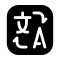
\includegraphics{./images/youtube/_Notes}

\end{column}

\begin{column}{0.001\textwidth}

~

\end{column}

\begin{column}{0.899\textwidth}

\begin{itemize}
\tightlist
\item
  \textbf{Weet je nog?} Czy pamiętasz?\\
\item
  \textbf{Ik weet het nog niet.} Nadal nie wiem.\\
\item
  \textbf{Ik zou graag naar Polen gaan.} Chciałbym pojechać do Polski.\\
\item
  \textbf{Zij gaan totaal voorbij aan het risico.} Całkowicie ignorują ryzyko.\\
\item
  \textbf{Ik heb nog niet gegeten.} Jeszcze nic nie jadłem.\\
\item
  \textbf{Mien is een vorm van Wilhelmina.} Mien jest formą Wilhelminy.
\end{itemize}

\end{column}

\vfill

\hypertarget{Het-is-een-nacht}{%
\section{\texorpdfstring{Het is een nacht, \emph{Guus Meeuwis}}{Het is een nacht, Guus Meeuwis}}\label{Het-is-een-nacht}}

\begin{column}{0.10\textwidth}

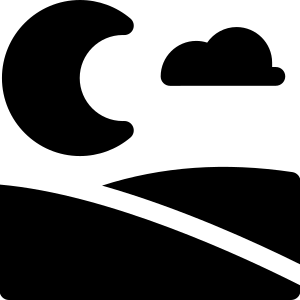
\includegraphics{./images/Het-is-een-nacht}

\end{column}

\begin{column}{0.04\textwidth}

~

\end{column}

\begin{column}{0.86\textwidth}

\textbf{Het is een nacht} \citep{Het-is-een-nacht} \href{https://youtu.be/BMqZIFVYUXw}{\includegraphics{./images/youtube/_Youtube}} \emph{Jest taka noc} powstała po romantycznym weekendzie, jaki spędził autor ze swoją dziewczyną Valérie Gregoire w Brugii.

\end{column}

\vfill

\begin{column}{0.48\textwidth}

Je vraagt of ik zin heb in een sigaret\\
Het is twee uur 's nachts\\
We liggen op bed\\
In een hotel in een stad\\
Waar niemand ons hoort\\
Waar niemand ons kent\\
En niemand ons stoort\\
Op de vloer ligt een lege fles wijn\\
En kledingstukken die van jou of mij kunnen zijn\\
Een schemering de radio zacht\\
En deze nacht heeft alles\\
Wat ik van een nacht verwacht

\end{column}

\begin{column}{0.04\textwidth}

~

\end{column}

\begin{column}{0.48\textwidth}

Pytasz, czy mam ochotę na papierosa\\
Jest druga w nocy\\
Jesteśmy w łóżku\\
W hotelu, w mieście\\
Gdzie nikt nas nie słyszy\\
Gdzie nikt nas nie zna\\
I nikt nam nie przeszkadza\\
Na podłodze leży pusta butelka po winie\\
I ubrania, które mogą być twoje lub moje\\
Półmrok, radio cicho gra\\
I ta noc ma wszystko\\
Czego oczekuję od nocy

\end{column}

\vfill

\begin{column}{0.48\textwidth}

\emph{Het is een nacht}\\
\emph{Die je normaal alleen in films ziet}\\
\emph{Het is een nacht}\\
\emph{Die wordt bezongen in het mooiste lied}\\
\emph{Het is een nacht}\\
\emph{Waarvan ik dacht dat ik hem nooit beleven zou}\\
\emph{Maar vannacht beleef ik hem met jou ohoh}

\end{column}

\begin{column}{0.04\textwidth}

~

\end{column}

\begin{column}{0.48\textwidth}

\emph{Jest taka noc}\\
\emph{Którą normalnie widzisz tylko w filmach}\\
\emph{Jest taka noc}\\
\emph{Którą wychwalają w najpiękniejszej piosence}\\
\emph{Jest taka noc}\\
\emph{Której nie spodziewałem się nigdy przeżyć}\\
\emph{Ale dziś w nocy przeżywam ją z tobą, Ooo}

\end{column}

\vfill

\begin{column}{0.48\textwidth}

Ik ben nog wakker en ik staar naar het plafond\\
En ik denk aan de dag lang geleden begon\\
Het zomaar er vandoor gaan met jou\\
Niet wetend waar de reis eindigen zou\\
Nu lig ik hier in een wildvreemde stad\\
En heb net de nacht van mijn leven gehad\\
Maar helaas er komt weer licht door de ramen\\
Hoewel voor ons de wereld\\
Vannacht heeft stil gestaan

\end{column}

\begin{column}{0.04\textwidth}

~

\end{column}

\begin{column}{0.48\textwidth}

Nadal nie śpię i wpatruję się w sufit\\
I myślę o tym dniu co zaczął się tak dawno\\
Tak po prostu przemija przy tobie\\
Nie wiedząc, gdzie zakończy się ta podróż\\
Teraz leżę tutaj w zupełnie obcym mieście\\
I właśnie miałem noc swojego życia\\
Ale niestety światło znów wpada przez okna\\
Ale co tam, świat dla nas\\
Zatrzymał się dziś w nocy

\end{column}

\vfill

\begin{column}{0.48\textwidth}

Maar een lied blijft slechts bij woorden\\
Een film is in scène gezet\\
Maar deze nacht met jou\\
Is levensecht

\end{column}

\begin{column}{0.04\textwidth}

~

\end{column}

\begin{column}{0.48\textwidth}

Ale piosenka to tylko słowa\\
Film został tylko zagrany\\
Ale dzisiejsza noc z tobą\\
Jest prawdziwa

\end{column}

\vfill

\begin{column}{0.48\textwidth}

En vannacht beleef ik hem met jou ohoh\\
En ik hou alleen nog maar van jou ohoh\\
En ik hou alleen nog maar van jou

\end{column}

\begin{column}{0.04\textwidth}

~

\end{column}

\begin{column}{0.48\textwidth}

I dziś przeżywam ją z tobą Ooo\ldots{}\\
I kocham tylko wyłącznie ciebie Ooo\ldots{}\\
I kocham tylko wyłącznie ciebie

\end{column}

\vfill

\begin{column}{0.10\textwidth}

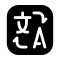
\includegraphics{./images/youtube/_Notes}

\end{column}

\begin{column}{0.001\textwidth}

~

\end{column}

\begin{column}{0.899\textwidth}

\begin{itemize}
\tightlist
\item
  \textbf{Je bent trouwens eigenlijk wel geweldig.} Nawiasem mówiąc, jesteś naprawdę świetny.\\
\item
  \textbf{Als ik niet Pools was, zou ik geen Pools kennen.} Gdybym nie był Polakiem, nie znałbym polskiego.\\
\item
  \textbf{Heb ik daarvoor een vergunning nodig?} Czy potrzebuję na to zezwolenie?\\
\item
  \textbf{Waar kan ik meer te weten komen over \ldots?} Gdzie mogę dowiedzieć się więcej o\ldots?\\
\item
  \textbf{Wanneer \ldots{}} Kiedy \ldots\ldots..?\\
\item
  \textbf{Ik heb zin in een borrel.} Mam ochotę na drinka.\\
\item
  \textbf{De lijn is bezet.} Linia jest zajęta.\\
\item
  \textbf{Als ik meer tijd had, zou ik op je wachten.} Gdybym miał/a więcej czasu, poczekałbym na ciebie.\\
\item
  \textbf{Je moeder kan echt lekker koken.} Twoja mama naprawdę potrafi dobrze gotować.\\
\item
  \textbf{Dat is veel, hè?} To dużo, co?\\
\item
  \textbf{Wanneer moet ik terugkomen?} Kiedy muszę wrócić?\\
\item
  \textbf{Zullen wij naar de duinen gaan?} Może pójdziemy na wydmy?
\end{itemize}

\end{column}

\vfill

\hypertarget{Ik-kan-het-niet-alleen}{%
\section{\texorpdfstring{Ik kan het niet alleen, \emph{De Dijk}}{Ik kan het niet alleen, De Dijk}}\label{Ik-kan-het-niet-alleen}}

\begin{column}{0.10\textwidth}

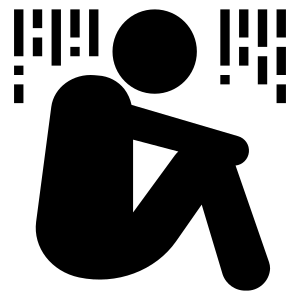
\includegraphics{./images/Ik-kan-het-niet-alleen}

\end{column}

\begin{column}{0.04\textwidth}

~

\end{column}

\begin{column}{0.86\textwidth}

\textbf{Ik kan het niet alleen} \citep{Ik-kan-het-niet-alleen} \href{https://youtu.be/ltSsojzp90M}{\includegraphics{./images/youtube/_Youtube}} \emph{Ja tak nie mogę sam} to jedna z najbardziej znanych piosenek De Dijk do dziś odtwarzana przez wiele stacji radiowych w Holandii..

\end{column}

\vfill

\begin{column}{0.48\textwidth}

Elke morgen\\
Elke middag\\
Elke avond\\
Iedere nacht

\end{column}

\begin{column}{0.04\textwidth}

~

\end{column}

\begin{column}{0.48\textwidth}

Każdego ranka\\
Każdego popołudnia\\
Każdego wieczoru\\
Każdej nocy

\end{column}

\vfill

\begin{column}{0.48\textwidth}

Stel dat ik er wel\\
Maar jij er niet was\\
Dan was morgen\\
Morgen waarschijnlijk weer zo'n dag

\end{column}

\begin{column}{0.04\textwidth}

~

\end{column}

\begin{column}{0.48\textwidth}

Co, jeśli tam byłem\\
A ty nie\\
Wtedy jutro\\
Jutro pewnie jest kolejny taki dzień

\end{column}

\vfill

\begin{column}{0.48\textwidth}

\emph{En ik kan het niet }\\
\emph{Ik kan er niet omheen }\\
\emph{Ik kan het niet }\\
\emph{Ik kan het niet alleen}

\end{column}

\begin{column}{0.04\textwidth}

~

\end{column}

\begin{column}{0.48\textwidth}

\emph{Ja tak nie mogę}\\
\emph{Nie mogę temu zaprzeczyć}\\
\emph{Ja tak nie mogę}\\
\emph{Ja tak nie mogę sam}

\end{column}

\vfill

\begin{column}{0.48\textwidth}

Natte ramen\\
Kale muren\\
Lege flessen\\
Lege flessen op de gang

\end{column}

\begin{column}{0.04\textwidth}

~

\end{column}

\begin{column}{0.48\textwidth}

Mokre okna\\
Gołe ściany\\
Puste butelki\\
Puste butelki na korytarzu

\end{column}

\vfill

\begin{column}{0.48\textwidth}

Lange tanden\\
Late uren\\
Weinig zon\\
Weinig zon en veel behang

\end{column}

\begin{column}{0.04\textwidth}

~

\end{column}

\begin{column}{0.48\textwidth}

Jedzenie bez smaku\\
Siedzenie do późna\\
Niewiele słońca\\
Niewiele słońca i pełno tapet

\end{column}

\vfill

\begin{column}{0.48\textwidth}

Ik heb het geprobeerd\\
Gedaan wat ik kan\\
Maar alles gaat verkeerd\\
Ik ben ook maar een man

\end{column}

\begin{column}{0.04\textwidth}

~

\end{column}

\begin{column}{0.48\textwidth}

Już próbowałem\\
Zrobiłem co mogłem\\
Ale wszystko idzie nie tak\\
Jestem tylko mężczyzną

\end{column}

\vfill

\begin{column}{0.48\textwidth}

En ik kan het niet alleen

\end{column}

\begin{column}{0.04\textwidth}

~

\end{column}

\begin{column}{0.48\textwidth}

Ja tak nie mogę sam

\end{column}

\vfill

\begin{column}{0.48\textwidth}

Elke morgen\\
's Middags\\
's Avonds\\
Maar vooral 's nachts

\end{column}

\begin{column}{0.04\textwidth}

~

\end{column}

\begin{column}{0.48\textwidth}

Każdego poranka\\
Po południu\\
Wieczorem\\
A zwłaszcza w nocy

\end{column}

\vfill

\begin{column}{0.48\textwidth}

Stel dat ik er wel\\
En jij er niet was\\
Dan was morgen\\
Morgen waarschijnlijk weer zo'n dag

\end{column}

\begin{column}{0.04\textwidth}

~

\end{column}

\begin{column}{0.48\textwidth}

Co, jeśli tam byłem\\
A ty nie\\
Wtedy jutro\\
Jutro pewnie jest kolejny taki dzień

\end{column}

\vfill

\begin{column}{0.10\textwidth}

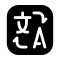
\includegraphics{./images/youtube/_Notes}

\end{column}

\begin{column}{0.001\textwidth}

~

\end{column}

\begin{column}{0.899\textwidth}

\begin{itemize}
\tightlist
\item
  \textbf{Weer zo'n dag uit het leven van Juf Nowak.} Kolejny dzień z życia panny Nowak.\\
\item
  \textbf{Hij eet met lange tanden.} On je niechętnie.\\
\item
  \textbf{Beter laat dan nooit.} Lepiej późno niż wcale.\\
\item
  \textbf{We kunnen er niet omheen dat \ldots{}} Nie możemy omijać faktu, że \ldots{}\\
\item
  \textbf{We nemen Agata ook maar mee.} Zabieramy również Agatę ze sobą.\\
\item
  \textbf{Ik ben ook maar een mens.} Jestem tylko człowiekiem.
\end{itemize}

\end{column}

\vfill

\hypertarget{Ik-voel-me-zo-verdomd-alleen}{%
\section{\texorpdfstring{Ik Voel Me Zo Verdomd Alleen, \emph{Danny De Munk}}{Ik Voel Me Zo Verdomd Alleen, Danny De Munk}}\label{Ik-voel-me-zo-verdomd-alleen}}

\begin{column}{0.10\textwidth}

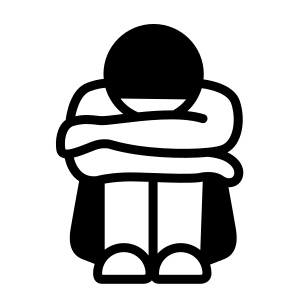
\includegraphics{./images/Ik-voel-me-zo-verdomd-alleen}

\end{column}

\begin{column}{0.04\textwidth}

~

\end{column}

\begin{column}{0.86\textwidth}

\textbf{Ik Voel Me Zo Verdomd Alleen} \citep{Ik-voel-me-zo-verdomd-alleen} \href{https://youtu.be/G-JcK8MbWFw}{\includegraphics{./images/youtube/_Youtube}} \emph{Czuję się tak cholernie samotny} pochodzi z filmu `Ciske de Rat' opartego na książkach Piet Bakkera. Danny De Munk zagrał w nim i wykonał tytułową piosenką.

\end{column}

\vfill

\begin{column}{0.48\textwidth}

Krijg toch allemaal de klere\\
Val voor mijn part allemaal dood\\
Ik heb geen zin om braaf te leren\\
Ik eindig toch wel in de goot\\
Kinderen willen niet met me spelen\\
Noemen me Rat en wijzen me na\\
De enige die me wat kan schelen\\
Die is er nooit, dat is m'n pa

\end{column}

\begin{column}{0.04\textwidth}

~

\end{column}

\begin{column}{0.48\textwidth}

Oby was wszystkich wzięła cholera\\
Dla mnie wszyscy padnijcie trupem\\
Nie mam zamiaru grzecznie się uczyć\\
I tak skończę w rynsztoku\\
Dzieci nie chcą się ze mną bawić\\
Nazywają mnie Szczurem i pokazują palcem\\
Jedyny, kto dla mnie cokolwiek znaczy\\
A którego nigdy nie ma, to jest mój tata

\end{column}

\vfill

\begin{column}{0.48\textwidth}

M'n moeder kan me niet verdragen\\
Nooit doe ik iets voor haar goed\\
Om liefde hoef ik ook al niet te vragen\\
Schelden is alles wat ze doet\\
Geen wonder dat m'n pa is gaan varen\\
Ik mocht niet mee, ik ben te klein\\
Ik moet 't in m'n eentje klaren\\
Tot 'ie ooit weer terug zal zijn

\end{column}

\begin{column}{0.04\textwidth}

~

\end{column}

\begin{column}{0.48\textwidth}

Moja matka nie może mnie znieść\\
Dla niej niczego nigdy nie robię dobrze\\
O miłość nawet nie ma co pytać\\
Wszystko co ona potrafi, to mnie zwymyślać\\
Nic dziwnego, że mój tata wypłynął w morze\\
Nie mogłem razem z nim, jestem za mały\\
Muszę samemu to jakoś wyklarować\\
Zanim on kiedyś tu będzie z powrotem

\end{column}

\vfill

\begin{column}{0.48\textwidth}

\emph{Had ik maar iemand om van te houden}\\
\emph{Twee zachte armen om me heen}\\
\emph{Die mij altijd beschermen zouden}\\
\emph{Ik voel me zo verdomd alleen}

\end{column}

\begin{column}{0.04\textwidth}

~

\end{column}

\begin{column}{0.48\textwidth}

\emph{Gdybym miał tylko kogoś do kochania}\\
\emph{Wokół siebie dwa miękkie ramiona}\\
\emph{Które będą zawsze mnie chronić}\\
\emph{Czuję się tak cholernie samotny}

\end{column}

\vfill

\begin{column}{0.48\textwidth}

Misschien als vaders schip er is\\
Als 'ie weer terug is van de zee\\
Zegt 'ie nog eens luister Cis\\
Waarom ga je niet met me mee\\
Ik ben toch ook nog maar een kind\\
Kan 't niet helemaal alleen\\
Misschien dat ik ooit het geluk nog vind\\
Maar hoe, dat is een groot probleem

\end{column}

\begin{column}{0.04\textwidth}

~

\end{column}

\begin{column}{0.48\textwidth}

Może, jak statek ojca tutaj będzie\\
Jak on się z morza wróci\\
Powie raz jeszcze, słuchaj Cis\\
Dlaczego nie wybierzesz się ze mną\\
Ja przecież jeszcze jestem dzieckiem\\
Nie mogę tego zrobić zupełnie sam\\
Możliwe, że kiedyś jeszcze znajdę szczęście\\
Ale jak, to już jest duży problem

\end{column}

\vfill

\begin{column}{0.10\textwidth}

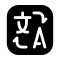
\includegraphics{./images/youtube/_Notes}

\end{column}

\begin{column}{0.001\textwidth}

~

\end{column}

\begin{column}{0.899\textwidth}

\begin{itemize}
\tightlist
\item
  \textbf{Kolere en klere zijn hetzelfde.} Cholera i cholercia to to samo.\\
\item
  \textbf{Voor mijn part \ldots{}} Jeżeli chodzi o mnie \ldots{}\\
\item
  \textbf{Ik mag dood vallen als het niet waar is.} Niech padnę trupem, jeśli to nieprawda.\\
\item
  \textbf{Het kan me niets schelen.} Jest mi wszystko jedno.\\
\item
  \textbf{Tomek kwam hier in zijn eentje.} Tomek przyszedł tu sam.\\
\item
  \textbf{Ik heb mijn werk geklaard.} Wykonałem swoją pracę.\\
\item
  \textbf{Zou ik wachten tot ze weer komt?} Czy powinienem czekać na jej powrót?\\
\item
  \textbf{Hij was helemaal alleen in het huis.} On był zupełnie sam w domu.\\
\item
  \textbf{Ik hoef niet af te vallen.} Ja nie muszę się odchudzać.\\
\item
  \textbf{Als ik vragen mag \ldots{}} Jeżeli wolno spytać \ldots{}\\
\item
  \textbf{Ik bel je morgen, als ik weer terug ben.} Zadzwonię do ciebie jutro po powrocie.\\
\item
  \textbf{Ik kan het niet alleen.} Nie mogę tego zrobić sam. \ref{Ik-kan-het-niet-alleen}
\end{itemize}

\end{column}

\vfill

\hypertarget{La-vie-est-belle}{%
\section{\texorpdfstring{La vie est belle, \emph{Diggy Dex ft. DJ Vali}}{La vie est belle, Diggy Dex ft. DJ Vali}}\label{La-vie-est-belle}}

\begin{column}{0.10\textwidth}

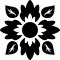
\includegraphics{./images/La-vie-est-belle}

\end{column}

\begin{column}{0.04\textwidth}

~

\end{column}

\begin{column}{0.86\textwidth}

\textbf{La vie est belle} \citep{La-vie-est-belle} \href{https://youtu.be/DLTq19bhO28}{\includegraphics{./images/youtube/_Youtube}} \emph{Życie jest piękne} \ldots{} . Koen Jansen (Diggy Dex) napisał również tekst do piosenki \ref{Leef}.

\end{column}

\vfill

\begin{column}{0.48\textwidth}

Geld laat de wereld draaien\\
Liefde laat de wereld zien\\
't Was het eerste wat ik opschreef vanochtend toen ik opstond\\
't Was blijkbaar wat er opkomt

\end{column}

\begin{column}{0.04\textwidth}

~

\end{column}

\begin{column}{0.48\textwidth}

Pieniądz pozwala światu się kręcić\\
Miłość pozwala światu widzieć\\
To była pierwsza rzecz, którą zapisałem dziś rano, kiedy wstałem\\
To było jasne, co się okazało

\end{column}

\vfill

\begin{column}{0.48\textwidth}

'k Kleed me aan en m'n zoon ook\\
Rij naar school, rij terug, pak de krant, sla hem open\\
En m'n ogen dwalen door een tekst\\
Zoveel drama op een afstand het blijft toch iets geks

\end{column}

\begin{column}{0.04\textwidth}

~

\end{column}

\begin{column}{0.48\textwidth}

Ubieram siebie i swojego syna też\\
Jadę do szkoły, jadę z powrotem, biorę gazetę, otwieram ją\\
I moje oczy wędrują po tekście\\
Tyle dramatu na odległość pozostaje jednak czymś szalonym

\end{column}

\vfill

\begin{column}{0.48\textwidth}

Pak m'n tas, loop naar buiten,\\
Krijg plots een berichtje van een vriend met luister deze moet je even horen\\
't Is vreemd hoe het werkt\\
Hoe iemand z'n verdriet ertoe kan leiden dat een prachtig lied wordt geboren

\end{column}

\begin{column}{0.04\textwidth}

~

\end{column}

\begin{column}{0.48\textwidth}

Chwytam moją torbę, wychodzę na zewnątrz,\\
Nagle dostaję wiadomość od znajomego ze słyszysz musisz tego posłuchać\\
To dziwne, jak to działa\\
Jak czyjaś żałoba może doprowadzić do tego, że przychodzi na świat piękna piosenka

\end{column}

\vfill

\begin{column}{0.48\textwidth}

Loop verder naar de trein, m'n ogen vallen op een vrouw\\
Niet helemaal honderd, althans volgens onze regels\\
Iedereen die blijft naar haar kijken, terwijl ik zie dat ze danst in de regen\\
We doen het allemaal met wat je krijgt hier vooral het leven

\end{column}

\begin{column}{0.04\textwidth}

~

\end{column}

\begin{column}{0.48\textwidth}

Idę dalej na pociąg, moje oczy padają na kobietę\\
Niecałe sto, przynajmniej według naszych zasad\\
Każdy, kto został na nią patrzy, podczas gdy ja widzę, że ona tańczy w deszczu\\
Wszyscy to robimy z tym co tu dostajemy, zwłaszcza życiem

\end{column}

\vfill

\begin{column}{0.48\textwidth}

\emph{\textbf{La vie est belle} Het leven is prachtig ×3}\\
\emph{\textbf{Je n'y comprends rien} Ik begrijp er niets van}\\
\emph{\textbf{Je vais rire jusqu'à la fin} Ik zal lachen tot het einde}\\
\emph{\textbf{La vie est belle} Het leven is prachtig ×2}

\end{column}

\begin{column}{0.04\textwidth}

~

\end{column}

\begin{column}{0.48\textwidth}

\emph{Życie jest piękne ×3}\\
\emph{Nic z tego nie rozumiem}\\
\emph{Będę śmiać się do końca}\\
\emph{Życie jest piękne ×2}

\end{column}

\vfill

\begin{column}{0.48\textwidth}

Stap uit in de stad en begin te lopen\\
Langs nieuwe straten waar ik vroeger van gedroomd heb\\
Uit verlangens van een nooit geleefd leven\\
Koptelefoon op en de radio op play

\end{column}

\begin{column}{0.04\textwidth}

~

\end{column}

\begin{column}{0.48\textwidth}

Wysiadam na mieście i zaczynam iść\\
Wzdłuż nowych ulic, o których kiedyś marzyłem\\
Z pragnień nigdy nie przeżywanego życia\\
Słuchawki na uszach i radio na play

\end{column}

\vfill

\begin{column}{0.48\textwidth}

'k Hoor een man terug van weggeweest zeggen\\
't Ging even niet zo best, laat me rustig uitleggen\\
'k Heb net m'n vrouw verloren\\
Terwijl hij haar beschrijft voel ik de glimlach verborgen in zijn stem

\end{column}

\begin{column}{0.04\textwidth}

~

\end{column}

\begin{column}{0.48\textwidth}

Słyszę mężczyznę z powrotem w grze mówiącego\\
Przez jakiś czas nie szło tak dobrze, pozwól na spokojnie wyjaśnię\\
Właśnie straciłem żonę\\
Kiedy ją opisuje, czuję uśmiech ukryty w jego głosie

\end{column}

\vfill

\begin{column}{0.48\textwidth}

En ik denk nog eens terug aan al die eindeloze nachten\\
Aan m'n vrienden, m'n geliefden en ook soms de donkerste gedachten\\
Waar ik was al die tijd weet ik niet\\
Misschien ergens op een plek waar ik veel te veel verwachtte

\end{column}

\begin{column}{0.04\textwidth}

~

\end{column}

\begin{column}{0.48\textwidth}

I myślę z powrotem o tych wszystkich niekończących się nocach\\
O moich przyjaciołach, moich ukochanych i czasami najciemniejszych myślach\\
Gdzie ja byłem przez cały ten czas nie wiem\\
Może w miejscu, gdzie dużo za dużo oczekiwałem

\end{column}

\vfill

\begin{column}{0.48\textwidth}

Bestel wat te drinken en schrijf wat op, betaal de ober, loop weg\\
En vervolg m'n tocht richting een brug waar een man staat te gebaren\\
'k Denk, ach 't zal wel, ik laat 'm\\
Kijk nog een keer om, het is een vriend, hij zwaait

\end{column}

\begin{column}{0.04\textwidth}

~

\end{column}

\begin{column}{0.48\textwidth}

Zamawiam coś do picia i coś notuję, płacę kelnerowi, uciekam\\
I kontynuuję moją podróż w kierunku mostu, na którym gestykuluje mężczyzna\\
Myślę, a co tam, zostawiam go\\
Spoglądam jeszcze raz, to przyjaciel, on macha

\end{column}

\vfill

\begin{column}{0.10\textwidth}

\includegraphics{./images/youtube/_Notes}

\end{column}

\begin{column}{0.001\textwidth}

~

\end{column}

\begin{column}{0.899\textwidth}

\begin{itemize}
\tightlist
\item
  \textbf{De kinderen horen alles, maar luisteren zelden.} Dzieci słyszą wszystko, ale rzadko słuchają.\\
\item
  \textbf{Daar kun je geen nee tegen zeggen.} Nie możesz odmówić.\\
\item
  \textbf{Je kijkt wel, maar je ziet niks.} Patrzysz, ale nic nie widzisz.\\
\item
  \textbf{Wil je weglopen van huis?} Chcesz uciec z domu?\\
\item
  \textbf{Ik ben terug van weggeweest.} Wróciłem do gry.\\
\item
  \textbf{We zijn ergens op een godverlaten plek.} Jesteśmy w miejscu zapomnianym przez boga.
\end{itemize}

\end{column}

\vfill

\hypertarget{Leef}{%
\section{\texorpdfstring{Leef, \emph{André Hazes jr.}}{Leef, André Hazes jr.}}\label{Leef}}

\begin{column}{0.10\textwidth}

\includegraphics{./images/Leef}

\end{column}

\begin{column}{0.04\textwidth}

~

\end{column}

\begin{column}{0.86\textwidth}

\textbf{Leef} \citep{Leef} \href{https://youtu.be/2H0yWKdZM8g}{\includegraphics{./images/youtube/_Youtube}} \emph{Żyj} to piosenka o życiu i umieraniu. Rozpoczyna się w scenerii podobnej do tej z piosenki \ref{Een-beetje-verliefd} wykonanej przez ojca André Hazes.

\end{column}

\vfill

\begin{column}{0.48\textwidth}

Op een vrijdag in de kroeg ergens in Amsterdam\\
Zat aan de bar met een glas een oude wijze man\\
Hij zei dat die nog maar een paar dagen had\\
Dus pak het leven, pak alles en ga er mee op pad

\end{column}

\begin{column}{0.04\textwidth}

~

\end{column}

\begin{column}{0.48\textwidth}

W piątek w pubie w Amsterdamie siedział\\
Stary mądry człowiek ze szklanką przy barze\\
Powiedział, że zostało mu jeszcze tylko kilka dni\\
Więc chwytaj życie, weź wszystko i ruszaj ze mną

\end{column}

\vfill

\begin{column}{0.48\textwidth}

\emph{En hij zei: '\,'Leef, alsof het je laatste dag is}\\
\emph{Leef, alsof de morgen niet bestaat}\\
\emph{Leef, alsof het nooit echt af is}\\
\emph{En leef, pak alles wat je kan'\,'}

\end{column}

\begin{column}{0.04\textwidth}

~

\end{column}

\begin{column}{0.48\textwidth}

\emph{I rzekł: '\,'Żyj, jakby to był twój ostatni dzień}\\
\emph{Żyj, jakby nie miało być jutra}\\
\emph{Żyj, jakby to nie był koniec do końca}\\
\emph{I żyj, łap wszystko'\,'}

\end{column}

\vfill

\begin{column}{0.48\textwidth}

\emph{En ga, a, a, a}\\
\emph{A, a, a, a}\\
\emph{A, a, a, a}\\
\emph{Pak alles wat je kan}

\end{column}

\begin{column}{0.04\textwidth}

~

\end{column}

\begin{column}{0.48\textwidth}

\emph{I leć, a, a, a}\\
\emph{A, a, a, a}\\
\emph{A, a, a, a}\\
\emph{Łap wszystko, co możesz}

\end{column}

\vfill

\begin{column}{0.48\textwidth}

\emph{En ga, a, a, a}\\
\emph{A, a, a, a}\\
\emph{Ga}\\
\emph{Pak alles wat je kan}

\end{column}

\begin{column}{0.04\textwidth}

~

\end{column}

\begin{column}{0.48\textwidth}

\emph{I leć, a, a, a}\\
\emph{A, a, a, a}\\
\emph{Leć}\\
\emph{Łap wszystko, co możesz}

\end{column}

\vfill

\begin{column}{0.48\textwidth}

Hij vertelde dat 'ie zich had gewerkt in het zweet\\
Geld verdiend als water maar nooit echt had geleefd\\
Z'n vrouw was bij hem weg, voor een ander ingeruild\\
Af en toe gelachen maar veel te veel gehuild

\end{column}

\begin{column}{0.04\textwidth}

~

\end{column}

\begin{column}{0.48\textwidth}

Opowiedział, jak się w życiu napocił przy robocie\\
Pieniądze spływały lekko ale nigdy nie żył naprawdę\\
Żona go opuściła zamieniła sobie na innego\\
Zbyt mało śmiał się a zbyt dużo się napłakał

\end{column}

\vfill

\begin{column}{0.10\textwidth}

\includegraphics{./images/youtube/_Notes}

\end{column}

\begin{column}{0.001\textwidth}

~

\end{column}

\begin{column}{0.899\textwidth}

\begin{itemize}
\tightlist
\item
  \textbf{Hij is zo vlug als water.} On chwyta w biegu.\\
\item
  \textbf{Ik wilde net op pad gaan.} Właśnie miałem wyruszyć w drogę.\\
\item
  \textbf{Gele gans zelf.} Zażółć gęślą jaźń.
\end{itemize}

\end{column}

\vfill

\hypertarget{Liefs-uit-Londen}{%
\section{\texorpdfstring{Liefs uit Londen, \emph{BLØF}}{Liefs uit Londen, BLØF}}\label{Liefs-uit-Londen}}

\begin{column}{0.10\textwidth}

\includegraphics{./images/Liefs-uit-Londen}

\end{column}

\begin{column}{0.04\textwidth}

~

\end{column}

\begin{column}{0.86\textwidth}

\textbf{Liefs uit Londen} \citep{Liefs-uit-Londen} \href{https://youtu.be/aM5JU0juOSs}{\includegraphics{./images/youtube/_Youtube}} \emph{Kocham z Londynu} to pierwszy z hitów grupy BLØF, którego tekst był zainspirowany grą planszową `Podróż dookoła świata'.

\end{column}

\vfill

\begin{column}{0.48\textwidth}

Van de wereld weet ik niets, niets dan wat ik hoor en zie, niets dan wat ik lees\\
Ik ken geen andere landen, zelfs al ben ik er geweest

\end{column}

\begin{column}{0.04\textwidth}

~

\end{column}

\begin{column}{0.48\textwidth}

O świecie nie wiem nic, nic oprócz tego co słyszę i widzę, nic oprócz tego co czytam\\
Nie znam innych krajów, nawet jeśli tam byłem

\end{column}

\vfill

\begin{column}{0.48\textwidth}

Grote steden ken ik niet behalve uit de boeken, behalve van tv\\
Ik ken geen andere stad dan de stad waarin ik leef

\end{column}

\begin{column}{0.04\textwidth}

~

\end{column}

\begin{column}{0.48\textwidth}

Dużych miast nie znam tyle co z książek, tyle co z telewizji\\
Nie znam innego miasta niż to, w którym żyję

\end{column}

\vfill

\begin{column}{0.48\textwidth}

\emph{Zij stuurt me kaarten uit Madrid en uit Moskou komt een brief met de prachtigste verhalen}\\
\emph{Oh God, wat is ze lief}\\
\emph{Gisteren uit Lissabon `'ik mis je'' en een zoen}

\end{column}

\begin{column}{0.04\textwidth}

~

\end{column}

\begin{column}{0.48\textwidth}

\emph{Ona wysyła mi kartki z Madrytu, a z Moskwy przyszedł list z najpiękniejszymi opowieściami}\\
\emph{Mój Boże, jaka ona jest kochana}\\
\emph{Wczoraj z Lizbony `'tęsknię za tobą'' i całus }

\end{column}

\vfill

\begin{column}{0.48\textwidth}

\emph{Vandaag uit Praag een kattebel, want er is zoveel te doen}\\
\emph{En morgen, als de postbode mijn huis weer heeft gevonden dan stort ze mijn hart vol met al het liefs uit Londen}

\end{column}

\begin{column}{0.04\textwidth}

~

\end{column}

\begin{column}{0.48\textwidth}

\emph{Dzisiaj z Pragi jakiś gryzmoł, bo tam jest tyle do roboty }\\
\emph{A jutro, gdy tylko listonosz znajdzie mój dom, ona napełni moje serce do pełna tymi wszystkimi kocham z Londynu }

\end{column}

\vfill

\begin{column}{0.48\textwidth}

Van de wereld weet ik niets, niets dan wat ik hoor en zie, niets dan wat ik voel\\
Ik leef van dag tot dag, zonder vrees en zonder doel

\end{column}

\begin{column}{0.04\textwidth}

~

\end{column}

\begin{column}{0.48\textwidth}

O świecie nie wiem nic, nic oprócz tego co słyszę i widzę, nic oprócz tego co czuję\\
Żyję z dnia na dzień, bez obaw i bez celu

\end{column}

\vfill

\begin{column}{0.48\textwidth}

Verre landen ken ik niet behalve uit mijn atlas, die droom ik elke nacht\\
Maar ik droom alleen de landen waar ze ooit aan me dacht

\end{column}

\begin{column}{0.04\textwidth}

~

\end{column}

\begin{column}{0.48\textwidth}

Odległych krajów nie znam tyle co z mojego atlasu, który śni mi się co noc\\
Ale śnią mi się tylko te kraje, w których ona kiedyś o mnie myślała

\end{column}

\vfill

\begin{column}{0.48\textwidth}

Als een mooi en groot geloof aan de muur van mijn gedachten hangt een wereldkaart te wachten tot ze terugkomt\\
Met haar reizen in mijn hoofd steek ik vlaggen in de aarde, dezelfde kleur, dezelfde waarde

\end{column}

\begin{column}{0.04\textwidth}

~

\end{column}

\begin{column}{0.48\textwidth}

Jak piękna i wielka wiara, na ścianie moich myśli wisi mapa świata czekając aż ona wróci\\
Wraz z jej podróżami, w myślach wtykam w ziemię flagi, ten sam kolor, to samo znaczenie

\end{column}

\vfill

\begin{column}{0.48\textwidth}

Maar \ldots{}

\end{column}

\begin{column}{0.04\textwidth}

~

\end{column}

\begin{column}{0.48\textwidth}

Lecz \ldots{}

\end{column}

\vfill

\begin{column}{0.10\textwidth}

\includegraphics{./images/youtube/_Notes}

\end{column}

\begin{column}{0.001\textwidth}

~

\end{column}

\begin{column}{0.899\textwidth}

\begin{itemize}
\tightlist
\item
  \textbf{Ik weet van niks.} Nic nie wiem.\\
\item
  \textbf{Ik ga, zelfs al regent het.} Idę, chociaż już pada deszcz.\\
\item
  \textbf{Behalve hij, kwam niemand naar het feestje.} Poza nim, nikt nie przyszedł na przyjęcie.\\
\item
  \textbf{Ik ken geen van drieën.} Nie znam nikogo z tej trójki.\\
\item
  \textbf{Ik ken u niet.} Nie znam Pan-i/a.\\
\item
  \textbf{Is zijn verhaal waar?} Czy jego historia jest prawdziwa?\\
\item
  \textbf{Ik vrees van niet.} Obawiam się, że nie.\\
\item
  \textbf{Wat ben je mooi.} Jaka jesteś piękna.\\
\item
  \textbf{Ik wil je zoenen.} Chcę cię pocałować.\\
\item
  \textbf{U mag nu de bruid kussen.} Możesz teraz pocałować pannę młodą.\\
\item
  \textbf{Als je me laat spreken, dan kan ik alles uitleggen.} Jak pozwolisz mi mówić, wtedy ja mogę wszystko wyjaśnić.
\end{itemize}

\end{column}

\vfill

\hypertarget{Mag-ik-dan-bij-jou}{%
\section{\texorpdfstring{Mag ik dan bij jou, \emph{Claudia de Breij}}{Mag ik dan bij jou, Claudia de Breij}}\label{Mag-ik-dan-bij-jou}}

\begin{column}{0.10\textwidth}

\includegraphics{./images/Mag-ik-dan-bij-jou}

\end{column}

\begin{column}{0.04\textwidth}

~

\end{column}

\begin{column}{0.86\textwidth}

\textbf{Mag ik dan bij jou} \citep{Mag-ik-dan-bij-jou} \href{https://youtu.be/o5uvsEs79hM}{\includegraphics{./images/youtube/_Youtube}} \emph{Czy będę mogła przy tobie?} to wyznanie miłosne wypełnione przypuszczeniami.

\end{column}

\vfill

\begin{column}{0.48\textwidth}

Als de oorlog komt en als ik dan moet schuilen\\
Mag ik dan bij jou?\\
Als er een clubje komt waar ik niet bij wil horen\\
Mag ik dan bij jou?

\end{column}

\begin{column}{0.04\textwidth}

~

\end{column}

\begin{column}{0.48\textwidth}

Jeżeli wybuchnie wojna i jeżeli wtedy będę musiała się skryć\\
To, czy będę mogła przy tobie?\\
Jeżeli powstanie klub, w którym nie chcę być\\
To, czy będę mogła przy tobie?

\end{column}

\vfill

\begin{column}{0.48\textwidth}

Als er een regel komt waar ik niet aan voldoen kan\\
Mag ik dan bij jou?\\
En als ik iets moet zijn wat ik nooit geweest ben\\
Mag ik dan bij jou?

\end{column}

\begin{column}{0.04\textwidth}

~

\end{column}

\begin{column}{0.48\textwidth}

Jeżeli wejdzie reguła, której nie mogę spełnić\\
To, czy będę mogła przy tobie?\\
Jeżeli będę musiała stać się kimś, kim nigdy nie byłam\\
To, czy będę mogła przy tobie?

\end{column}

\vfill

\begin{column}{0.48\textwidth}

\emph{Mag ik dan bij jou schuilen als het nergens anders kan?}\\
\emph{En als ik moet huilen droog jij m'n tranen dan?}\\
\emph{Want als ik bij jou mag, mag jij altijd bij mij}\\
\emph{Kom wanneer je wilt ik hou een kamer voor je vrij}

\end{column}

\begin{column}{0.04\textwidth}

~

\end{column}

\begin{column}{0.48\textwidth}

\emph{Czy będę mogła przy tobie się skryć, gdy nie będzie gdzie indziej?}\\
\emph{I jeżeli będę musiała zapłakać, to czy wysuszysz me łzy?}\\
\emph{Bo jeżeli ja mogę przy tobie, to ty zawsze możesz przy mnie}\\
\emph{Przyjdź kiedy tylko chcesz, mam dla ciebie wolny pokój}

\end{column}

\vfill

\begin{column}{0.48\textwidth}

Als het onweer komt en als ik dan bang ben\\
Mag ik dan bij jou?\\
Als de avond valt en 't is mij te donker\\
Mag ik dan bij jou?

\end{column}

\begin{column}{0.04\textwidth}

~

\end{column}

\begin{column}{0.48\textwidth}

Jeżeli nadejdzie burza i jeżeli wtedy będę się bać\\
To, czy będę mogła przy tobie?\\
Jeżeli zapadnie wieczór i dla mnie stanie się za ciemno\\
To, czy będę mogła przy tobie?

\end{column}

\vfill

\begin{column}{0.48\textwidth}

Als de lente komt en als ik dan verliefd ben\\
Mag ik dan bij jou?\\
Als de liefde komt en ik weet het zeker\\
Mag ik dan bij jou?

\end{column}

\begin{column}{0.04\textwidth}

~

\end{column}

\begin{column}{0.48\textwidth}

Jeżeli przyjdzie wiosna i jeżeli wtedy się zakocham\\
To, czy będę mogła przy tobie?\\
Jeżeli przyjdzie miłość i jeżeli będę tego pewna\\
To, czy będę mogła przy tobie?

\end{column}

\vfill

\begin{column}{0.48\textwidth}

Als het einde komt en als ik dan bang ben\\
Mag ik dan bij jou?\\
Als het einde komt en als ik dan alleen ben\\
Mag ik dan bij jou?

\end{column}

\begin{column}{0.04\textwidth}

~

\end{column}

\begin{column}{0.48\textwidth}

Jeżeli nadejdzie koniec i jeżeli wtedy będę się bać\\
To, czy będę mogła przy tobie?\\
Jeżeli nadejdzie koniec i jeżeli wtedy zostanę sama\\
To, czy będę mogła przy tobie?

\end{column}

\vfill

\begin{column}{0.10\textwidth}

\includegraphics{./images/youtube/_Notes}

\end{column}

\begin{column}{0.001\textwidth}

~

\end{column}

\begin{column}{0.899\textwidth}

\begin{itemize}
\tightlist
\item
  \textbf{Mogen we bij jou overnachten?} Czy możemy u ciebie przenocować?\\
\item
  \textbf{De spullen moeten wel aan één regel voldoen.} Przedmioty muszą być zgodne z jedną zasadą.\\
\item
  \textbf{Dat is jouw thuis, daar en nergens anders.} To jest twój dom, tam i nigdzie indziej.\\
\item
  \textbf{Als je niets te zeggen hebt, zeg dan niets.} Jeśli nie masz nic do powiedzenia, nie mów nic.
\end{itemize}

\end{column}

\vfill

\hypertarget{Nacht}{%
\section{\texorpdfstring{Nacht, \emph{Guus Meeuwis \& Kraantje Pappie}}{Nacht, Guus Meeuwis \& Kraantje Pappie}}\label{Nacht}}

\begin{column}{0.10\textwidth}

\includegraphics{./images/Nacht}

\end{column}

\begin{column}{0.04\textwidth}

~

\end{column}

\begin{column}{0.86\textwidth}

\textbf{Nacht} \citep{Nacht} \href{https://youtu.be/MxkdVogPeF0}{\includegraphics{./images/youtube/_Youtube}} \emph{Noc} to nowa wersja 25-letniego utworu ``Het is een nacht'' \ref{Het-is-een-nacht}.

\end{column}

\vfill

\begin{column}{0.48\textwidth}

\emph{Het is een nacht}\\
\emph{Die je normaal alleen in films ziet}\\
\emph{Het is een nacht}\\
\emph{Die wordt bezongen in het mooiste lied}\\
\emph{Het is een nacht}\\
\emph{Waarvan ik dacht dat ik 'm nooit beleven zou}\\
\emph{Maar vannacht beleef ik 'm met jou, oh}

\end{column}

\begin{column}{0.04\textwidth}

~

\end{column}

\begin{column}{0.48\textwidth}

\emph{Jest taka noc}\\
\emph{Którą normalnie widzisz tylko w filmach}\\
\emph{Jest taka noc}\\
\emph{Którą wychwalają w najpiękniejszej piosence}\\
\emph{Jest taka noc}\\
\emph{Której nie spodziewałem się nigdy przeżyć}\\
\emph{Ale dziś w nocy przeżywam ją z tobą, Ooo}

\end{column}

\vfill

\begin{column}{0.48\textwidth}

Op de grond ligt een Châteauneuf-du-Pape\\
De radio zacht, rond middernacht\\
Ik hoor Suus en Freek, een Blauwe Dag\\
En ik kijk hoe je slaapt, ik hou je vast\\
Want ik weet dat het niet lang meer duurt voor jij gaat\\
Ik snap dat jij me niet te dichtbij laat\\
En je weer vrijmaakt, en je op tijd staat\\
Je twijfelt aan of ik echt meen wat ik heb gezegd\\
En of ik nog steeds wel de echte ben\\
En of ik niet ren naar 050 en je niet meer ken als een slechte vent\\
Maar vannacht is dat allemaal niet de case\\
Voor nu is het nog nooit zo mooi geweest\\
Jij en ik, the world can wait\\
En ben ik voor eerst opeens compleet

\end{column}

\begin{column}{0.04\textwidth}

~

\end{column}

\begin{column}{0.48\textwidth}

Na ziemi leży Châteauneuf-du-Pape\\
Radio cicho gra, jest koło północy\\
Słyszę Suus i Freek, Blauwe Dag\\
Patrzę jak śpisz, przytulam cię mocno\\
Bo wiem, że to nie potrwa już długo zanim wyjdziesz\\
Rozumiem, że nie pozwolisz mi się zbliżyć\\
I uwolnisz się ponownie i wstaniesz na czas\\
Wątpisz, czy naprawdę myślę co powiedziałem\\
I czy nadal jestem prawdziwy\\
I czy nie biegnę na 50 i już cię nie znam jak jakiś zły facet\\
Ale dziś w nocy to w ogóle nie o to chodzi\\
Jeszcze nigdy nie było tak pięknie\\
Ty i ja, świat może poczekać\\
Nagle po raz pierwszy jestem spełniony

\end{column}

\vfill

\begin{column}{0.48\textwidth}

\emph{Als het kon, zou ik steeds met je zijn}\\
\emph{En als je wennen moet, begrijp ik baby, neem je de tijd}\\
\emph{Hier leven we voor, plus cash en baguettes}\\
\emph{En deze nacht heeft alles wat ik zocht op deze plek}

\end{column}

\begin{column}{0.04\textwidth}

~

\end{column}

\begin{column}{0.48\textwidth}

\emph{Byłbym z tobą zawsze, gdybym tylko mógł}\\
\emph{Ale jeśli musisz się zastanowić, rozumiem to baby, nie spiesz się}\\
\emph{Po to żyjemy, plus kasa i bagietki}\\
\emph{I ta noc ma wszystko, czego szukałem w tym miejscu}

\end{column}

\vfill

\begin{column}{0.48\textwidth}

Hey schat, ik zou m'n kleine teen geven voor nog één nacht\\
Het is natuurlijk geen wonder dat ik je\\
Donderdag al bijzonder zag in het dons gepakt heb\\
En onze nacht werd d'r een als\\
Die van Leo en Kate was\\
We on top of the world, ben volledig gebrainwashed\\
But I like it, yeah, jij showt wat life is\\
En ja, je life is er een als Kylie's\\
Maar net iets ronder en iets gezonder\\
Dat is precies hoe mijn vibe is, yeah\\
Jij bent de nicest\\
Bel de bellboy, bestel champagne\\
Fuck the prices, je rolt met Crane

\end{column}

\begin{column}{0.04\textwidth}

~

\end{column}

\begin{column}{0.48\textwidth}

Hej kochanie, oddałbym mój mały palec u nogi za jeszcze jedną noc\\
Nic dziwnego, że po tym jak cię w czwartek,\\
Choć szczególny zobaczyłem, zabrałem cię do łóżka\\
A nasza noc stała się taką,\\
Jaką mieli Leo i Kate\\
Jesteśmy na szczycie świata, mam kompletnie wyprany mózg\\
Ale lubię to, tak, pokazujesz, czym jest życie\\
I tak, twoje życie przypomina życie Kylie\\
Ale nieco bardziej zaokrąglone i nieco zdrowsze\\
Dokładnie taki jest mój klimat, tak\\
Jesteś najmilsza\\
Wołać obsługę, zamówmy szampana\\
Pieprzyć ceny, ty kręcisz z Crane

\end{column}

\vfill

\begin{column}{0.48\textwidth}

Maar vannacht beleef ik 'm met jou, oh\\
Ja ik hou alleen nog maar van jou, oh-oh\\
Ja ik hou alleen nog maar van jou

\end{column}

\begin{column}{0.04\textwidth}

~

\end{column}

\begin{column}{0.48\textwidth}

Ale dziś przeżywam ją z tobą Ooo\\
I kocham tylko wyłącznie ciebie\\
I kocham tylko wyłącznie ciebie

\end{column}

\vfill

\begin{column}{0.10\textwidth}

\includegraphics{./images/youtube/_Notes}

\end{column}

\begin{column}{0.001\textwidth}

~

\end{column}

\begin{column}{0.899\textwidth}

\begin{itemize}
\tightlist
\item
  \textbf{Châteauneuf-du-Pape is een Franse wijnstreek.} Châteauneuf-du-Pape to francuski region winiarski.\\
\item
  \textbf{Blauwe dag \ref{Blauwe-dag} is de tweede single van Suzan \& Freek.} Blauwe dag to drugi singiel duetu Suzan \& Freek.\\
\item
  \textbf{Je laat me niet dichtbij komen.} Nie pozwalasz mi się zbliżyć.\\
\item
  \textbf{Al ben ik arm, ik ben gelukkig.} Chociaż jestem biedny, to jestem szczęśliwy.\\
\item
  \textbf{Leo (Leonardo DiCaprio) en Kate (Kate Winslet) speelden in de Titanic.} Leo (Leonardo DiCaprio) i Kate (Kate Winslet) grali w Titanic'u.\\
\item
  \textbf{Kylie (Kylie Kristen Jenner) is een Amerikaans televisiepersoonlijkheid. Kylie (Kylie Kristen Jenner) to amerykańska osobowość telewizyjna.}NA\\
\item
  \textbf{Hoe is ``Kraan'' in het Engels? Crane.} Jak jest po angielsku ``Żuraw''? Crane.
\end{itemize}

\end{column}

\vfill

\hypertarget{Oceaan}{%
\section{\texorpdfstring{Oceaan, \emph{Racoon}}{Oceaan, Racoon}}\label{Oceaan}}

\begin{column}{0.10\textwidth}

\includegraphics{./images/Oceaan}

\end{column}

\begin{column}{0.04\textwidth}

~

\end{column}

\begin{column}{0.86\textwidth}

\textbf{Oceaan} \citep{Oceaan} \href{https://youtu.be/-OKB7wd7ems}{\includegraphics{./images/youtube/_Youtube}} \emph{Ocean} to ich pierwsza piosenka w języku niderlandzkim.

\end{column}

\vfill

\begin{column}{0.48\textwidth}

Er is verrekte veel te zeggen\\
En te liegen nog veel meer\\
Heel veel bagger bloot te leggen\\
Al doet het graven nog zo'n zeer\\
Ik ben een eikel maar ik leer

\end{column}

\begin{column}{0.04\textwidth}

~

\end{column}

\begin{column}{0.48\textwidth}

Da się cholernie dużo powiedzieć\\
O wiele więcej skłamać\\
Bardzo dużo brudów wyciągnąć\\
Choć to grzebanie wciąż sprawia ból\\
Jestem palantem, ale się uczę

\end{column}

\vfill

\begin{column}{0.48\textwidth}

Een oceaan om in te vluchten\\
Nooit jaloers te hoeven zijn\\
Liefde om je hart te luchten\\
Een oceaan\\
Hoe lekker zou het zijn

\end{column}

\begin{column}{0.04\textwidth}

~

\end{column}

\begin{column}{0.48\textwidth}

W głąb oceanu uciekać\\
Nigdy zazdrosnym nie musieć być\\
Miłość w twe serce pompować\\
Ocean\\
Jakże cudownie mogłoby być

\end{column}

\vfill

\begin{column}{0.48\textwidth}

Was er iets waar ik om wenste\\
Voordat de put droog kwam te staan\\
Dan was het lang zullen ze leven\\
Familie waar ik veel van hou\\
En voor wie ik sterven zou

\end{column}

\begin{column}{0.04\textwidth}

~

\end{column}

\begin{column}{0.48\textwidth}

Czy było coś, czego naprawdę chciałem\\
Zanim studnia stała się pusta\\
Wtedy było, żeby długo żyli\\
Rodzina, którą naprawdę bardzo kocham\\
I za którą życie mógłbym oddać

\end{column}

\vfill

\begin{column}{0.48\textwidth}

Een oceaan om in te schuilen\\
Nooit alleen meer hoeven zijn\\
Ik heb gesmeekt niet meer te huilen\\
Alsjeblieft\\
Het leven jaagt geen angst meer aan\\
Ik heb al zo ver moeten kruipen\\
Het laatste stuk zal ook wel gaan\\
Tot ik ga staan

\end{column}

\begin{column}{0.04\textwidth}

~

\end{column}

\begin{column}{0.48\textwidth}

W oceanie się skryć\\
Nigdy samemu nie musieć być\\
Błagałem, by więcej nie płakać\\
Proszę\\
Życie już więcej nie przeraża\\
Tak daleko musiałem się czołgać\\
Ten ostatni kawałek też dobrze musi pójść\\
Zanim wstanę

\end{column}

\vfill

\begin{column}{0.48\textwidth}

Een oceaan om in te vluchten\\
Nooit jaloers te hoeven zijn\\
Liefde om je hart te luchten\\
Een oceaan\\
Alleen van mij

\end{column}

\begin{column}{0.04\textwidth}

~

\end{column}

\begin{column}{0.48\textwidth}

W głąb oceanu uciec\\
Nigdy zazdrosnym nie musieć być\\
Miłość w twe serce pompować\\
Ocean\\
Tylko dla mnie

\end{column}

\vfill

\begin{column}{0.48\textwidth}

Een oceaan om te verzuipen\\
Een dag of wat een held te zijn\\
Laat die ander nu maar kruipen\\
Een oceaan\\
Vol tranen is van mij\\
Alleen van mij

\end{column}

\begin{column}{0.04\textwidth}

~

\end{column}

\begin{column}{0.48\textwidth}

W oceanie się zatopić\\
Dzień bądź dłużej bohaterem być\\
Niech inni teraz dalej będą się czołgać\\
Ocean\\
Pełen łez jest dla mnie\\
Tylko dla mnie

\end{column}

\vfill

\begin{column}{0.10\textwidth}

\includegraphics{./images/youtube/_Notes}

\end{column}

\begin{column}{0.001\textwidth}

~

\end{column}

\begin{column}{0.899\textwidth}

\begin{itemize}
\tightlist
\item
  \textbf{Verrek!} O, cholera!\\
\item
  \textbf{Ik begrijp niet waarom die schoenen zo'n zeer doen.} Nie rozumiem, dlaczego te buty tak bardzo bolą.\\
\item
  \textbf{Je hoeft niet te komen.} Nie musisz przychodzić.\\
\item
  \textbf{Ik wens om het nieuws te volgen.} Chcę prześledzić newsy.\\
\item
  \textbf{Luister, als ik sterf vannacht\ldots{}} Słuchaj, jeśli umrę dziś w nocy\ldots{}\\
\item
  \textbf{Jullie zullen spoedig om genade smeken.} Wkrótce będziecie błagać o miłość.\\
\item
  \textbf{Ik wou je geen angst aanjagen.} Nie chciałem cię przestraszyć.\\
\item
  \textbf{Zouden ze al zo ver zijn?} Czy byliby tak daleko?\\
\item
  \textbf{De export onder druk kwam te staan.} Eksport znalazł się pod presją.
\end{itemize}

\end{column}

\vfill

\hypertarget{O-o-Den-Haag}{%
\section{\texorpdfstring{O, o, Den Haag, \emph{Harry Klorkestein}}{O, o, Den Haag, Harry Klorkestein}}\label{O-o-Den-Haag}}

\begin{column}{0.10\textwidth}

\includegraphics{./images/O-o-Den-Haag}

\end{column}

\begin{column}{0.04\textwidth}

~

\end{column}

\begin{column}{0.86\textwidth}

\textbf{O, o, Den Haag} \citep{O-o-Den-Haag} \href{https://youtu.be/ptGJ8wzeGDE}{\includegraphics{./images/youtube/_Youtube}} \emph{Oj, oj, Haga} to piosenka uznawana za nieoficjalny hymn Hagi. Nazwa wykonawcy to anagram nazwy prawdziwego zespołu Klein Orkest.

\end{column}

\vfill

\begin{column}{0.48\textwidth}

Ik zou best nog wel een keertje net als vroeger in Moerwijk willen wonen\\
Na het eten een partijtje voetbal in de tuin, de ouders langs de lijn\\
In december met de hele buurt op jacht om kerstbomen te rausen\\
Op oudejaarsavond fikkie stoken, vooral die autobanden rookten fijn

\end{column}

\begin{column}{0.04\textwidth}

~

\end{column}

\begin{column}{0.48\textwidth}

Bardzo chciałbym raz jeszcze, tak jak kiedyś, na Moerwijku zamieszkać\\
Po obiedzie przyciąć w nogę w ogrodzie, rodzice wzdłuż linii\\
A w grudniu z cała okolica na polowanie co by kilka choinek przyciągnąć\\
W Sylwestra rozniecać pożary, opony dymiły się szczególnie dobrze

\end{column}

\vfill

\begin{column}{0.48\textwidth}

Ik zou best nog wel een keertje met die ouwe naar ADO willen kijken\\
In het Zuiderpark, de lange zij, een warme worst, supporters om je heen\\
Lekker kankeren op Theo van den Burch en die lange van Vianen\\
Want bij elke lage bal dan dook die eikel er steevast overheen

\end{column}

\begin{column}{0.04\textwidth}

~

\end{column}

\begin{column}{0.48\textwidth}

Bardzo chciałbym raz jeszcze ze starszym na ADO popatrzeć\\
W Zuiderparku, długi bok, ciepła kiełbaska, kibice wokół ciebie\\
Cudne wyzwiska za Theo van den Burch i tym wysokim van Vianen\\
Ponieważ z każdą niska piłka, ten żołądź zawsze przelatywał nad nią

\end{column}

\vfill

\begin{column}{0.48\textwidth}

\emph{O, o, Den Haag, mooie stad achter de duinen}\\
\emph{De Schilderswijk, de Lange Poten en het Plein}\\
\emph{O, o, Den Haag, ik zou met niemand willen ruilen}\\
\emph{Meteen gaan huilen, als ik geen Hagenees zou zijn}

\end{column}

\begin{column}{0.04\textwidth}

~

\end{column}

\begin{column}{0.48\textwidth}

\emph{O, o, Haga, piękne miasto za wydmami}\\
\emph{Schilderswijk, Lange Poten no i Plein}\\
\emph{O, o, Haga, nie chciałbym się z nikim zamienić}\\
\emph{Płakałbym od razu, gdybym nie był Hażaninem}

\end{column}

\vfill

\begin{column}{0.48\textwidth}

Ik zou best nog wel een keertje net als vroeger een nachie willen stappen\\
Op mijn Puch een wijffie halen en daarna dansen in de Marathon\\
Na afloop op het Rijswijkseplein een harinkie gaan happen\\
De dag erna een kater dus naar Scheveningen, lekker bakken in de zon

\end{column}

\begin{column}{0.04\textwidth}

~

\end{column}

\begin{column}{0.48\textwidth}

Bardzo chciałbym raz jeszcze, tak jak kiedyś wyjść w noc\\
Zgarnąć laskę na mojego Pucha i potem tańczyć w Marathonie\\
Po wszystkim na Rijswijkseplein pójść śledzika przekąsić\\
Następnego dnia kac, wiec na Scheveningen cudownie smażyć się w słońcu

\end{column}

\vfill

\begin{column}{0.48\textwidth}

Ik zou best nog wel een keertje \ldots{} ach, wat leg ik toch te dromen\\
Want Den Haag is door de jaren zo veranderd, voor mij toch veel te vlug\\
Dat Nieuw Babylon moest dat er trouwens eigenlijk nou wel zo nodig komen?\\
Zo komt die ooievaar op de Vijverberg dus never-nooit meer terug

\end{column}

\begin{column}{0.04\textwidth}

~

\end{column}

\begin{column}{0.48\textwidth}

Bardzo chciałbym raz jeszcze \ldots{} ach, o czym ja śnię\\
Ponieważ Haga przez te lata bardzo się zmieniła, jak dla mnie to zbyt szybko\\
Czy ten Nieuw Babylon musiał, tak miedzy nami, się tam pojawić?\\
Wiec nie pojawi się już nigdy więcej bocian na Vijverbergu

\end{column}

\vfill

\begin{column}{0.10\textwidth}

\includegraphics{./images/youtube/_Notes}

\end{column}

\begin{column}{0.001\textwidth}

~

\end{column}

\begin{column}{0.899\textwidth}

\begin{itemize}
\tightlist
\item
  \textbf{Ik heb zin in een borrel.} Mam ochotę na drinka.\\
\item
  \textbf{Nog een keer!} Jeszcze raz!\\
\item
  \textbf{Je bent trouwens eigenlijk wel geweldig.} Nawiasem mówiąc, jesteś naprawdę świetny.\\
\item
  \textbf{Als ik niet Pools was, zou ik geen Pools kennen.} Gdybym nie był Polakiem, nie znałbym polskiego.\\
\item
  \textbf{Heb ik daarvoor een vergunning nodig?} Czy potrzebuję na to zezwolenie?\\
\item
  \textbf{Waar kan ik meer te weten komen over \ldots?} Gdzie mogę dowiedzieć się więcej o\ldots?\\
\item
  \textbf{Dat is veel, he?} To dużo, co?\\
\item
  \textbf{Wanneer moet ik terugkomen?} Kiedy muszę wrócić?\\
\item
  \textbf{Zullen wij naar de duinen gaan?} Może pójdziemy na wydmy?\\
\item
  \textbf{De lijn is bezet.} Linia jest zajęta\\
\item
  \textbf{Als ik meer tijd had, zou ik op je wachten.} Gdybym miał/a więcej czasu, poczekałbym na ciebie.\\
\item
  \textbf{Je moeder kan echt lekker koken.} Twoja mama naprawdę potrafi dobrze gotować.
\end{itemize}

\end{column}

\vfill

\hypertarget{Over-de-muur}{%
\section{\texorpdfstring{Over de muur, \emph{Klein Orkest}}{Over de muur, Klein Orkest}}\label{Over-de-muur}}

\begin{column}{0.10\textwidth}

\includegraphics{./images/Over-de-muur}

\end{column}

\begin{column}{0.04\textwidth}

~

\end{column}

\begin{column}{0.86\textwidth}

\textbf{Over de muur} \citep{Over-de-muur} \href{https://youtu.be/rAR6XKHfXY0}{\includegraphics{./images/youtube/_Youtube}} \emph{Ponad murem} to holenderski poprzednik polskiej ``Arahji'' Kultu. ``Mój dom murem podzielony'' to jakby nie było ``Mijn huis door een muur gescheiden''.

\end{column}

\vfill

\begin{column}{0.48\textwidth}

Oost-Berlijn, Unter Den Linden\\
Er wandelen mensen langs vlaggen en vaandels\\
Waar Lenin en Marx nog steeds op een voetstuk staan

\end{column}

\begin{column}{0.04\textwidth}

~

\end{column}

\begin{column}{0.48\textwidth}

Berlin Wschodni, Aleja pod Lipami\\
Tam przechadzają się ludzie obok flag i sztandarów\\
Gdzie Lenin i Marks wciąż stoją na piedestale

\end{column}

\vfill

\begin{column}{0.48\textwidth}

En iedereen werkt, hamers en sikkels\\
Terwijl in paradepas de wacht wordt gewisseld\\
Veertig jaar socialisme, er is in die tijd veel bereikt

\end{column}

\begin{column}{0.04\textwidth}

~

\end{column}

\begin{column}{0.48\textwidth}

I wszyscy pracują, sierpem i młotem\\
Podczas parady zmienia się warta\\
Czterdzieści lat socjalizmu, wiele osiągnięto w tym czasie

\end{column}

\vfill

\begin{column}{0.48\textwidth}

Maar wat is nou die heilstaat als er muren omheen staan\\
Als je bang en voorzichtig met je mening moet omgaan\\
Ach wat is nou die heilstaat, zeg mij wat is hij waard\\
Wanneer iemand die afwijkt voor gek wordt verklaard

\end{column}

\begin{column}{0.04\textwidth}

~

\end{column}

\begin{column}{0.48\textwidth}

Ale czym jest ten stan zbawienia skoro otaczają go mury\\
Skoro się boisz i musisz ostrożnie obchodzić się ze swoją opinią\\
Ach, czym jest ten stan zbawienia, powiedz mi, czego on jest wart\\
Gdy ktoś, kto zbacza, zostaje uznany za szalonego

\end{column}

\vfill

\begin{column}{0.48\textwidth}

En alleen de vogels vliegen van Oost- naar West-Berlijn\\
Worden niet teruggefloten, ook niet neergeschoten\\
Over de muur, over het ijzeren gordijn\\
Omdat ze soms in het westen, soms ook in het oosten willen zijn\\
Omdat ze soms in het westen, soms ook in het oosten willen zijn

\end{column}

\begin{column}{0.04\textwidth}

~

\end{column}

\begin{column}{0.48\textwidth}

I tylko ptaki latają ze Wschodniego do Zachodniego Berlina\\
Bez wezwania na baczność, bez zestrzelenia\\
Ponad murem, ponad żelazną kurtyną\\
Ponieważ czasami chcą być na zachodzie, a czasem także na wschodzie\\
Ponieważ czasami chcą być na zachodzie, a czasem także na wschodzie

\end{column}

\vfill

\begin{column}{0.48\textwidth}

West-Berlijn, de Kurfürstendamm\\
Er wandelen mensen langs porno- en peepshow\\
Waar Mercedes en Cola nog steeds op een voetstuk staan

\end{column}

\begin{column}{0.04\textwidth}

~

\end{column}

\begin{column}{0.48\textwidth}

Berlin Zachodni, Grobla Elektorska\\
Tam przechadzają się ludzie obok klubów striptease i porno\\
Gdzie Mercedes i Cola wciąż stoją na piedestale

\end{column}

\vfill

\begin{column}{0.48\textwidth}

En de neonreclames die glitterend lokken\\
Kom dansen, kom eten, kom zuipen, kom gokken\\
Dat is nou veertig jaar vrijheid, er is in die tijd veel bereikt

\end{column}

\begin{column}{0.04\textwidth}

~

\end{column}

\begin{column}{0.48\textwidth}

I neony, które świecąc wabią\\
Chodź tańczyć, chodź jeść, chodź pić, chodź zagrać\\
To już czterdzieści lat wolności, wiele osiągnięto w tym czasie

\end{column}

\vfill

\begin{column}{0.48\textwidth}

Maar wat is nou die vrijheid zonder huis zonder baan\\
Zoveel Turken in Kreuzberg die amper kunnen bestaan\\
Goed, je mag demonstreren, maar met je rug tegen de muur\\
En alleen als je geld hebt, dan is de vrijheid niet duur

\end{column}

\begin{column}{0.04\textwidth}

~

\end{column}

\begin{column}{0.48\textwidth}

Ale czym jest ta wolność bez domu, bez pracy\\
Tylu Turków na Kreuzbergu, którzy ledwo mogą się utrzymać\\
Dobra, możesz demonstrować, ale tyłem do ściany\\
I tylko jeśli masz pieniądze, wolność nie jest droga

\end{column}

\vfill

\begin{column}{0.48\textwidth}

En de vogels vliegen van West- naar Oost-Berlijn\\
Worden niet teruggefloten, ook niet neergeschoten\\
Over de muur, over het ijzeren gordijn\\
Omdat ze soms in het oosten, soms ook in het westen willen zijn\\
Omdat er brood ligt soms bij de Gedächtniskirche\\
Soms op het Alexanderplein

\end{column}

\begin{column}{0.04\textwidth}

~

\end{column}

\begin{column}{0.48\textwidth}

A ptaki latają ze Wschodniego do Zachodniego Berlina\\
Bez wezwania na baczność, bez zestrzelenia\\
Ponad murem, ponad żelazną kurtyną\\
Ponieważ czasami chcą być na zachodzie, a czasem także na wschodzie\\
Bo tam chleb leży czasami na Gedächtniskirche\\
Czasami na Alexanderplein

\end{column}

\vfill

\begin{column}{0.10\textwidth}

\includegraphics{./images/youtube/_Notes}

\end{column}

\begin{column}{0.001\textwidth}

~

\end{column}

\begin{column}{0.899\textwidth}

\begin{itemize}
\tightlist
\item
  \textbf{Fiets en wandel langs kastelen en landhuizen.} Przejedź się rowerem i przejdź wzdłuż zamków i dworów.\\
\item
  \textbf{Ze kon niet omgaan met de angst.} Nie mogła znieść strachu.\\
\item
  \textbf{De directie heeft hem teruggefloten.} Dyrekcja postawiła go na baczność.
\end{itemize}

\end{column}

\vfill

\hypertarget{Papa}{%
\section{\texorpdfstring{Papa, \emph{Stef Bos}}{Papa, Stef Bos}}\label{Papa}}

\begin{column}{0.10\textwidth}

\includegraphics{./images/Papa}

\end{column}

\begin{column}{0.04\textwidth}

~

\end{column}

\begin{column}{0.86\textwidth}

\textbf{Papa} \citep{Papa} \href{https://youtu.be/ptGJ8wzeGDE}{\includegraphics{./images/youtube/_Youtube}} \emph{Tato} to wyznanie skierowane do ojca Bosa u którego zdiagnozowano raka. Leczenie ``Taty'' się powiodło, zmarł przeżywszy jeszcze 23 lata.

\end{column}

\vfill

\begin{column}{0.48\textwidth}

Ik heb dezelfde ogen\\
En ik krijg jouw trekken om mijn mond\\
Vroeger was ik driftig\\
Vroeger was jij driftig\\
Maar we hebben\\
Onze rust gevonden\\
En we zitten naast elkaar\\
En we zeggen niet zoveel\\
Voor alles wat jij doet\\
Heb ik hetzelfde ritueel\\
Papa, ik lijk steeds meer op jou

\end{column}

\begin{column}{0.04\textwidth}

~

\end{column}

\begin{column}{0.48\textwidth}

Mam oczy takie same\\
A na mojej twarzy rzeźbią się rysy twoje\\
Kiedyś porywczy byłem ja\\
Kiedyś porywczy byłeś ty\\
Ale znaleźliśmy\\
Spokój w sobie\\
I siedzimy obok siebie\\
I mówimy niewiele\\
Do wszystkiego, co robisz\\
Rytuał mam ten sam\\
Tato, coraz bardziej przypominam ciebie

\end{column}

\vfill

\begin{column}{0.48\textwidth}

Ik heb dezelfde handen\\
En ik krijg jouw rimpels in mijn huid\\
Jij hebt jouw ideeën\\
Ik heb mijn ideeën\\
En we zwerven in gedachten\\
Maar we komen altijd thuis\\
De waarheid die je zocht\\
En die je nooit hebt gevonden\\
Ik zoek haar ook\\
En tevergeefs zolang ik leef\\
Want papa, ik lijk steeds meer op jou

\end{column}

\begin{column}{0.04\textwidth}

~

\end{column}

\begin{column}{0.48\textwidth}

Mam ręce takie same\\
A na mojej skórze robią się zmarszczki twoje\\
Ty pomysły masz swoje\\
Ja pomysły mam swoje\\
I wędrujemy w myślach\\
Ale zawsze wracamy z powrotem\\
Ta prawda, której szukałeś\\
I której nigdy nie znalazłeś\\
Też szukam jej ja\\
I na próżno, dopóki żyję\\
Bo tato, coraz bardziej przypominam ciebie

\end{column}

\vfill

\begin{column}{0.48\textwidth}

Vroeger kon je streng zijn\\
En ik heb je soms gehaat\\
Maar jouw woorden\\
Ze liggen op mijn lippen\\
En ik praat nu\\
Zoals jij vroeger praatte\\
Ik heb een goddeloos geloof\\
En ik hou van elke vrouw\\
En misschien ben ik geworden\\
Wat jij helemaal niet wou\\
Maar papa, ik lijk steeds meer op jou

\end{column}

\begin{column}{0.04\textwidth}

~

\end{column}

\begin{column}{0.48\textwidth}

Kiedyś surowy mogłeś być\\
I czasami nienawidziłem ciebie\\
Ale słowa twoje\\
One są na ustach moich\\
A rozmawiam teraz ja\\
Jak rozmawiałeś kiedyś ty\\
Wyznaję bezbożną wiarę\\
I kocham wszystkie kobiety\\
I stałem się może czymś\\
Czego wcale nie chciałeś ty\\
Bo tato, coraz bardziej przypominam ciebie

\end{column}

\vfill

\begin{column}{0.48\textwidth}

Jij gelooft in God\\
Dus jij gaat naar de hemel\\
En ik geloof in niks\\
Dus we komen elkaar na de dood\\
Na de dood nooit meer tegen\\
Maar papa, ik hou steeds meer van jou

\end{column}

\begin{column}{0.04\textwidth}

~

\end{column}

\begin{column}{0.48\textwidth}

Ty wierzysz w Boga\\
Więc pójdziesz do nieba\\
A ja nie wierzę w nic\\
Więc nigdy więcej po śmierci\\
Po śmierci się nie spotkamy\\
Bo tato, coraz bardziej przypominam ciebie

\end{column}

\vfill

\begin{column}{0.10\textwidth}

\includegraphics{./images/youtube/_Notes}

\end{column}

\begin{column}{0.001\textwidth}

~

\end{column}

\begin{column}{0.899\textwidth}

\begin{itemize}
\tightlist
\item
  \textbf{Ik zie een kleine glimlach om haar mond trekken.}NA\\
\item
  \textbf{Ik krijg slaap.} Chce mi się spać.\\
\item
  \textbf{Ik krijg }NA\\
\item
  \textbf{Niet alles is voor geld te koop.} Nie wszystko można kupić za pieniądze.\\
\item
  \textbf{Ik lijk op mijn moeder.} Wyglądam jak moja matka.\\
\item
  \textbf{Inmiddels ervaren steeds meer mensen de nadelen.} Tymczasem coraz więcej osób doznaje szkód.\\
\item
  \textbf{Ik kom thuis tegen zes uur.} Będę w domu przed szóstą.\\
\item
  \textbf{Hij zwerft al maanden door Europa.} Od miesięcy wędruje po Europie.\\
\item
  \textbf{Zij liggen te praten.} Oni rozmawiają leżąc.\\
\item
  \textbf{Dat ligt mij niet.} To mi nie leży.\\
\item
  \textbf{Eén die weldra op aller lippen zal liggen.} Ten, który wkrótce będzie na ustach wszystkich.
\end{itemize}

\end{column}

\vfill

\hypertarget{Pastorale}{%
\section{\texorpdfstring{Pastorale, \emph{Ramses Shaffy \& Liesbeth List}}{Pastorale, Ramses Shaffy \& Liesbeth List}}\label{Pastorale}}

\begin{column}{0.10\textwidth}

\includegraphics{./images/Pastorale}

\end{column}

\begin{column}{0.04\textwidth}

~

\end{column}

\begin{column}{0.86\textwidth}

\textbf{Pastorale} \citep{Pastorale} \href{https://youtu.be/x5cntzEZo1w}{\includegraphics{./images/youtube/_Youtube}} \emph{Pastorałka} to psychodeliczna rozmowa ziemskiego dziecka z potężnym słońcem .

\end{column}

\vfill

\begin{column}{0.48\textwidth}

Mijn hemel blauw met gouden hallen, mijn wolkentorens, ijskristallen, kometen, manen en planeten, ah\\
Alles draait om mij

\end{column}

\begin{column}{0.04\textwidth}

~

\end{column}

\begin{column}{0.48\textwidth}

Moje niebo niebieskie ze złotymi salami, moje chmurne wieże, kryształy lodu, komety, księżyce i planety, ach\\
Wszystko się kręci wokół mnie

\end{column}

\vfill

\begin{column}{0.48\textwidth}

En door de witte wolkenpoort tot diep onder de golven boort mijn vuur, mijn liefde, zich in de aarde\\
En bij het water speelt een kind en alle schelpen die het vindt gaan blinken als ik lach

\end{column}

\begin{column}{0.04\textwidth}

~

\end{column}

\begin{column}{0.48\textwidth}

I przez białe chmurne wrota sięgające głębin poniżej fal wkręca się mój ogień, moja miłość, w ziemię\\
A nad wodą bawi się dziecko i wszystkie znalezione przez nie muszle zaczynają błyszczeć gdy się uśmiecham

\end{column}

\vfill

\begin{column}{0.48\textwidth}

\emph{'k Hou van je warmte op mijn gezicht, ik hou van de koperen kleur van je licht}\\
\emph{Ik geef je water in mijn hand en schelpen uit het zoute zand}\\
\emph{Ik heb je lief, zo lief}

\end{column}

\begin{column}{0.04\textwidth}

~

\end{column}

\begin{column}{0.48\textwidth}

\emph{Uwielbiam twoje ciepło na mojej twarzy, uwielbiam miedziany kolor twojego światła}\\
\emph{Daję ci wodę w mojej dłoni i muszle wyjęte ze słonego piasku}\\
\emph{Kocham cię, tak bardzo}

\end{column}

\vfill

\begin{column}{0.48\textwidth}

Ik scheur de rotsen met mijn stralen verhoog de meren in de dalen en onweersluchten doe ik vluchten, ah\\
Als de regen valt

\end{column}

\begin{column}{0.04\textwidth}

~

\end{column}

\begin{column}{0.48\textwidth}

Rozdzieram skały swymi promieniami podnoszę jeziora w dolinach i przeganiam burze, ach\\
Gdy pada deszcz

\end{column}

\vfill

\begin{column}{0.48\textwidth}

Verberg je ogen in mijn hand voordat m'n glimlach ze verbrandt m'n vuur, m'n liefde, mijn gouden ogen\\
't Is beter als je nog wat wacht want even later komt de nacht en schijnt de koele maan

\end{column}

\begin{column}{0.04\textwidth}

~

\end{column}

\begin{column}{0.48\textwidth}

Ukryj swe oczy w mojej dłoni, zanim mój uśmiech je wypali, mój ogień, moja miłość, moje złote oczy\\
Będzie lepiej jak trochę poczekasz, bo nieco później przyjdzie noc i zaświeci chłodny księżyc

\end{column}

\vfill

\begin{column}{0.48\textwidth}

\emph{De nacht is te koud, de maan te grijs toe neem me toch mee naar je hemelpaleis}\\
\emph{Daar wil ik zijn alleen met jou en stralen in het hemelblauw}\\
\emph{Ik heb je lief, zo lief}

\end{column}

\begin{column}{0.04\textwidth}

~

\end{column}

\begin{column}{0.48\textwidth}

\emph{Noc jest zbyt zimna, księżyc zbyt blady, więc zabierz mnie już do twojego niebiańskiego pałacu}\\
\emph{Chcę być tam z tobą sam na sam i promieniować w niebiańskim błękicie}\\
\emph{Kocham cię, tak bardzo}

\end{column}

\vfill

\begin{column}{0.48\textwidth}

Als ik de aarde ga verwarmen laat ik haar leven in m'n armen, van sterren weefde ik het verre, ah\\
Het noorderlicht

\end{column}

\begin{column}{0.04\textwidth}

~

\end{column}

\begin{column}{0.48\textwidth}

Gdy ogrzeję ziemię, pozwolę jej żyć w moich ramionach, z dala od gwiazd utkałem, ach\\
Zorzę polarną

\end{column}

\vfill

\begin{column}{0.48\textwidth}

Maar soms ben ik als kokend lood, ik ben het leven en de dood, in vuur, in liefde, in alle tijden\\
M'n kind ik troost je, kijk omhoog vandaag span ik mijn regenboog die is alleen voor jou

\end{column}

\begin{column}{0.04\textwidth}

~

\end{column}

\begin{column}{0.48\textwidth}

Ale czasami jestem jak wrzący ołów, jestem życiem i śmiercią, w ogniu, w miłości, przez cały czas\\
Moje dziecko, pocieszę cię, spójrz w górę, dziś rozciągam tęczę tylko dla ciebie

\end{column}

\vfill

\begin{column}{0.48\textwidth}

Nee, nooit sta ik een seconde stil, geen mens kan mij dwingen wanneer ik niet wil\\
Geen leven dat ik niet begon, je kunt niet houden van de zon

\end{column}

\begin{column}{0.04\textwidth}

~

\end{column}

\begin{column}{0.48\textwidth}

Nie, nigdy się nie zatrzymam nawet na chwilę, gdy nie chcę, żaden człowiek nie może mnie zmusić\\
Żadne życie, którego nie począłem, nie możesz kochać słońca

\end{column}

\vfill

\begin{column}{0.48\textwidth}

\emph{'k Wil liever branden, neem me mee wanneer je vanavond gaat slapen in zee en vliegen langs jouw hemelbaan}\\
\emph{Ik wil niet meer bij jou vandaan}\\
\emph{Ik heb je lief, zo lief}

\end{column}

\begin{column}{0.04\textwidth}

~

\end{column}

\begin{column}{0.48\textwidth}

\emph{Wolę spłonąć, zabierz mnie ze sobą, gdy wieczorem położysz się spać w morzu i odlecisz po niebiańskiej orbicie}\\
\emph{Nie chcę być dłużej z dala od ciebie}\\
\emph{Kocham cię, tak bardzo}

\end{column}

\vfill

\begin{column}{0.10\textwidth}

\includegraphics{./images/youtube/_Notes}

\end{column}

\begin{column}{0.001\textwidth}

~

\end{column}

\begin{column}{0.899\textwidth}

\begin{itemize}
\tightlist
\item
  \textbf{Wie zwijgt, stemt toe.} Milczenie oznacza zgodę.\\
\item
  \textbf{Alsjeblieft, ik wil liever alleen zijn.}Proszę, wolę być sam.\\
\item
  \textbf{Ik heb je lief, ik heb je kinderen lief en je kinderen houden van jou! Kocham cię, kocham twoje dzieci, a twoje dzieci kochają ciebie.}NA\\
\item
  \textbf{Hij houdt mij niet bij jou vandaan.} Nie zatrzyma mnie z dala od ciebie.
\end{itemize}

\end{column}

\vfill

\hypertarget{Per-spoor}{%
\section{\texorpdfstring{Per spoor (Kedeng kedeng), \emph{Guus Meeuwis \& Vagant}}{Per spoor (Kedeng kedeng), Guus Meeuwis \& Vagant}}\label{Per-spoor}}

\begin{column}{0.10\textwidth}

\includegraphics{./images/Per-spoor}

\end{column}

\begin{column}{0.04\textwidth}

~

\end{column}

\begin{column}{0.86\textwidth}

\textbf{Per spoor (Kedeng kedeng)} \citep{Per-spoor} \href{https://youtu.be/lSxh-UK7Ays}{\includegraphics{./images/youtube/_Youtube}} \emph{Koleją (Bang bang)} to zapis z podróży pociągiem do dziewczyny..

\end{column}

\vfill

\begin{column}{0.48\textwidth}

\emph{Kedeng Kedeng Kedeng Kedeng Kedeng}\\
\emph{Kedeng Kedeng Kedeng Kedeng Kedeng oe oe}\\
\emph{Kedeng Kedeng Kedeng Kedeng Kedeng}\\
\emph{Kedeng Kedeng Kedeng Kedeng Kedeng oe oe}

\end{column}

\begin{column}{0.04\textwidth}

~

\end{column}

\begin{column}{0.48\textwidth}

\emph{Bang bang ×5}\\
\emph{Bang bang ×5 och och }\\
\emph{Bang bang ×5}\\
\emph{Bang bang ×5 och och}

\end{column}

\vfill

\begin{column}{0.48\textwidth}

En kilometers spoor schieten onder mij door\\
Ik ben op weg naar jou, want ik ben weg van jou\\
Vanochtend vroeg vertrokken in de luwte na de nacht en tien minuten op de trein gewacht\\
Want die had wat vertraging mijn god daar baal ik van\\
Omdat ik nu tien minuten minder bij jou blijven kan

\end{column}

\begin{column}{0.04\textwidth}

~

\end{column}

\begin{column}{0.48\textwidth}

I kilometry torów stukają wciąż pode mną\\
Jestem w drodze do ciebie, bo jestem z dala od ciebie\\
Wcześnie rano wyruszyłem w ciszy po nocy i czekałem na pociąg dziesięć minut\\
Przez to, ze był trochę opóźniony, mój Boże, zrobiło mi się słabo\\
Bo teraz mogę zostać z tobą o dziesięć minut krócej

\end{column}

\vfill

\begin{column}{0.48\textwidth}

Ik zit in een coupé niet roken tweede klas, heb de hele bank voor mij alleen\\
De conducteur komt langs: ``Jongen voeten van de bank''\\
Hij vraagt mijn kaart, ``Waar ga je heen?''\\
``Nou ik ga naar mijn lief toe, is dit de goede trein?''\\
Hij zegt: ``Het staat niet op je kaart maar ik weet waar jij moet zijn''

\end{column}

\begin{column}{0.04\textwidth}

~

\end{column}

\begin{column}{0.48\textwidth}

Siedzę w przedziale zakaz palenia druga klasa, całe siedzenie mam tylko dla siebie\\
Przechodzi konduktor: „Chłopcze, nogi z siedzenia''\\
Pyta o mój bilet, „Dokąd jedziesz?''\\
„Jak to, jadę do mojej miłości, czy to odpowiedni pociąg?''\\
Mówi: „Tego nie ma na twoim bilecie, ale wiem, gdzie powinieneś być''

\end{column}

\vfill

\begin{column}{0.48\textwidth}

De trein raast alsmaar verder van station naar station\\
Ik kom op plaatsen waar ik nooit ben geweest\\
Er rammelt plots kar roept een juffrouw: ``Koffie, thee!'' ik heb wel dorst, toch zeg ik nee\\
Want de trein vermindert vaart terwijl mijn hart steeds sneller gaat\\
Kijk uit het raam om te zien of zij daar staat

\end{column}

\begin{column}{0.04\textwidth}

~

\end{column}

\begin{column}{0.48\textwidth}

Pociąg gna dalej ze stacji na stacji\\
Wpadam do miejsc, w których nigdy nie byłem\\
Nagle grzechocze wózek dziewczyna krzyczy: „Kawa, herbata!'' jestem spragniony, ale mówię nie\\
Przez to, że pociąg zwalnia, moje serce w tym czasie przyspiesza\\
Wyglądam przez okno, żeby sprawdzić, czy ona tam stoi

\end{column}

\vfill

\begin{column}{0.48\textwidth}

Ik stap uit, kijk om me heen, even voel ik mij alleen want ik zie haar nog niet staan\\
Maar vanachter een pilaar verschijnt haar lachende gezicht\\
Voor mijn gevoel lijkt alles langzamer te gaan\\
En ik ren op haar af en zij komt mij tegemoet\\
En achter ons vertrekt de trein, omdat een trein nou eenmaal verder moet

\end{column}

\begin{column}{0.04\textwidth}

~

\end{column}

\begin{column}{0.48\textwidth}

Wychodzę, rozglądam się, przez chwilę czuję się samotny, bo jej jeszcze nie widzę\\
Ale jej uśmiechnięta twarz pojawia się zza kolumny\\
Moim zdaniem wszystko wydaje się zwalniać\\
I biegnę do niej, a ona podchodzi się przywitać\\
A pociąg odjeżdża za nami, bo pociąg musi teraz jechać dalej

\end{column}

\vfill

\begin{column}{0.48\textwidth}

En ik blijf bij jou slapen want jij woont bij het spoor\\
En `s nachts oelala gaat het ritme door

\end{column}

\begin{column}{0.04\textwidth}

~

\end{column}

\begin{column}{0.48\textwidth}

I zostanę z tobą na noc, bo mieszkasz przy torze\\
A nocą u la la ten rytm leci dalej

\end{column}

\vfill

\begin{column}{0.10\textwidth}

\includegraphics{./images/youtube/_Notes}

\end{column}

\begin{column}{0.001\textwidth}

~

\end{column}

\begin{column}{0.899\textwidth}

\begin{itemize}
\tightlist
\item
  \textbf{Ik baal ervan als je liegt.} Nienawidzę, kiedy kłamiesz.\\
\item
  \textbf{Ik kom morgenochtend langs om je op te halen.} Podjadę jutro rano, żeby cię odebrać.\\
\item
  \textbf{Waar ging je heen?} Dokąd poszedłeś?
\end{itemize}

\end{column}

\vfill

\hypertarget{Zing-vecht-huil-bid-lach-werk-en-bewonder}{%
\section{\texorpdfstring{Zing, Vecht, Huil, Bid, Lach, Werk en Bewonder, \emph{Ramses Shaffy}}{Zing, Vecht, Huil, Bid, Lach, Werk en Bewonder, Ramses Shaffy}}\label{Zing-vecht-huil-bid-lach-werk-en-bewonder}}

\begin{column}{0.10\textwidth}

\includegraphics{./images/Zing-vecht-huil-bid-lach-werk-en-bewonder}

\end{column}

\begin{column}{0.04\textwidth}

~

\end{column}

\begin{column}{0.86\textwidth}

\textbf{Zing, Vecht, Huil, Bid, Lach, Werk en Bewonder} \citep{Zing-vecht-huil-bid-lach-werk-en-bewonder} \href{https://youtu.be/xg07TjHOlUM}{\includegraphics{./images/youtube/_Youtube}} \emph{Śpiewaj, Walcz, Płacz, Módl Się, Śmiej Się, Pracuj i Podziwiaj} NOTE.

\end{column}

\vfill

\begin{column}{0.48\textwidth}

Voor degene in een schuilhoek achter glas\\
Voor degene met de dichtbeslagen ramen\\
Voor degene die dacht dat ie alleen was\\
Moet nu weten, we zijn allemaal samen

\end{column}

\begin{column}{0.04\textwidth}

~

\end{column}

\begin{column}{0.48\textwidth}

Do tego w ukryciu za szkłem\\
Do tego zza zakutych okien\\
Do tego, który myślał, że jest sam\\
Teraz musisz wiedzieć, wszyscy jesteśmy razem

\end{column}

\vfill

\begin{column}{0.48\textwidth}

Voor degene met 't dichtgeslagen boek\\
Voor degene met de snelvergeten namen\\
Voor degene die 't vruchteloze zoeken\\
Moet nu weten, we zijn allemaal samen

\end{column}

\begin{column}{0.04\textwidth}

~

\end{column}

\begin{column}{0.48\textwidth}

Do tego z zatrzaśniętą księgą\\
Do tego o szybko zapominanych imionach\\
Do tego, który szuka na darmo\\
Teraz musisz wiedzieć, wszyscy jesteśmy razem

\end{column}

\vfill

\begin{column}{0.48\textwidth}

\emph{Zing, vecht, huil, bid, lach, werk en bewonder}\\
\emph{Zing, vecht, huil, bid, lach, werk en bewonder}\\
\emph{Zing, vecht, huil, bid, lach, werk en bewonder}\\
\emph{Zing, vecht, huil, bid, lach, werk en bewonder}\\
\emph{Niet zonder ons}

\end{column}

\begin{column}{0.04\textwidth}

~

\end{column}

\begin{column}{0.48\textwidth}

\emph{Śpiewaj, walcz, płacz, módl się, śmiej się, pracuj i podziwiaj}\\
\emph{Śpiewaj, walcz, płacz, módl się, śmiej się, pracuj i podziwiaj}\\
\emph{Śpiewaj, walcz, płacz, módl się, śmiej się, pracuj i podziwiaj}\\
\emph{Śpiewaj, walcz, płacz, módl się, śmiej się, pracuj i podziwiaj}\\
\emph{Nie bez nas}

\end{column}

\vfill

\begin{column}{0.48\textwidth}

Voor degene met de slapeloze nacht\\
Voor degene die 't geluk niet kan beamen\\
Voor degene die niets doet, die alleen maar wacht\\
Moet nu weten, we zijn allemaal samen

\end{column}

\begin{column}{0.04\textwidth}

~

\end{column}

\begin{column}{0.48\textwidth}

Do tego z nieprzespaną nocą\\
Do tego, który nie może poświadczysz o szczęściu\\
Do tego, który nic nie robi, który jedynie czeka\\
Teraz musisz wiedzieć, wszyscy jesteśmy razem

\end{column}

\vfill

\begin{column}{0.48\textwidth}

Voor degene met z'n mateloze trots\\
In z'n risicoloze hoge toren\\
Op z'n risicoloze hoge rots\\
Moet nu weten, zo zijn we niet geboren

\end{column}

\begin{column}{0.04\textwidth}

~

\end{column}

\begin{column}{0.48\textwidth}

Do tego z niezmierzoną pychą\\
W swej bezpiecznej wysokiej wieży\\
Na bezpiecznej wysokiej skale\\
Teraz musisz wiedzieć, nie tak się urodziliśmy

\end{column}

\vfill

\begin{column}{0.48\textwidth}

Voor degene met 't open gezicht\\
Voor degene met 't naakte lichaam\\
Voor degene in 't witte licht\\
Voor degene die weet, we komen samen

\end{column}

\begin{column}{0.04\textwidth}

~

\end{column}

\begin{column}{0.48\textwidth}

Do tego z odkrytym obliczem\\
Do tego z nagim ciałem\\
Do tego w białym świetle\\
Do tego, który wie, idziemy razem

\end{column}

\vfill

\begin{column}{0.10\textwidth}

\includegraphics{./images/youtube/_Notes}

\end{column}

\begin{column}{0.001\textwidth}

~

\end{column}

\begin{column}{0.899\textwidth}

\begin{itemize}
\tightlist
\item
  \textbf{Ik zeg het alleen maar!} Ja tylko ci mówię!\\
\item
  \textbf{Wij kunnen toch alleen maar wachten.} Możemy tylko czekać.
\end{itemize}

\end{column}

\vfill

\hypertarget{Belgie}{%
\section{\texorpdfstring{België (Is er leven op Pluto\ldots?), \emph{Het Goede Doel}}{België (Is er leven op Pluto\ldots?), Het Goede Doel}}\label{Belgie}}

\begin{column}{0.10\textwidth}

\includegraphics{./images/Belgie}

\end{column}

\begin{column}{0.04\textwidth}

~

\end{column}

\begin{column}{0.86\textwidth}

\textbf{België (Is er leven op Pluto\ldots?)} \citep{Belgie} \href{https://youtu.be/jwucIydijEo}{\includegraphics{./images/youtube/_Youtube}} \emph{Belgia (Czy na Plutonie jest życie \ldots?)} to chyba jedyna piosenka, w której pojawia się Polska.

\end{column}

\vfill

\begin{column}{0.48\textwidth}

Waar kan ik heen, ik kan niet naar Duitsland\\
Kan niet naar Duitsland, daar zijn ze zo streng\\
Waar kan ik heen, ik kan niet naar Chili\\
Kan niet naar Chili, daar doen ze zo eng

\end{column}

\begin{column}{0.04\textwidth}

~

\end{column}

\begin{column}{0.48\textwidth}

Dokąd mogę się udać, do Niemiec nie mogę\\
Nie mogę do Niemiec, oni są tam tacy surowi\\
Dokąd mogę się udać do Chile nie mogę\\
Nie mogę do Chile, oni są tam tacy straszni

\end{column}

\vfill

\begin{column}{0.48\textwidth}

'k Wil niet wonen in Koeweit\\
Want Koeweit dat is me te heet\\
En wat Amerika betreft\\
Dat land bestaat niet echt

\end{column}

\begin{column}{0.04\textwidth}

~

\end{column}

\begin{column}{0.48\textwidth}

Nie chcę mieszkać w Kuwejcie\\
Bo Kuwejt jest dla mnie za gorący\\
A jeśli chodzi o Amerykę\\
Ten kraj tak naprawdę nie istnieje

\end{column}

\vfill

\begin{column}{0.48\textwidth}

Waar kan ik heen, 'k wil niet naar Noord-Ierland\\
Niet naar Noord-Ierland, daar gaat alles stuk\\
Waar kan ik heen, ik kan niet naar China\\
'k Wil niet naar China, dat is me te druk

\end{column}

\begin{column}{0.04\textwidth}

~

\end{column}

\begin{column}{0.48\textwidth}

Dokąd mogę się udać, do Irlandii Północnej nie chcę\\
Nie do Irlandii Północnej, tam wszystko się psuje\\
Dokąd mogę się udać, do Chin nie mogę\\
Nie chcę do Chin, dla mnie to zbyt tłoczno

\end{column}

\vfill

\begin{column}{0.48\textwidth}

'k Wil niet wonen in Schotland\\
Want Schotland dat is me te nat\\
En de USSR\\
Dat gaat me net te ver

\end{column}

\begin{column}{0.04\textwidth}

~

\end{column}

\begin{column}{0.48\textwidth}

Nie chcę mieszkać w Szkocji\\
Bo Szkocja to dla mnie za mokro\\
A ZSRR\\
Dla mnie to poszło aż za daleko

\end{column}

\vfill

\begin{column}{0.48\textwidth}

\emph{Is er leven op Pluto}\\
\emph{Kun je dansen op de maan}\\
\emph{Is er een plaats tussen de sterren}\\
\emph{Waar ik heen kan gaan}

\end{column}

\begin{column}{0.04\textwidth}

~

\end{column}

\begin{column}{0.48\textwidth}

\emph{Czy na Plutonie jest życie?}\\
\emph{Czy można tańczyć na Księżycu?}\\
\emph{Czy jest miejsce wśród gwiazd}\\
\emph{Do którego mogę się udać?}

\end{column}

\vfill

\begin{column}{0.48\textwidth}

Waar kan ik heen, ik kan niet naar Cuba\\
'k Wil niet naar Cuba, dat is me te zoet\\
Waar kan ik heen, ik kan niet naar Polen\\
'k Wil niet naar Polen, daar gaat het te goed

\end{column}

\begin{column}{0.04\textwidth}

~

\end{column}

\begin{column}{0.48\textwidth}

Dokąd mogę się udać, na Kubę nie mogę\\
Nie chcę na Kubę, dla mnie to zbyt słodko\\
Dokąd mogę się udać, do Polski nie mogę\\
Nie chcę do Polski, tam idzie zbyt dobrze

\end{column}

\vfill

\begin{column}{0.48\textwidth}

'k Wil niet wonen in Lapland\\
Want Lapland dat is me te koud\\
En ik wil weg uit Nederland\\
Want hier krijg ik het benauwd

\end{column}

\begin{column}{0.04\textwidth}

~

\end{column}

\begin{column}{0.48\textwidth}

Nie chcę mieszkać w Laponii\\
Bo Laponia to dla mnie za zimno\\
I chcę opuścić Holandię\\
Bo tutaj dostaję duszności

\end{column}

\vfill

\begin{column}{0.48\textwidth}

'k Heb getwijfeld over België\\
Omdat iedereen daar lacht\\
'k Heb getwijfeld over België\\
Want dat taaltje is zo zacht

\end{column}

\begin{column}{0.04\textwidth}

~

\end{column}

\begin{column}{0.48\textwidth}

Zastanawiałem się nad Belgią\\
Bo wszyscy się uśmiechają\\
Zastanawiałem się nad Belgią\\
Bo ten język jest taki miękki

\end{column}

\vfill

\begin{column}{0.48\textwidth}

'k Stond zelfs in dubio\\
Maar ik nam geen enkel risico\\
'k Heb getwijfeld over België\\
België

\end{column}

\begin{column}{0.04\textwidth}

~

\end{column}

\begin{column}{0.48\textwidth}

Nawet miałem wątpliwości\\
Ale nie podjąłem żadnego ryzyka\\
Zastanawiałem się nad Belgią\\
Belgią

\end{column}

\vfill

\begin{column}{0.10\textwidth}

\includegraphics{./images/youtube/_Notes}

\end{column}

\begin{column}{0.001\textwidth}

~

\end{column}

\begin{column}{0.899\textwidth}

\begin{itemize}
\tightlist
\item
  \textbf{Waar ga je heen?} Dokąd idziesz?\\
\item
  \textbf{Gaan we nu eng doen? - Ben je bang voor me?} Czy będziemy teraz przerażający? - Boisz się mnie?\\
\item
  \textbf{-Hoe gaat het? -Het gaat goed.} -Jak się miewasz? -Dobrze idzie.\\
\item
  \textbf{Ik krijg wat ik wil.} Dostaję to, czego chcę.\\
\item
  \textbf{Ik ben nog steeds in dubio er over.} Nadal mam co do tego wątpliwości.\\
\item
  \textbf{Geen enkel boek is het lezen waard.} Żadna książka nie jest warta przeczytania.
\end{itemize}

\end{column}

\vfill

\hypertarget{Alles-kan-een-mens-gelukkig-maken}{%
\section{\texorpdfstring{Alles kan een mens gelukkig maken, \emph{Het Goede Doel \& René Froger}}{Alles kan een mens gelukkig maken, Het Goede Doel \& René Froger}}\label{Alles-kan-een-mens-gelukkig-maken}}

\begin{column}{0.10\textwidth}

\includegraphics{./images/Alles-kan-een-mens-gelukkig-maken}

\end{column}

\begin{column}{0.04\textwidth}

~

\end{column}

\begin{column}{0.86\textwidth}

\textbf{Alles kan een mens gelukkig maken} \citep{Alles-kan-een-mens-gelukkig-maken} \href{https://youtu.be/EstXeHNJD7c}{\includegraphics{./images/youtube/_Youtube}} \emph{Wszystko może uszczęśliwić człowieka} to utwór znany również pod tytułem `Een eigen huis'.

\end{column}

\vfill

\begin{column}{0.48\textwidth}

Ik kan niet zeggen dat ik iets tekort kom\\
Geen idee, geen benul wat de smaak van honger is\\
Als ik geen zin heb om te koken dan loop ik even naar de markt\\
Voor een moot gebakken vis

\end{column}

\begin{column}{0.04\textwidth}

~

\end{column}

\begin{column}{0.48\textwidth}

Nie mogę powiedzieć, żeby mi czegoś brakowało\\
Nie mam pomysłu, nie mam pojęcia, jaki jest smak głodu\\
Jak nie mam ochoty gotować, to zaraz idę na rynek\\
Po kawałek smażonej ryby

\end{column}

\vfill

\begin{column}{0.48\textwidth}

En als ik morgen geen zin heb om te werken\\
Dan stel ik al het werk tot overmorgen uit\\
En als de kleuren van mijn huis me irriteren\\
Dan vraag ik of de buurman het vandaag nog overspuit

\end{column}

\begin{column}{0.04\textwidth}

~

\end{column}

\begin{column}{0.48\textwidth}

A jak jutro nie będzie mi się chciało pracować\\
To odłożę całą pracę na następny dzień\\
A jak irytują mnie kolory mojego domu\\
To pytam sąsiada, czy go jeszcze dzisiaj spryska

\end{column}

\vfill

\begin{column}{0.48\textwidth}

\emph{Een eigen huis, een plek onder de zon}\\
\emph{En altijd iemand in de buurt die van me houden kon}\\
\emph{Toch wou ik dat ik net iets vaker}\\
\emph{Iets vaker simpelweg gelukkig was oho (2×)}

\end{column}

\begin{column}{0.04\textwidth}

~

\end{column}

\begin{column}{0.48\textwidth}

\emph{Własny dom miejsce pod słońcem}\\
\emph{I zawsze ktoś w pobliżu, kto mógłby mnie kochać}\\
\emph{Mimo to chciałbym nieco częściej}\\
\emph{Nieco częściej po prostu być szczęśliwy, uchu (2×)}

\end{column}

\vfill

\begin{column}{0.48\textwidth}

Ik kan niet zeggen dat ik iets tekort kom\\
Geen idee, geen benul wat gebrek aan liefde is\\
Vandaag kocht ik mijn derde videorecorder\\
Van nu af aan is er dus geen programma dat ik mis

\end{column}

\begin{column}{0.04\textwidth}

~

\end{column}

\begin{column}{0.48\textwidth}

Nie mogę powiedzieć, żeby mi czegoś brakowało\\
Nie mam pomysłu, nie mam pojęcia, czym jest brak miłości\\
Dzisiaj kupiłem swój trzeci magnetowid\\
Odtąd nie ma żadnego programu, który bym przepuścił

\end{column}

\vfill

\begin{column}{0.48\textwidth}

Mijn vader en mijn moeder zijn nog allebei in leven\\
Dankzij hun heb ik een fijne jeugd gehad\\
En voordat jij en ik vanavond vroeg onder de wol gaan\\
Gaan we met z'n tweeën drie keer uitgebreid in bad

\end{column}

\begin{column}{0.04\textwidth}

~

\end{column}

\begin{column}{0.48\textwidth}

Mój ojciec i moja matka oboje wciąż żyją\\
Dzięki nim miałem cudowne dzieciństwo\\
I zanim ty i ja dziś wcześnie wieczorem pójdziemy pod kołdrę\\
Weżniemy we dwoje trzy razy obfite kąpiele

\end{column}

\vfill\vfill

\begin{column}{0.48\textwidth}

Ja alles, alles kan een mens gelukkig maken\\
Een zingende merel, de geur van de zee\\
Ja alles, alles kan een mens gelukkig maken\\
De zon die doorbreekt, een vers kopje thee!

\end{column}

\begin{column}{0.04\textwidth}

~

\end{column}

\begin{column}{0.48\textwidth}

Tak, wszystko, wszystko może uszczęśliwić człowieka\\
Śpiewający kos, zapach morza\\
Tak wszystko, wszystko może uszczęśliwić człowieka\\
Słońce, które się przebija, świeży kubek herbaty!

\end{column}

\vfill

\begin{column}{0.10\textwidth}

\includegraphics{./images/youtube/_Notes}

\end{column}

\begin{column}{0.001\textwidth}

~

\end{column}

\begin{column}{0.899\textwidth}

\begin{itemize}
\tightlist
\item
  \textbf{Jullie zijn Polen, toch?} Jesteście Polakami, prawda?\\
\item
  \textbf{De Château Margaux was net iets beter dan de Palmer.} Château Margaux był nieco lepszy od Palmera.\\
\item
  \textbf{Ga van nu af aan voorzichtiger met je geld om.} Odtąd obchodź się ostrożniej ze swoimi pieniędzmi.\\
\item
  \textbf{Het is beter als we met z'n tweeën gaan.} Będzie lepiej, jak pójdziemy we dwoje.\\
\item
  \textbf{We doorbreken nu de geluidsbarrière.} Teraz pokonujemy barierę dźwięku.
\end{itemize}

\end{column}

\vfill

\hypertarget{Het-regent-zonnestralen}{%
\section{\texorpdfstring{Het regent zonnestralen, \emph{Acda \& De Munnik}}{Het regent zonnestralen, Acda \& De Munnik}}\label{Het-regent-zonnestralen}}

\begin{column}{0.10\textwidth}

\includegraphics{./images/Het-regent-zonnestralen}

\end{column}

\begin{column}{0.04\textwidth}

~

\end{column}

\begin{column}{0.86\textwidth}

\textbf{Het regent zonnestralen} \citep{Het-regent-zonnestralen} \href{https://youtu.be/dZkbhA1NcTM}{\includegraphics{./images/youtube/_Youtube}} \emph{Pada promieniami słonecznymi} NOTE.

\end{column}

\vfill

\begin{column}{0.48\textwidth}

Op een terras ergens in Frankrijk in de zon\\
Zit een man die het tot gisteren nooit won\\
Maar zijn auto vloog hier vlakbij uit de bocht\\
Zonder hem, zonder Herman\\
Want die had hem net verkocht\\
Herman in de zon op een terras\\
Leest in 't AD dat 'ie niet meer in leven was\\
Z'n auto was volledig afgebrand\\
En de man die hem gekocht had\\
Stond onder zijn naam in de krant\\
Oh, oh, oh, even rustig ademhalen\\
Oh, oh, oh, lijkt of het regent als altijd\\
Maar het regent en het regent zonnestralen\\
Een week geleden, in een park in Amsterdam\\
Had hij zijn leven overzien en schrok zich lam\\
Hij was een man wiens leven nu al was bepaald\\
En van al zijn jongensdromen\\
Was alleen het oud worden gehaald\\
Oh, oh, oh, even rustig ademhalen\\
Oh, oh, oh, lijkt of het regent als altijd\\
Maar het regent en het regent zonnestralen\\
Op een bankje in het park kwam het besluit\\
Noem het dapper, noem het vluchten maar ik knijp er tussenuit\\
Nu een week geleden en hier zat 'ie dan maar weer\\
Met meer vrijheid dan hem lief was, en nou wist hij het niet meer\\
Herman leest wel honderd keer de krant\\
't staat er echt, pagina achttien, zwart omrand\\
Hield 'ie vroeger al zijn meningen en al zijn dromen stil\\
Nu was 'ie niets, niet, niemand, nergens meer\\
Kan dus gaan waar 'ie maar wil\\
Herman rekent af en staat dan op\\
Hij heeft eindelijk de wind weer in z'n kop\\
Ik heb een tweede kans gekregen\\
En da's meer dan ik verdien\\
Maar als dit het is, is dit het\\
Als dit het is, is dit het\\
Als dit het is, is dit het\\
En we zullen het wel zien

\end{column}

\begin{column}{0.04\textwidth}

~

\end{column}

\begin{column}{0.48\textwidth}

Op een terras ergens in Frankrijk in de zon\\
Zit een man die het tot gisteren nooit won\\
Maar zijn auto vloog hier vlakbij uit de bocht\\
Zonder hem, zonder Herman\\
Want die had hem net verkocht\\
Herman in de zon op een terras\\
Leest in 't AD dat 'ie niet meer in leven was\\
Z'n auto was volledig afgebrand\\
En de man die hem gekocht had\\
Stond onder zijn naam in de krant\\
Oh, oh, oh, even rustig ademhalen\\
Oh, oh, oh, lijkt of het regent als altijd\\
Maar het regent en het regent zonnestralen\\
Een week geleden, in een park in Amsterdam\\
Had hij zijn leven overzien en schrok zich lam\\
Hij was een man wiens leven nu al was bepaald\\
En van al zijn jongensdromen\\
Was alleen het oud worden gehaald\\
Oh, oh, oh, even rustig ademhalen\\
Oh, oh, oh, lijkt of het regent als altijd\\
Maar het regent en het regent zonnestralen\\
Op een bankje in het park kwam het besluit\\
Noem het dapper, noem het vluchten maar ik knijp er tussenuit\\
Nu een week geleden en hier zat 'ie dan maar weer\\
Met meer vrijheid dan hem lief was, en nou wist hij het niet meer\\
Herman leest wel honderd keer de krant\\
't staat er echt, pagina achttien, zwart omrand\\
Hield 'ie vroeger al zijn meningen en al zijn dromen stil\\
Nu was 'ie niets, niet, niemand, nergens meer\\
Kan dus gaan waar 'ie maar wil\\
Herman rekent af en staat dan op\\
Hij heeft eindelijk de wind weer in z'n kop\\
Ik heb een tweede kans gekregen\\
En da's meer dan ik verdien\\
Maar als dit het is, is dit het\\
Als dit het is, is dit het\\
Als dit het is, is dit het\\
En we zullen het wel zien

\end{column}

\vfill

\begin{column}{0.48\textwidth}

Oh, oh, oh, even rustig ademhalen\\
Oh, oh, oh, lijkt of het regent als altijd\\
Maar het regent en het regent zonnestralen

\end{column}

\begin{column}{0.04\textwidth}

~

\end{column}

\begin{column}{0.48\textwidth}

Oh, oh, oh, even rustig ademhalen\\
Oh, oh, oh, lijkt of het regent als altijd\\
Maar het regent en het regent zonnestralen

\end{column}

\vfill

\begin{column}{0.10\textwidth}

\includegraphics{./images/youtube/_Notes}

\end{column}

\begin{column}{0.001\textwidth}

~

\end{column}

\begin{column}{0.899\textwidth}

\begin{itemize}
\tightlist
\item
  \textbf{NA}NA\\
\item
  \textbf{character(0)}character(0)
\end{itemize}

\end{column}

\vfill

\hypertarget{Zoutelande}{%
\section{\texorpdfstring{Zoutelande, \emph{BLØF \& Geike Arnaert}}{Zoutelande, BLØF \& Geike Arnaert}}\label{Zoutelande}}

\begin{column}{0.10\textwidth}

\includegraphics{./images/Zoutelande}

\end{column}

\begin{column}{0.04\textwidth}

~

\end{column}

\begin{column}{0.86\textwidth}

\textbf{Zoutelande} \citep{Zoutelande} \href{https://youtu.be/N0OLEgc-Glk}{\includegraphics{./images/youtube/_Youtube}} \emph{Zoutelande} to niderlandzkojęzyczny cover piosenki `Frankfurt Oder' niemieckiej pary Axel Bosse \& Anna Loos.

\end{column}

\vfill

\begin{column}{0.48\textwidth}

Niets is beter dan met jou de kou trotseren\\
Er zijn mensen die naar warme landen emigreren\\
Maar we hebben geen geld in onze koude handen\\
Dus we gaan maar naar je ouders in Zoutelande

\end{column}

\begin{column}{0.04\textwidth}

~

\end{column}

\begin{column}{0.48\textwidth}

Niets is beter dan met jou de kou trotseren\\
Er zijn mensen die naar warme landen emigreren\\
Maar we hebben geen geld in onze koude handen\\
Dus we gaan maar naar je ouders in Zoutelande

\end{column}

\vfill

\begin{column}{0.48\textwidth}

En dan zitten we hier in het oude strandhuis\\
Wat je vertelt houdt me nuchter en warm\\
Boven m'n hoofd zie ik de grijze wolken\\
Ik ben blij dat je hier bent, blij dat je hier bent

\end{column}

\begin{column}{0.04\textwidth}

~

\end{column}

\begin{column}{0.48\textwidth}

En dan zitten we hier in het oude strandhuis\\
Wat je vertelt houdt me nuchter en warm\\
Boven m'n hoofd zie ik de grijze wolken\\
Ik ben blij dat je hier bent, blij dat je hier bent

\end{column}

\vfill

\begin{column}{0.48\textwidth}

Wij zitten hier in het gammele strandhuis\\
Maakte me toch al nooit uit waar we waren\\
We verzuipen onszelf in de drank van je vader\\
Ik ben blij dat je hier bent, blij dat je hier bent

\end{column}

\begin{column}{0.04\textwidth}

~

\end{column}

\begin{column}{0.48\textwidth}

Wij zitten hier in het gammele strandhuis\\
Maakte me toch al nooit uit waar we waren\\
We verzuipen onszelf in de drank van je vader\\
Ik ben blij dat je hier bent, blij dat je hier bent

\end{column}

\vfill

\begin{column}{0.48\textwidth}

Niets is mooier dan met jou het land doorkruisen\\
Op mistroostige plekken je bij me te hebben\\
En te zien dat het goed is, te zien dat we bruisen\\
En met wodka en met bokking tussen reddingsbanden, oh

\end{column}

\begin{column}{0.04\textwidth}

~

\end{column}

\begin{column}{0.48\textwidth}

Niets is mooier dan met jou het land doorkruisen\\
Op mistroostige plekken je bij me te hebben\\
En te zien dat het goed is, te zien dat we bruisen\\
En met wodka en met bokking tussen reddingsbanden, oh

\end{column}

\vfill

\begin{column}{0.48\textwidth}

\emph{En dan zitten we hier in het oude strandhuis}\\
\emph{Wat je vertelt houdt me nuchter en warm}\\
\emph{Boven m'n hoofd zie ik de grijze wolken}\\
\emph{Ik ben blij dat je hier bent, blij dat je hier bent}

\end{column}

\begin{column}{0.04\textwidth}

~

\end{column}

\begin{column}{0.48\textwidth}

\emph{En dan zitten we hier in het oude strandhuis}\\
\emph{Wat je vertelt houdt me nuchter en warm}\\
\emph{Boven m'n hoofd zie ik de grijze wolken}\\
\emph{Ik ben blij dat je hier bent, blij dat je hier bent}

\end{column}

\vfill

\begin{column}{0.48\textwidth}

\emph{Wij zitten hier in het gammele strandhuis}\\
\emph{Maakte me toch al nooit uit waar we waren}\\
\emph{We verzuipen onszelf in de drank van je vader}\\
\emph{Ik ben blij dat je hier bent, blij dat je hier bent}

\end{column}

\begin{column}{0.04\textwidth}

~

\end{column}

\begin{column}{0.48\textwidth}

\emph{Wij zitten hier in het gammele strandhuis}\\
\emph{Maakte me toch al nooit uit waar we waren}\\
\emph{We verzuipen onszelf in de drank van je vader}\\
\emph{Ik ben blij dat je hier bent, blij dat je hier bent}

\end{column}

\vfill

\begin{column}{0.48\textwidth}

\emph{Ik ben blij dat je hier bent}\\
\emph{Ik ben blij dat je hier bent}\\
\emph{Ik ben blij dat je hier bent}\\
\emph{Ik ben blij dat je hier bent}

\end{column}

\begin{column}{0.04\textwidth}

~

\end{column}

\begin{column}{0.48\textwidth}

\emph{Ik ben blij dat je hier bent}\\
\emph{Ik ben blij dat je hier bent}\\
\emph{Ik ben blij dat je hier bent}\\
\emph{Ik ben blij dat je hier bent}

\end{column}

\vfill

\begin{column}{0.10\textwidth}

\includegraphics{./images/youtube/_Notes}

\end{column}

\begin{column}{0.001\textwidth}

~

\end{column}

\begin{column}{0.899\textwidth}

\begin{itemize}
\tightlist
\item
  \textbf{NA}NA\\
\item
  \textbf{character(0)}character(0)
\end{itemize}

\end{column}

\vfill

\hypertarget{Dat-komt-door-jou}{%
\section{\texorpdfstring{Dat komt door jou, \emph{Guus Meeuwis}}{Dat komt door jou, Guus Meeuwis}}\label{Dat-komt-door-jou}}

\begin{column}{0.10\textwidth}

\includegraphics{./images/Dat-komt-door-jou}

\end{column}

\begin{column}{0.04\textwidth}

~

\end{column}

\begin{column}{0.86\textwidth}

\textbf{Dat komt door jou} \citep{Dat-komt-door-jou} \href{https://youtu.be/fl3epWazJxs}{\includegraphics{./images/youtube/_Youtube}} \emph{Dat komt door jou} NOTE.

\end{column}

\vfill

\begin{column}{0.48\textwidth}

Ik laat vandaag de mensen lachen tot de nacht zal komen\\
Heerlijk dromen dat jij hier bent en ik jou kan voelen\\
Naar jou kan lachen voelt alsof ik zonder\\
Veel te leeg en veel te kil ben en niet echt meer adem\\
Ik ga vandaag een berg beklimmen en de top bereiken\\
Met jou in m'n hart waar ik jou wilt houden, vast wil houden\\
Ik ben bang dat ik straks zonder\\
Veel te klein en veel te kil ben en me niet kan vinden\\
Ik zou vandaag de storm bedwingen en dan laten razen\\
Tot ze stil is met jou bij mij kan ik alles\\
Wil ik alles en ik weet dat ik straks zonder\\
Veel te klein en niks meer waard ben en geen dag meer door kan\\
Dat komt door jou, dat komt gewoon door jou\\
Je hart zit heel dicht bij mij, je hart zit heel diep in mij\\
Ik wil vandaag de lucht versieren en haar kleuren geven\\
En net zo mooi zijn zoals jij en ik roep de regen\\
En de zonnestraal en ik fluister dat ik zonder\\
Heel alleen een heel klein mens ben en geen weg kan vinden\\
Ik zal vandaag een liedje schrijven en ze woorden geven\\
Die van jou alleen voor jou zijn, zing je zacht met me mee\\
Onze woorden en ik weet dat ik straks zonder\\
Veel te bang en veel te min ben en niet door wil zingen\\
Ik ga vandaag van alles kunnen tot de dag voorbij is\\
En ik weet dat ik maar een ding wil dat je mee gaat met mij\\
Bij me blijven want ik weet dat ik straks zonder\\
Niets meer wil en niets meer kan dan alleen maar huilen\\
Dat komt door jou, dat komt gewoon door jou\\
Je hart zit heel dicht bij mij, je hart zit heel diep in mij\\
Dat komt door jou, jou oogverblindend zijn\\
Je hart zit heel dicht bij mij, je hart zit heel diep in mij\\
Als ik vandaag de dag met jou mag zo één die zacht voorbij gaat\\
Terwijl de wereld weg lijkt en ik naar je kijk\\
Naar jou blijf lachen voelt het soms alsof het wonder\\
Veel te !mooi en veel te !groot is en nooit bestaan heeft\\
Als ik vannacht een nacht mag zo één die zacht voorbij glijd\\
Alsof de wereld weg lijkt en ik naar je kijk\\
Naar jou blijf lachen voelt het weer alsof het wonder\\
Veel te mooi en veel te groot is en nooit terug keert\\
Als ik de dag en nacht met jou mag en die twee voorbij gaan\\
Terwijl heel de wereld weg kijkt dan hou ik je vast\\
En we zweven voelt het nog alsof het wonder\\
Veel te mooi en veel te groot is, te mooi voor mij is\\
Dat komt door jou, dat komt gewoon door jou\\
Je hart zit heel dicht bij mij, je hart zit heel diep in mij\\
Dat komt door jou, jou oogverblindend zijn\\
Jou hart zit heel diep in mij, jou hart zit heel diep in mij

\end{column}

\begin{column}{0.04\textwidth}

~

\end{column}

\begin{column}{0.48\textwidth}

Ik laat vandaag de mensen lachen tot de nacht zal komen\\
Heerlijk dromen dat jij hier bent en ik jou kan voelen\\
Naar jou kan lachen voelt alsof ik zonder\\
Veel te leeg en veel te kil ben en niet echt meer adem\\
Ik ga vandaag een berg beklimmen en de top bereiken\\
Met jou in m'n hart waar ik jou wilt houden, vast wil houden\\
Ik ben bang dat ik straks zonder\\
Veel te klein en veel te kil ben en me niet kan vinden\\
Ik zou vandaag de storm bedwingen en dan laten razen\\
Tot ze stil is met jou bij mij kan ik alles\\
Wil ik alles en ik weet dat ik straks zonder\\
Veel te klein en niks meer waard ben en geen dag meer door kan\\
Dat komt door jou, dat komt gewoon door jou\\
Je hart zit heel dicht bij mij, je hart zit heel diep in mij\\
Ik wil vandaag de lucht versieren en haar kleuren geven\\
En net zo mooi zijn zoals jij en ik roep de regen\\
En de zonnestraal en ik fluister dat ik zonder\\
Heel alleen een heel klein mens ben en geen weg kan vinden\\
Ik zal vandaag een liedje schrijven en ze woorden geven\\
Die van jou alleen voor jou zijn, zing je zacht met me mee\\
Onze woorden en ik weet dat ik straks zonder\\
Veel te bang en veel te min ben en niet door wil zingen\\
Ik ga vandaag van alles kunnen tot de dag voorbij is\\
En ik weet dat ik maar een ding wil dat je mee gaat met mij\\
Bij me blijven want ik weet dat ik straks zonder\\
Niets meer wil en niets meer kan dan alleen maar huilen\\
Dat komt door jou, dat komt gewoon door jou\\
Je hart zit heel dicht bij mij, je hart zit heel diep in mij\\
Dat komt door jou, jou oogverblindend zijn\\
Je hart zit heel dicht bij mij, je hart zit heel diep in mij\\
Als ik vandaag de dag met jou mag zo één die zacht voorbij gaat\\
Terwijl de wereld weg lijkt en ik naar je kijk\\
Naar jou blijf lachen voelt het soms alsof het wonder\\
Veel te !mooi en veel te !groot is en nooit bestaan heeft\\
Als ik vannacht een nacht mag zo één die zacht voorbij glijd\\
Alsof de wereld weg lijkt en ik naar je kijk\\
Naar jou blijf lachen voelt het weer alsof het wonder\\
Veel te mooi en veel te groot is en nooit terug keert\\
Als ik de dag en nacht met jou mag en die twee voorbij gaan\\
Terwijl heel de wereld weg kijkt dan hou ik je vast\\
En we zweven voelt het nog alsof het wonder\\
Veel te mooi en veel te groot is, te mooi voor mij is\\
Dat komt door jou, dat komt gewoon door jou\\
Je hart zit heel dicht bij mij, je hart zit heel diep in mij\\
Dat komt door jou, jou oogverblindend zijn\\
Jou hart zit heel diep in mij, jou hart zit heel diep in mij

\end{column}

\vfill

\begin{column}{0.10\textwidth}

\includegraphics{./images/youtube/_Notes}

\end{column}

\begin{column}{0.001\textwidth}

~

\end{column}

\begin{column}{0.899\textwidth}

\begin{itemize}
\tightlist
\item
  \textbf{NA}NA\\
\item
  \textbf{character(0)}character(0)
\end{itemize}

\end{column}

\vfill

\hypertarget{Dochters}{%
\section{\texorpdfstring{Dochters, \emph{Marco Borsato}}{Dochters, Marco Borsato}}\label{Dochters}}

\begin{column}{0.10\textwidth}

\includegraphics{./images/Dochters}

\end{column}

\begin{column}{0.04\textwidth}

~

\end{column}

\begin{column}{0.86\textwidth}

\textbf{Dochters} \citep{Dochters} \href{https://youtu.be/7azASBMAkOU}{\includegraphics{./images/youtube/_Youtube}} \emph{Córki} mają tekst niezwykle podobny do Butterfly Kisses Boba Carlisle'a z 1997 roku.

\end{column}

\vfill

\begin{column}{0.48\textwidth}

Kwart over zeven op zondagmorgen\\
Hoor ik een stem die heel zachtjes aan me vraagt\\
Ben je al wakker pap?\\
Kom je gezellig mee naar beneden?\\
Moet je straks werken of ben je vrij vandaag?\\
En ga je dan even met mij op stap?

\end{column}

\begin{column}{0.04\textwidth}

~

\end{column}

\begin{column}{0.48\textwidth}

Kwadrans po siódmej w niedzielę rano\\
Słyszę głos, który bardzo cichutko mnie zapytuje\\
Wstałeś już tato?\\
Kom je gezellig mee naar beneden?\\
Czy musisz później pracować, czy jesteś dzisiaj wolny?\\
A pójdziesz potem ze mną się przejść?

\end{column}

\vfill

\begin{column}{0.48\textwidth}

\emph{Ooh wat gaat de tijd toch snel}\\
\emph{Gisteren nog zag ik haar voor het eerst}\\
\emph{Lag ze hier in m'n armen}\\
\emph{Wat is ze mooi en wat staat de tijd haar goed}\\
\emph{Ik knipper m'n ogen en zie hoe ze steeds}\\
\emph{Weer een beetje veranderd is}\\
\emph{Maar hoe groot ze ook mag zijn}\\
\emph{In mijn ogen blijft ze altijd klein}

\end{column}

\begin{column}{0.04\textwidth}

~

\end{column}

\begin{column}{0.48\textwidth}

\emph{Och, jak ten czas szybko leci}\\
\emph{Jeszcze wczoraj widziałem ją po raz pierwszy}\\
\emph{Leżała tu w moich ramionach}\\
\emph{Jaka ona piękna i jak czas jej służy}\\
\emph{Mrugam oczami i widzę, jak raz}\\
\emph{Po raz trochę się zmienia}\\
\emph{Ale również, jak duża może być}\\
\emph{W moich oczach zawsze pozostaje mała}

\end{column}

\vfill

\begin{column}{0.48\textwidth}

Kwart over zeven op zondagmorgen\\
Hoor ik de voordeur heel zachtjes open gaan\\
En val ik gerust in slaap, ze is thuis\\
Ik was haar veel liever op gaan halen\\
Maar ze had me gevraagd of ik er niet wilde gaan staan\\
Ze vind nu inmiddels haar weg naar huis

\end{column}

\begin{column}{0.04\textwidth}

~

\end{column}

\begin{column}{0.48\textwidth}

Kwadrans po siódmej w niedzielę rano\\
Słyszę drzwi frontowe, które bardzo cichutko się otwierają\\
En val ik gerust in slaap, ze is thuis\\
Ik was haar veel liever op gaan halen\\
Maar ze had me gevraagd of ik er niet wilde gaan staan\\
Ze vind nu inmiddels haar weg naar huis

\end{column}

\vfill

\begin{column}{0.48\textwidth}

En soms wanneer ik m'n ogen sluit\\
Lopen we samen op het strand, haar handje in de mijne\\
En dan zet ze de tijd even stil\\
Is het weer even net als toen\\
En heeft ze mij weer nodig\\
Ik hou haar vast, zoals ze was, ik hou haar vast

\end{column}

\begin{column}{0.04\textwidth}

~

\end{column}

\begin{column}{0.48\textwidth}

En soms wanneer ik m'n ogen sluit\\
Lopen we samen op het strand, haar handje in de mijne\\
En dan zet ze de tijd even stil\\
Is het weer even net als toen\\
En heeft ze mij weer nodig\\
Ik hou haar vast zoals ze was, Ik hou haar vast

\end{column}

\vfill

\begin{column}{0.48\textwidth}

Kwart over zeven op zondagmorgen\\
Hoort ze mijn stem die haar zachtjes wakker maakt\\
Vandaag is je grote dag\\
Wat is ze mooi en wat staat de tijd haar goed\\
Ik knipper m'n ogen en zie hoe haar hart\\
Nu voorgoed van een ander is\\
Maar waar ze ook mag zijn\\
In gedachte is ze hier bij mij\\
In mijn ogen blijft ze altijd klein

\end{column}

\begin{column}{0.04\textwidth}

~

\end{column}

\begin{column}{0.48\textwidth}

Kwadrans po siódmej w niedzielę rano\\
Słyszy, jak mój głos delikatnie ją budzi\\
Dzisiaj jest twój wielki dzień\\
Wat is ze mooi en wat staat de tijd haar goed\\
Ik knipper m'n ogen en zie hoe haar hart\\
Nu voorgoed van een ander is\\
Maar waar ze ook mag zijn\\
In gedachte is ze hier bij mij\\
W moich oczach zawsze pozostaje mała

\end{column}

\vfill

\begin{column}{0.10\textwidth}

\includegraphics{./images/youtube/_Notes}

\end{column}

\begin{column}{0.001\textwidth}

~

\end{column}

\begin{column}{0.899\textwidth}

\begin{itemize}
\tightlist
\item
  \textbf{Ze zal straks komen.} Ona przyjdzie później.\\
\item
  \textbf{Ik ga op stap met Ania.} Idę z Anią się przejść.\\
\item
  \textbf{In ieder geval hebben we dan even rust.} W każdym razie będziemy mieć potem chwilę spokoju.\\
\item
  \textbf{Ik heb gisteren de makelaar nog gesproken.} Jeszcze wczoraj rozmawiałem z brokerem.
\end{itemize}

\end{column}

\vfill

\hypertarget{Testament}{%
\section{\texorpdfstring{Testament, \emph{Boudewijn de Groot}}{Testament, Boudewijn de Groot}}\label{Testament}}

\begin{column}{0.10\textwidth}

\includegraphics{./images/Testament}

\end{column}

\begin{column}{0.04\textwidth}

~

\end{column}

\begin{column}{0.86\textwidth}

\textbf{Testament} \citep{Testament} \href{https://youtu.be/26bMxDiMFQc}{\includegraphics{./images/youtube/_Youtube}} \emph{Testament} NOTE.

\end{column}

\vfill

\begin{column}{0.48\textwidth}

Na tweeëntwintig jaren in dit leven maak ik het testament op van mijn jeugd\\
Niet dat ik geld of goed heb weg te geven, voor slimme jongen heb ik nooit gedeugd\\
Maar ik heb nog wel wat mooie idealen, goed van snit, hoewel ze uit de mode zijn\\
Wie ze hebben wil, die mag ze komen halen, vooral jonge mensen vinden ze nog fijn

\end{column}

\begin{column}{0.04\textwidth}

~

\end{column}

\begin{column}{0.48\textwidth}

Po dwudziestu dwóch latach tego życia sporządzam testament z mojej młodości\\
Nie żebym miał pieniądze lub dobra do rozdania, nigdy nie zapowiadałem się na cwaniaka\\
Ale wciąż mam dość piękne ideały, świetnie skrojone aczkolwiek wyszły już z mody\\
Ktokolwiek je chce, może przyjść je zabrać, szczególnie młodym ludziom wciąż wpadają w oko

\end{column}

\vfill

\begin{column}{0.48\textwidth}

Aan mijn broertje dat zo graag wil gaan studeren laat ik met plezier het adres na van mijn kroeg,\\
Waar ik te veel dronk om een vrouw te imponeren en daarna de klappen kreeg waarom ik vroeg\\
En dan heb ik nog een stuk of wat vriendinnen die wel opgevoed en zeer verstandig zijn\\
En waarmee je dus geen donder kunt beginnen, maar misschien krijgt iemand anders ze wel klein

\end{column}

\begin{column}{0.04\textwidth}

~

\end{column}

\begin{column}{0.48\textwidth}

Mojemu braciszkowi, który tak chętnie chce iść na studia, z przyjemnością, pozostawiam adres mojego pubu\\
Gdzie wypiłem za dużo, żeby zrobić wrażenie na kobiecie, a potem dostałem ciosy, o które prosiłem\\
I dalej, mam jakieś przyjaciółki, które zostały dobrze wychowane i są bardzo rozsądne\\
Przez co, z nimi ci nigdy nie zaiskrzy, ale może ktoś inny zdoła je ujarzmić

\end{column}

\vfill

\begin{column}{0.48\textwidth}

Voor mijn neefje zijn mijn onvervulde wensen wel wat kinderlijk, maar ach ze zijn zo diep\\
Ik behoorde immer tot die groep van mensen voor wie het geluk toch altijd harder liep\\
Aan mijn vrienden laat ik gaarne het vermogen om verliefd te worden op een meisjeslach\\
Zelf ben ik helaas een keer te veel bedrogen, maar wie het eens proberen wil, die mag

\end{column}

\begin{column}{0.04\textwidth}

~

\end{column}

\begin{column}{0.48\textwidth}

Dla mojego siostrzeńca są moje niespełnione pragnienia, cóż są trochę dziecinne, ale jakże głębokie\\
Zawsze należałem do tej grupy ludzi, od których szczęście zawsze biegło szybciej\\
Swoim przyjaciołom chętnie pozostawiam umiejętność zakochania się w uśmiechu dziewczyny\\
Niestety mnie oszukano o jeden raz za dużo, ale tym, którzy chcą raz spróbować, droga wolna

\end{column}

\vfill

\begin{column}{0.48\textwidth}

Mijn vriendinnetje, ik laat je alle nachten dat ik tranen om jouw ontrouw heb gestort\\
Maar onthoud dit wel: ik zal geduldig wachten tot ik lach omdat jij ook belazerd wordt\\
En de leraar die mij altijd placht te dreigen: jongen, jij komt nog op het verkeerde pad,\\
Kan tevreden zijn en hoeft niets meer te krijgen. Dat wil zeggen: hij heeft toch gelijk gehad

\end{column}

\begin{column}{0.04\textwidth}

~

\end{column}

\begin{column}{0.48\textwidth}

Moja dziewczyno, tobie pozostawiam wszystkie noce, które przelałem łzami nad twą niewiernością\\
Ale zapamiętaj dobrze: będę cierpliwie czekać, aż się zaśmieję, bo też jesteś oszukiwana\\
A nauczyciel, który kiedyś mi groził: chłopcze, wciąż stąpasz złą drogą\\
Może czuć się zadowolony i nie musi dostawać nic więcej. Tak chcę powiedzieć, że miał rację

\end{column}

\vfill

\begin{column}{0.48\textwidth}

Voor mijn ouders is het album met de plaatjes die zo vals getuigen van een blijde jeugd\\
Maar ze tonen niet de zouteloze praatjes die een kind opvoeden in eer en deugd\\
En verder krijgen ze alle dwaze dingen terug die ze mij te veel geleerd hebben die tijd\\
Ze kunnen mij tenslotte ook niet dwingen groot te worden zonder diep berouw en spijt

\end{column}

\begin{column}{0.04\textwidth}

~

\end{column}

\begin{column}{0.48\textwidth}

Dla moich rodziców jest ten album ze zdjęciami, które tak fałszywie świadczą o szczęśliwym dzieciństwie\\
Ale nie pokazują tych mdłych przemów, które kształcą dziecko w sprawach honoru i cnoty\\
Co więcej, odzyskują wszystkie głupie rzeczy, których zbyt wiele mnie nauczyli w tym czasie\\
Wreszcie nie mogą mnie zmusić do bycia dorosłym bez głębokiej pokuty i żalu

\end{column}

\vfill

\begin{column}{0.48\textwidth}

En dan heb ik ook nog enkele goede vrienden maar die hebben al genoeg van mij gehad\\
Dus ik gun ze nu het loon dat ze verdienden, alle drank die ze van mij hebben gejat\\
Verder niets, er zijn alleen nog een paar dingen die ik houd omdat geen mens er iets aan heeft\\
Dat zijn mijn goede jeugdherinneringen, die neem je mee zolang je verder leeft

\end{column}

\begin{column}{0.04\textwidth}

~

\end{column}

\begin{column}{0.48\textwidth}

I dalej, mam też kilku dobrych przyjaciół, ale oni mieli mnie już dosyć\\
Dlatego pozwalam sobie teraz na zapłatę, na jaką zasłużyli, całe picie które ode mnie zwinęli\\
Więcej nic, zostało tylko kilka rzeczy, które trzymam, bo nikomu nie chcą się przydać\\
To są moje dobre młodzieńcze wspomnienia, weź je ze sobą na resztę życia

\end{column}

\vfill

\begin{column}{0.10\textwidth}

\includegraphics{./images/youtube/_Notes}

\end{column}

\begin{column}{0.001\textwidth}

~

\end{column}

\begin{column}{0.899\textwidth}

\begin{itemize}
\tightlist
\item
  \textbf{Er zit nog wel wat in.} W środku zostało coś jeszcze.\\
\item
  \textbf{Engelse kwaliteitsstof, en van snit\ldots{}} Angielska jakość tkaniny i krój\ldots{}\\
\item
  \textbf{Deze vliegen zullen het niet fijn vinden.} To nie będzie się podobać tym podlotkom.\\
\item
  \textbf{Je hebt nooit gedeugd.} Nigdy się nie nadawałeś.\\
\item
  \textbf{Als de donder!} Piorunem!\\
\item
  \textbf{Maar ach, je was nooit echt spraakzaam.} No cóż, nigdy nie byłeś zbyt rozmowny.\\
\item
  \textbf{Misschien was dit een keer teveel.} Może to było o jeden raz za dużo.\\
\item
  \textbf{Ik heb net mijn salaris gestort.} Właśnie przelałem moją pensję.\\
\item
  \textbf{Als hij vernederd of belazerd wordt, slaat hij dicht.} Zamknie się jak zostanie poniżony i oszukany.\\
\item
  \textbf{Mijn moeder was een rodeo queen, en ze placht stieren te rijden.} Moja mam była królową rodeo i kiedyś ujeżdżała byki.\\
\item
  \textbf{Nou, de blijde dag brak aan.} Cóż, nadszedł ten szczęśliwy dzień.\\
\item
  \textbf{Twee voorbeelden tonen dat overduidelijk aan.} Dwa przykłady wyraźnie to pokazują.\\
\item
  \textbf{Ik praat tegen je!} Mówię do ciebie!\\
\item
  \textbf{Zeg iets!} Powiedz coś!\\
\item
  \textbf{Mag ik u even spreken?} Czy mogę z pan-ią/-em chwilę porozmawiać?\\
\item
  \textbf{Ik heb de eer u te berichten dat\ldots{}} Mam zaszczyt zawiadomić Pan-ią/-a, że\ldots{}\\
\item
  \textbf{Een dwaze vraag in deze omstandigheden.} Głupie pytanie w tych okolicznościach.\\
\item
  \textbf{Het spijt me.} Przepraszam.\\
\item
  \textbf{We verdienden het en ik blijf hier.} Zasłużyliśmy na to i tu zostanę.\\
\item
  \textbf{Ik weet niet of u er iets aan heeft.} Nie wiem, czy to się Pan-i/-u do czegoś przyda.
\end{itemize}

\end{column}

\vfill

\hypertarget{Do-lozka}{%
\chapter{Do łóżka}\label{Do-lozka}}

\begin{column}{0.10\textwidth}

\includegraphics{./images/Do-lozka}

\end{column}

\begin{column}{0.04\textwidth}

~

\end{column}

\begin{column}{0.86\textwidth}

Piosenki do łóżka

\end{column}

\vfill

\hypertarget{Do-narodu}{%
\chapter{Do narodu}\label{Do-narodu}}

\begin{column}{0.10\textwidth}

\includegraphics{./images/Do-narodu}

\end{column}

\begin{column}{0.04\textwidth}

~

\end{column}

\begin{column}{0.86\textwidth}

Piosenki do narodu

\end{column}

\vfill

\hypertarget{Vijftien-miljoen-mensen}{%
\section{\texorpdfstring{15 Miljoen Mensen, \emph{Fluitsma \& Van Tijn}}{15 Miljoen Mensen, Fluitsma \& Van Tijn}}\label{Vijftien-miljoen-mensen}}

\begin{column}{0.10\textwidth}

\includegraphics{./images/Vijftien-miljoen-mensen}

\end{column}

\begin{column}{0.04\textwidth}

~

\end{column}

\begin{column}{0.86\textwidth}

\textbf{15 Miljoen Mensen} \citep{Vijftien-miljoen-mensen} \href{https://youtu.be/iOxYmMNOE-o}{\includegraphics{./images/youtube/_Youtube}} \emph{15 Milionów Ludzi} NOTE.

\end{column}

\vfill

\begin{column}{0.48\textwidth}

Land van duizend meningen\\
Het land van nuchterheid\\
Met z'n allen op het strand\\
Beschuit bij het ontbijt

\end{column}

\begin{column}{0.04\textwidth}

~

\end{column}

\begin{column}{0.48\textwidth}

Kraj tysiąca opinii\\
Kraj trzeźwych umysłów\\
Wszyscy razem na plaży\\
Sucharek na śniadanie

\end{column}

\vfill

\begin{column}{0.48\textwidth}

Het land waar niemand zich laat gaan\\
Behalve als we winnen\\
Dan breekt acuut de passie los\\
Dan blijft geen mens meer binnen

\end{column}

\begin{column}{0.04\textwidth}

~

\end{column}

\begin{column}{0.48\textwidth}

Kraj, gdzie nikt sobie nie odpuszcza\\
Chyba, że wygrywamy\\
Wtedy pasja się wyrywa\\
Wtedy nikt nie zostaje w domu

\end{column}

\vfill

\begin{column}{0.48\textwidth}

Het land wars van betutteling\\
Geen uniform is heilig\\
Een zoon die noemt z'n vader Piet\\
Een fiets staat nergens veilig

\end{column}

\begin{column}{0.04\textwidth}

~

\end{column}

\begin{column}{0.48\textwidth}

Kraj niechętny protekcji\\
Żaden mundur nie jest święty\\
Syn na ojca mówi Piotruś\\
Rower nigdzie nie jest bezpieczny

\end{column}

\vfill

\begin{column}{0.48\textwidth}

15 Miljoen mensen\\
Op dat hele kleine stukje aarde\\
Die schrijf je niet de wetten voor\\
Die laat je in hun waarde

\end{column}

\begin{column}{0.04\textwidth}

~

\end{column}

\begin{column}{0.48\textwidth}

15 milionów ludzi\\
Na tak małym skrawku ziemi\\
Którym nie dowodzisz\\
Którym pozwalasz być kim chcą

\end{column}

\vfill

\begin{column}{0.48\textwidth}

15 Miljoen mensen\\
Op dat hele kleine stukje aarde\\
Die moeten niet 't keurslijf in\\
Die laat je in hun waarde

\end{column}

\begin{column}{0.04\textwidth}

~

\end{column}

\begin{column}{0.48\textwidth}

15 milionów ludzi\\
Na tak małym skrawku ziemi\\
Których nie trzeba zapinać w kaftan\\
Którym pozwalasz być kim chcą

\end{column}

\vfill

\begin{column}{0.48\textwidth}

Het land vol groepen van protest\\
Geen chef die echt de baas is\\
Gordijnen altijd open zijn\\
Lunch een broodje kaas is

\end{column}

\begin{column}{0.04\textwidth}

~

\end{column}

\begin{column}{0.48\textwidth}

Kraj pełen grup protestu\\
Nie ma szefa, który byłby bossem\\
Zasłony są zawsze otwarte\\
Lunch to kanapka z serem

\end{column}

\vfill

\begin{column}{0.48\textwidth}

Het land vol van verdraagzaamheid\\
Alleen niet voor de buurman\\
De grote vraag die blijft altijd\\
Waar betaalt 'ie nou z'n huur van

\end{column}

\begin{column}{0.04\textwidth}

~

\end{column}

\begin{column}{0.48\textwidth}

Kraj pełen tolerancji\\
Tylko nie dla sąsiada\\
Wielkie pytanie, które ciągle dręczy\\
Skąd on teraz bierze na czynsz

\end{column}

\vfill

\begin{column}{0.48\textwidth}

't Land dat zorgt voor iedereen\\
Geen hond die van een goot weet\\
Met nasiballen in de muur\\
En niemand die droog brood eet

\end{column}

\begin{column}{0.04\textwidth}

~

\end{column}

\begin{column}{0.48\textwidth}

Kraj, który dba o wszystkich\\
Nie ma psa, który znałby rynsztok\\
Z kulkami Nasi w ścianie\\
I nikogo, kto jadłby suchy chleb

\end{column}

\vfill

\begin{column}{0.10\textwidth}

\includegraphics{./images/youtube/_Notes}

\end{column}

\begin{column}{0.001\textwidth}

~

\end{column}

\begin{column}{0.899\textwidth}

\begin{itemize}
\tightlist
\item
  \textbf{Zijn mening is waardeloos.} Jego opinia jest bezwartościowa.\\
\item
  \textbf{Ik ben al negen jaar nuchter.} Jestem trzeźwy od dziewięciu lat.\\
\item
  \textbf{We moeten wat leuks gaan doen met z'n allen.} Musimy iść wszyscy razem trochę się zabawić.\\
\item
  \textbf{Je moet er op los leven.} Musisz żyć z dnia na dzień.\\
\item
  \textbf{Alsjeblieft, breek los.} Proszę cię, wyrwij się z tego.\\
\item
  \textbf{Onze buren zijn wars van contact.} Nasi sąsiedzi są niechętni do kontaktu.\\
\item
  \textbf{Open de deur, laat me in!} Otwórz te drzwi, wpuść mnie do środka!\\
\item
  \textbf{Dat is echt iets voor hem.} To jest naprawdę coś dla niego.\\
\item
  \textbf{Piet liegt altijd over de weersvoorspellingen.} Piotruś zawsze kłamie na temat prognozy pogody.\\
\item
  \textbf{De nasiballen zijn van rijst gemaakt.} Kulki nasi są wykonane z ryżu.\\
\item
  \textbf{Iemand de wet voorschrijven.} Dowodzić kimś.\\
\item
  \textbf{Iemand in zijn waarde laten.} Akceptować kogoś jakim jest.
\end{itemize}

\end{column}

\vfill

\hypertarget{Het-land-van}{%
\section{\texorpdfstring{Het land van\ldots, \emph{Lange Frans \& Baas B.}}{Het land van\ldots, Lange Frans \& Baas B.}}\label{Het-land-van}}

\begin{column}{0.10\textwidth}

\includegraphics{./images/Het-land-van}

\end{column}

\begin{column}{0.04\textwidth}

~

\end{column}

\begin{column}{0.86\textwidth}

\textbf{Het land van\ldots{}} \citep{Het-land-van} \href{https://youtu.be/yayMuZxlttc}{\includegraphics{./images/youtube/_Youtube}} \emph{Kraj pochodzenia} to gniewna litania z wadami i zaletami życia w Holandii. Osobiście zabrakło mi tylko sera, małżeństw jednopłciowych, wiatraków i \ldots{} Polaków.

\end{column}

\vfill

\begin{column}{0.48\textwidth}

Ah \ldots{}\\
Kom uit het land van Pim Fortuyn en Volkert van der G.\\
Het land van Theo van Gogh en Mohammed B.\\
Kom uit het land van kroketten, frikadellen\\
Die je tot aan de Spaanse kust kunt bestellen\\
Kom uit het land waar `'Air Max'' nooit uit de mode raken\\
Waar ze je kraken op het moment dat je het groot gaat maken\\
Kom uit het land van rood-wit-blauw en de gouden leeuw

\end{column}

\begin{column}{0.04\textwidth}

~

\end{column}

\begin{column}{0.48\textwidth}

Ach \ldots{}\\
Pochodzę z kraju Pima Fortuin i Volkerta van der G.\\
Z kraju Theo van Gogha i Mohammeda B.\\
Pochodzę z kraju krokietów, frykadeli\\
Które można zamówić aż do wybrzeża Hiszpanii\\
Pochodzą z kraju, w którym Air Max nigdy nie wychodzi z mody\\
W którym cię łamią w momencie, gdy zamierzasz z tego zrobić wielką sprawę\\
Pochodzę z kraju czerwieni, bieli i błękitu oraz złotego lwa

\end{column}

\vfill

\begin{column}{0.48\textwidth}

Plunderen de wereld, dat noemen we de Gouden Eeuw\\
Kom uit het land van wietplantage's en fietsvierdaage's\\
Het land waar je een junkie om een fiets kan vragen\\
Het land dat kampioen werd in `88\\
Het land van haring happen, dijken en grachten\\
Kom uit het land van, het land van Lange Fransie\\
Dit is het land waar ik thuis kom na vakantie

\end{column}

\begin{column}{0.04\textwidth}

~

\end{column}

\begin{column}{0.48\textwidth}

Plądrowanie świata, to nazywamy Złotym Wiekiem\\
Pochodzę z kraju plantacji konopi i czterodniowych wycieczek rowerowych\\
Z kraju, w którym możesz poprosić ćpuna o rower\\
Z kraju, który został mistrzem w `88\\
Z kraju, przekąszania śledzia, wałów i kanałów\\
Pochodzę z kraju, kraju Lange Franusia\\
To kraj, do którego wracam do domu z wakacjach

\end{column}

\vfill

\begin{column}{0.48\textwidth}

Ah \ldots{}\\
Kom uit het land waar ik in 1982 geboren ben\\
Waar ik met guldens aan de euro verloren ben\\
Het land dat meedoet aan de oorlog in Irak\\
Want ome Bush heeft Balkenende in zijn zak\\
Het land van gierig zijn, een rondje geven is te duur\\
De vette hap van de `'Febo'' trek je uit de muur\\
Het land van rellen tussen Ajax en Feyenoord

\end{column}

\begin{column}{0.04\textwidth}

~

\end{column}

\begin{column}{0.48\textwidth}

Ach \ldots{}\\
Pochodzę z kraju, w którym się urodziłem w 1982 roku\\
W którym wytraciłem swoje guldeny na euro\\
Z kraju, który bierze udział w wojnie w Iraku\\
Bo wujek Bush ma Balkenende w kieszeni\\
Kraj bycia skąpym, polanie jednej kolejki jest zbyt drogie\\
Tłuste przekąski z „Febo'' wyciągasz ze ściany\\
Kraj zamieszek pomiędzy Ajaxem i Feyenoordem

\end{column}

\vfill

\begin{column}{0.48\textwidth}

Maar wanneer Oranje speelt iedereen erbij hoort\\
Het land van Johan Cruijff en Abe Lenstra\\
Het legioen laat de leeuw niet in zijn hemd staan\\
Het land waar we elke dag hopen op wat beter weer\\
Die Piet Paulusma vertrouw ik voor geen meter meer\\
Het land dat vrij is sinds `45\\
Het land waar ik blijf vind het er heerlijk

\end{column}

\begin{column}{0.04\textwidth}

~

\end{column}

\begin{column}{0.48\textwidth}

Ale kiedy grają pomarańczowi, wszyscy są razem\\
Z kraju Johana Cruijffa i Abe Lenstry\\
Ten legion nie pozwala lwu zostać w samej koszuli\\
Z kraju, w którym każdego dnia mamy nadzieję na lepszą pogodę\\
Temu Pietowi Paulusmie nie wierzę już ani krzty więcej\\
Z kraju, który jest wolny od `45\\
Z kraju, w którym mieszkam, uwielbiam go

\end{column}

\vfill

\begin{column}{0.48\textwidth}

Eerlijk?

\end{column}

\begin{column}{0.04\textwidth}

~

\end{column}

\begin{column}{0.48\textwidth}

Szczerze?

\end{column}

\vfill

\begin{column}{0.48\textwidth}

Ah \ldots{}\\
Kom uit het land waar je door heen rijdt in 3 uurtjes\\
Met een ander dialect elke 10 minuutjes\\
Kom uit het land waar op papier een plek voor iedereen is\\
En XTC, export nummer 1 is\\
Kom uit het land waar André Hazes over 100 jaar in elk café nog steeds de baas is\\
Kom uit het land waar Peter, Gert-Jan, Raymond en Junte, Frans, Bart en Ali de game runnen\\
Kom uit het land waar hiphop een kind van 30 is

\end{column}

\begin{column}{0.04\textwidth}

~

\end{column}

\begin{column}{0.48\textwidth}

Ach \ldots{}\\
Pochodzę z kraju, przez który przejedziesz w 3 godzinki\\
Z innym dialektem co każde 10 minut\\
Pochodzę z kraju, w którym na papierze jest miejsce dla wszystkich\\
A ekstazy to eksportowy numer 1\\
Pochodzę z kraju, w którym André Hazes od stu lat nieustannie każdej kawiarni szefuje\\
Pochodzę z kraju, w którym Peter, Gert-Jan, Raymond oraz Junte, Frans, Bart i Ali prowadzą grę\\
Pochodzę z kraju, w którym Hip-hop jest trzydziestoletnim dzieckiem

\end{column}

\vfill

\begin{column}{0.48\textwidth}

En je mag zelf in gaan vullen hoe vet dat is\\
Het land waar als je rijk wordt je zoveel inlevert\\
En dat je bij jezelf denkt, hoeveel zin heeft het?\\
Het land waar prostitutie en blowen mag\\
Het land van Sinterklaas en Koninginnedag\\
Dit is het land waar ik verloren heb, bedrogen ben\\
Kom uit het land waar ik geboren en getogen ben

\end{column}

\begin{column}{0.04\textwidth}

~

\end{column}

\begin{column}{0.48\textwidth}

Możesz sobie sam wpisać, jakie jest tłuste\\
Z kraju, w którym im bardziej się bogacisz, tym więcej oddajesz\\
I tak się samemu zastanawiasz, ile to ma sensu?\\
Z kraju, w którym prostytucja i palenie trawy są dozwolone\\
Kraj Świętego Mikołaja i Dnia Królowej\\
To jest kraj, w którym coś straciłem, w którym byłem oszukany\\
Pochodzę z kraju, w którym się urodziłem i wychowałem

\end{column}

\vfill

\begin{column}{0.48\textwidth}

Ah \ldots{}\\
Kom uit het land met de meeste culturen per vierkante meter\\
Maar men is bang om bij de buren te gaan eten\\
En `'Integratie'' is een schitterend woord\\
Maar shit is focking bitter wanneer niemand het hoort\\
Ik deel mijn land met Turken en Marokkanen, Antillianen, Molukkers en Surinamers\\
Het land waar we samen veel te veel opkroppen\\
En wereldwijd gerepresenteerd zijn door Harry Potter

\end{column}

\begin{column}{0.04\textwidth}

~

\end{column}

\begin{column}{0.48\textwidth}

Ach \ldots{}\\
Pochodzę z kraju o największej liczbie kultur na metr kwadratowy\\
Ale ludzie boją się jeść u sąsiadów\\
A ``Integracja'' to piękne słowo\\
Ale kurwa, aż skręca, że nikt go nie słyszy\\
Dzielę swój kraj z Turkami i Marokańczykami, Antylczykami, Molukami i Surinamczykami\\
Z kraju, w którym o wiele za mocno się razem upychamy\\
I który jest reprezentowany na całym świecie przez Harry'ego Pottera

\end{column}

\vfill

\begin{column}{0.48\textwidth}

Het land waar `'Apartheid''\\
Internationaal het meest bekende woord is uit de Nederlandse taal\\
Kom uit het land dat tikt als een tijdbom\\
Het land dat eet om 6 uur en ook nog eens op tijd komt\\
Dit is het land waar ik zal overwinnen aan het einde\\
Totdat je deze meezingt aan de ArenA lijnen\\
En tot die tijd zal ik schijnen ik heb mijn hart verband

\end{column}

\begin{column}{0.04\textwidth}

~

\end{column}

\begin{column}{0.48\textwidth}

Z kraju, w którym ``Apartheid''\\
Jest na całym świecie najlepiej rozpoznawanym słowem pochodzącym z języka niderlandzkiego\\
Pochodzę z kraju, który tyka jak bomba zegarowa\\
Z kraju, który je o 6 i do tego jeszcze przychodzi się na czas\\
To jest kraj, w którym w końcu zwyciężę\\
Dopóki tego razem ze mną nie zaśpiewasz na trybunach ArenA\\
I do czasu kiedy zabłysnę zabandażowałem moje serce

\end{column}

\vfill

\begin{column}{0.48\textwidth}

Dit is voor Nederland\\
Baas B\\
Lange Frans

\end{column}

\begin{column}{0.04\textwidth}

~

\end{column}

\begin{column}{0.48\textwidth}

To do Holandii\\
Baas B\\
Lange Frans

\end{column}

\vfill

\begin{column}{0.10\textwidth}

\includegraphics{./images/youtube/_Notes}

\end{column}

\begin{column}{0.001\textwidth}

~

\end{column}

\begin{column}{0.899\textwidth}

\begin{itemize}
\tightlist
\item
  \textbf{Pim Fortuyn (Nederlandse politicus) en Theo van Gogh (filmregisseur) en hun respectievelijke moordenaars Volkert van der G. en Mohammed B.} Pim Fortuyn (holenderski polityk) i Theo van Gogh (reżyser) i odpowiednio ich mordercy Volkert van der G. i Mohammed B.\\
\item
  \textbf{Doorzwemmen tot je aan je grens zit.} Płyń, aż osiągniesz swój limit.\\
\item
  \textbf{Mijn vader gaat een wandeling maken in het park.} Mój ojciec idzie na spacer po parku.\\
\item
  \textbf{Het rood-wit-blauw van de vlag van Nederland.} Kolory czerwono, biały i niebieski na fladze Holandii.\\
\item
  \textbf{De gouden leeuw van het wapen van het Koninkrijk der Nederlanden.} Złoty lew z herbu Królestwa Niderlandów.\\
\item
  \textbf{Lange Frans en Baas B schreef dit nummer.} Lange Frans, Baas B schreef dit nummer.\\
\item
  \textbf{Jan Peter Balkenende is de voormalige premier van Nederland.} Jan Peter Balkenende jest byłym premierem Holandii.\\
\item
  \textbf{Het maakt niet uit.} To nie ma znaczenia.\\
\item
  \textbf{Dit hele ding is gewoon helemaal gek.} Cała ta sprawa jest po prostu zupełnie szalona.\\
\item
  \textbf{Hij zal morgen toch wel weer gaan drinken.} W każdym razie jutro będzie pił znowu.\\
\item
  \textbf{`'Ajax'' en `'Feyenoord'' zijn Nederlandse profvoetbalclubs, terwijl `'Oranje'' het Nederlands voetbalelftal is.} „Ajax'' i „Feyenoord'' to holenderskie profesjonalne kluby piłkarskie, a „Oranje'' to holenderska drużyna narodowa.\\
\item
  \textbf{Ze horen bij mij.} Oni są ze mną.\\
\item
  \textbf{Bekende Nederlandse voetballers zijn Johan Cruijff (met rugnummer 14) en Abe Lenstra.} Znani holenderscy piłkarze to Johan Cruijff (z koszulką nr 14) i Abe Lenstra.\\
\item
  \textbf{Piet Paulusma is een Nederlandse weerman.} Piet Paulusma to holenderski prezenter pogody.\\
\item
  \textbf{Ik haat je nog steeds.} Nadal cię nienawidzę.\\
\item
  \textbf{André Hazes was een populaire Nederlandse zanger.} André Hazes był popularnym holenderskim piosenkarzem. \ref{Een-beetje-verliefd}\\
\item
  \textbf{Peter, Gert-Jan, Raymond, Junte, Frans, Bart en Ali zijn de namen van Nederlandse rappers: Delic, Brainpower, Kid Ray, Sticky Steez, Lange Frans, Baas B en Ali B.} Peter, Gert-Jan, Raymond, Junte, Frans, Bart i Ali to imiona holenderskich raperów: Delic, Brainpower, Kid Ray, Sticky Steez, Lange Frans, Baas B i Ali B.\\
\item
  \textbf{Invullen in hoofdletters} Wpisz wielkimi literami.\\
\item
  \textbf{Ik heb/ben mijn portemonnee verloren.} Zgubiłem portfel.\\
\item
  \textbf{Ik ben bedrogen door jou,} Zostałem przez ciebie oszukany.\\
\item
  \textbf{Het heeft geen zin om zo'n smoes te gebruiken.} Nie ma sensu używać takiej wymówki.\\
\item
  \textbf{Ik had veel te veel gedronken.} Wypiłem dużo za dużo.\\
\item
  \textbf{Moet ze haar emoties dan opkroppen?} Czy powinna zatem zebrać swoje emocje?\\
\item
  \textbf{J. C. M. van Riemsdijk (Nederlandse muzikant en schrijver) is een authentiek personage uit de Harry Potter-films.}J. C. M. van Riemsdijk (holenderski muzyk i pisarz) to autentyczna postać z filmów o Harrym Potterze.
\end{itemize}

\end{column}

\vfill

  \bibliography{songs.bib}

\end{document}
